\documentclass[12pt,a4paper]{article}
\usepackage{amsmath}
\usepackage{amssymb}
\usepackage{graphicx}
\usepackage{tikz}
\usetikzlibrary{patterns}
\usetikzlibrary{shadows}
\usetikzlibrary{arrows} % Old arrows library for backward compatibility
\usetikzlibrary{arrows.meta}
\usetikzlibrary{shapes}
\usetikzlibrary{shapes.geometric}
\usetikzlibrary{positioning}
\usetikzlibrary{calc}

% Set up TikZ with compatible arrow and node styles
\tikzset{
  % Use the modern arrow tip syntax
  >=latex, % Use the older latex arrow tip for compatibility
  % Common styles for diagrams
  line/.style={draw, ->},
  box/.style={draw, rectangle, minimum size=1cm, pattern=#1},
  cloud/.style={draw, ellipse, minimum width=2cm, minimum height=1cm}
}

% Improve float placement
\usepackage{float}
\floatplacement{figure}{htbp}
\floatplacement{table}{htbp}

% Load hyperref last (except for cleveref if used)
\usepackage{listings}
\usepackage{xcolor}
\usepackage{enumitem}
\usepackage{tcolorbox}
\tcbuselibrary{listings,breakable,skins,theorems}
\usepackage{hyperref}
\hypersetup{
  colorlinks=true,
  linkcolor=blue,
  filecolor=magenta,
  urlcolor=cyan,
  pdftitle={Neo Service Layer Whitepaper},
  pdfauthor={R3E Network}
}

% Remove algorithmic package since it's not available
% We'll need to modify the protocol environments to use standard LaTeX environments

% Define the definition environment with tcolorbox for better visual presentation
\newtcolorbox[auto counter,number within=section]{definition}[1][]{%
    enhanced,
    breakable,
    colback=green!5!white,
    colframe=green!75!black,
    fonttitle=\bfseries,
    coltitle=white,
    attach boxed title to top left={yshift=-2mm, xshift=5mm},
    boxed title style={colback=green!75!black},
    title=Definition~\thetcbcounter: #1,
}

% Redefine the protocol environment to use tcolorbox for better visual presentation
\newtcolorbox[auto counter,number within=section]{protocol}[2][]{%
    enhanced,
    breakable,
    colback=blue!5!white,
    colframe=blue!75!black,
    fonttitle=\bfseries,
    coltitle=white,
    attach boxed title to top left={yshift=-2mm, xshift=5mm},
    boxed title style={colback=blue!75!black},
    title=Protocol~\thetcbcounter: #2,
    arc=5mm,
    boxrule=1.5pt,
    shadow={2mm}{-2mm}{0mm}{black!50},
    drop fuzzy shadow,
    #1
}

% Define a custom environment for algorithmic listings with better formatting
\newenvironment{algorithmic}[1][]
  {\begin{tcolorbox}[
    enhanced,
    colback=gray!5!white,
    colframe=gray!50!black,
    boxrule=0.5pt,
    fonttitle=\bfseries,
    coltitle=black,
    boxed title style={colback=gray!50!black},
    title=Algorithm,
    left=5pt,
    right=5pt,
    top=5pt,
    bottom=5pt
    ]
    \begin{itemize}[leftmargin=*,itemsep=2pt,parsep=0pt]}
  {\end{itemize}\end{tcolorbox}}
   
\newcommand{\State}{\item}
\newcommand{\If}{\item \textbf{If} }
\newcommand{\ElsIf}{\item \textbf{ElsIf} }
\newcommand{\Else}{\item \textbf{Else}}
\newcommand{\EndIf}{\item \textbf{EndIf}}
\newcommand{\For}{\item \textbf{For} }
\newcommand{\EndFor}{\item \textbf{EndFor}}
\newcommand{\While}{\item \textbf{While} }
\newcommand{\EndWhile}{\item \textbf{EndWhile}}
\newcommand{\Require}{\item \textbf{Require:} }
\newcommand{\Ensure}{\item \textbf{Ensure:} }
\newcommand{\Return}{\textbf{return} }
\newcommand{\Comment}[1]{\textcolor{gray}{// #1}}

% Add ellipse shape support
\tikzset{
  ellipse/.style={shape=ellipse}
}

% Fix for overfull boxes
\setlength{\emergencystretch}{3em}
\tolerance=1000

\title{Neo Service Layer Whitepaper}
\author{R3E Network}
\date{\today}

\begin{document}
\maketitle
\tableofcontents
\newpage

\section{Neo Service Layer}
\label{sec:neo-service-layer}

\subsection{Introduction}
\label{subsec:nsl-intro}

The Neo Service Layer represents a critical advancement in the Neo ecosystem, providing a comprehensive suite of services designed to enhance the capabilities of Neo Smart Contracts and improve the user experience. As blockchain technology continues to mature, the need for specialized services that bridge the gap between on-chain logic and off-chain resources becomes increasingly important. The Neo Service Layer addresses this need by offering a robust infrastructure that enables developers to build more powerful and versatile decentralized applications.

Unlike traditional Function-as-a-Service (FaaS) platforms that focus primarily on serverless computing, the Neo Service Layer is specifically designed for blockchain integration, with a particular emphasis on Neo N3's unique capabilities and requirements. This specialized approach ensures optimal performance, security, and compatibility with the Neo ecosystem, while providing developers with the tools they need to create innovative applications that leverage both on-chain and off-chain resources.

The Neo Service Layer is built on several core principles that guide its design and implementation. At its foundation is \textbf{Seamless Integration}, providing native compatibility with Neo N3 smart contracts and ecosystem components to ensure a cohesive developer experience. The layer delivers \textbf{Enhanced Functionality} by extending on-chain capabilities through secure off-chain services, enabling more complex and powerful applications. \textbf{Developer Accessibility} is prioritized through simplified interfaces that abstract away underlying complexity, allowing developers to focus on building applications rather than managing infrastructure details. \textbf{Security by Design} is implemented with comprehensive measures at every layer, protecting both user data and application integrity. The architecture emphasizes \textbf{Scalability}, with the ability to handle growing demands without compromising performance as adoption increases. Finally, \textbf{Interoperability} is built into the core design, supporting cross-chain and external system interactions to create a more connected blockchain ecosystem.

This section explores the architecture, components, and capabilities of the Neo Service Layer, demonstrating how it enhances the Neo ecosystem and enables new classes of decentralized applications.

\subsection{Architectural Overview}
\label{subsec:nsl-architecture}

The Neo Service Layer is designed with a modular architecture that provides both flexibility and robustness. This architecture consists of several key components that work together to deliver a comprehensive service infrastructure for Neo Smart Contracts and users.

\begin{figure}[h]
\centering
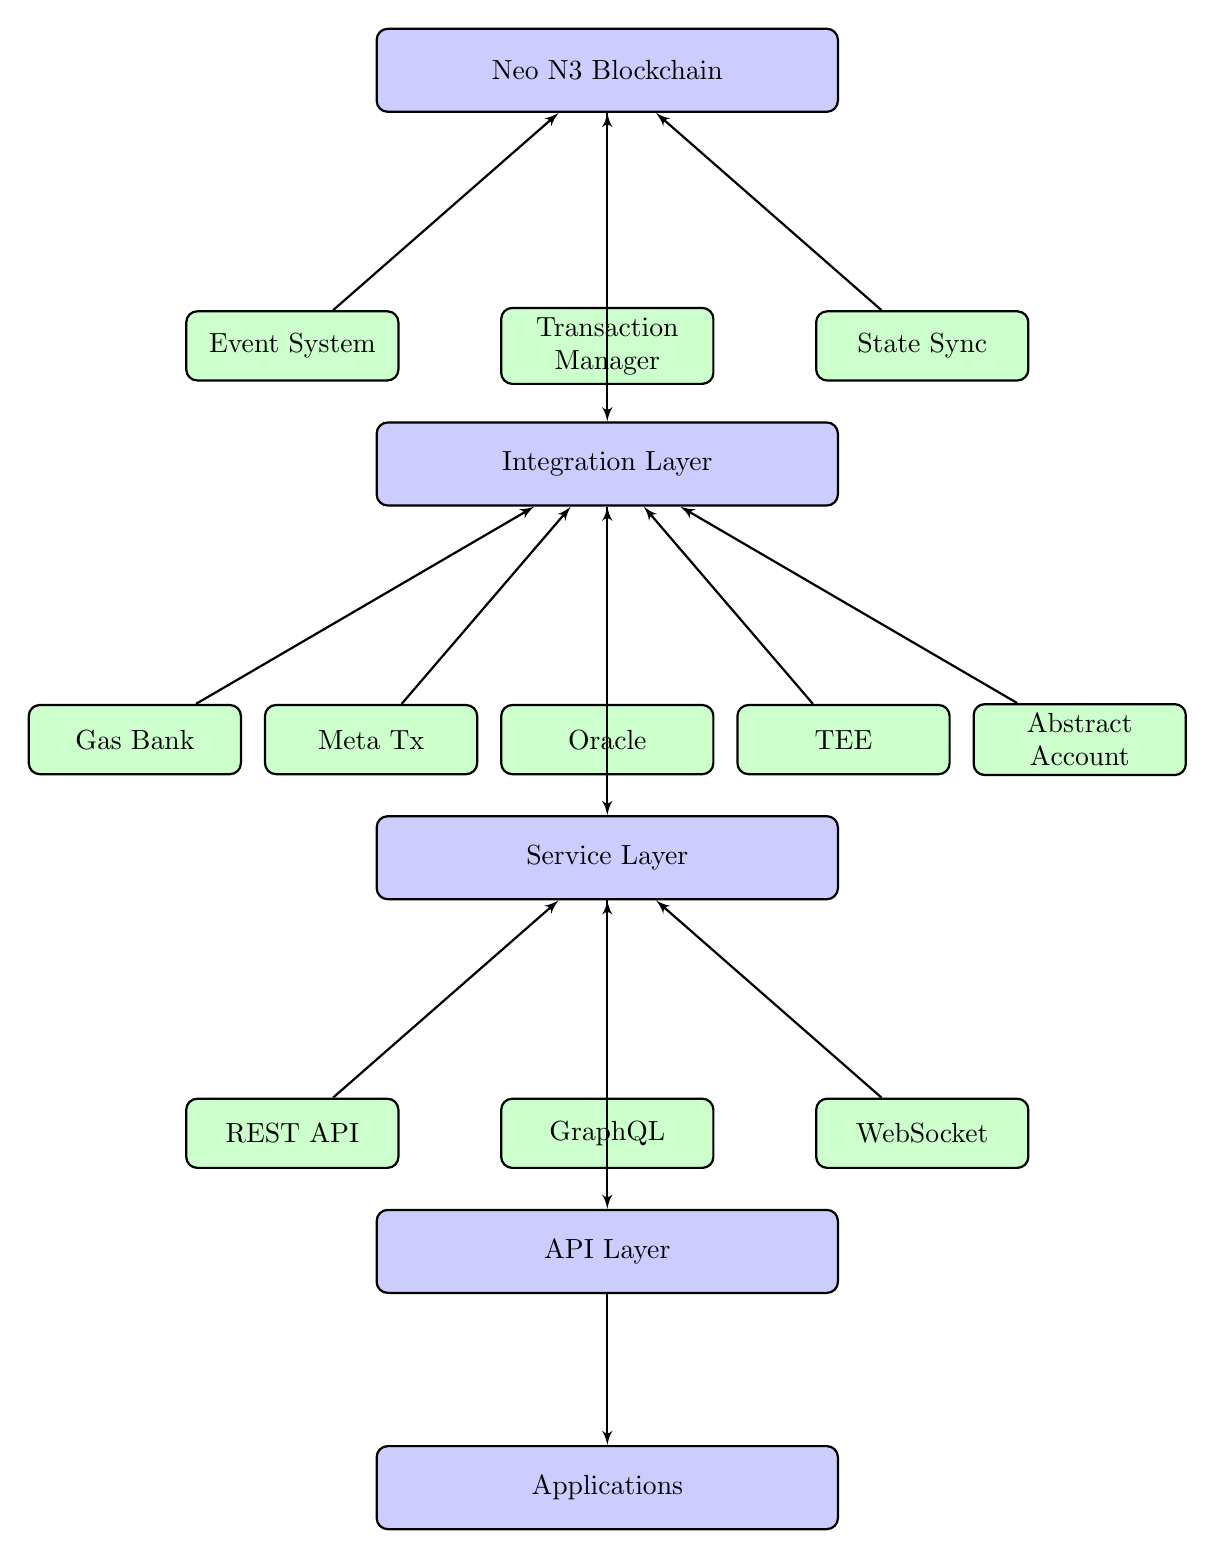
\begin{tikzpicture}[node distance=1.5cm, auto, thick]
    % Define styles
    \tikzstyle{layer} = [rectangle, draw, fill=blue!20, text width=16em, text centered, rounded corners, minimum height=3em]
    \tikzstyle{component} = [rectangle, draw, fill=green!20, text width=7em, text centered, rounded corners, minimum height=2.5em]
    \tikzstyle{line} = [draw, -latex']
    
    % Place nodes - layers
    \node [layer] (blockchain) {Neo N3 Blockchain};
    \node [layer, below of=blockchain, node distance=5cm] (integration) {Integration Layer};
    \node [layer, below of=integration, node distance=5cm] (service) {Service Layer};
    \node [layer, below of=service, node distance=5cm] (api) {API Layer};
    \node [layer, below of=api, node distance=3cm] (app) {Applications};
    
    % Place nodes - components in Integration Layer
    \node [component, above of=integration, node distance=1.5cm, xshift=-4cm] (event) {Event System};
    \node [component, above of=integration, node distance=1.5cm] (tx) {Transaction Manager};
    \node [component, above of=integration, node distance=1.5cm, xshift=4cm] (state) {State Sync};
    
    % Place nodes - components in Service Layer
    \node [component, above of=service, node distance=1.5cm, xshift=-6cm] (gas) {Gas Bank};
    \node [component, above of=service, node distance=1.5cm, xshift=-3cm] (meta) {Meta Tx};
    \node [component, above of=service, node distance=1.5cm] (oracle) {Oracle};
    \node [component, above of=service, node distance=1.5cm, xshift=3cm] (tee) {TEE};
    \node [component, above of=service, node distance=1.5cm, xshift=6cm] (account) {Abstract Account};
    
    % Place nodes - components in API Layer
    \node [component, above of=api, node distance=1.5cm, xshift=-4cm] (rest) {REST API};
    \node [component, above of=api, node distance=1.5cm] (graphql) {GraphQL};
    \node [component, above of=api, node distance=1.5cm, xshift=4cm] (websocket) {WebSocket};
    
    % Draw edges between layers
    \path [line] (blockchain) -- (integration);
    \path [line] (integration) -- (service);
    \path [line] (service) -- (api);
    \path [line] (api) -- (app);
    
    % Connect components to layers
    \path [line] (event) -- (blockchain);
    \path [line] (tx) -- (blockchain);
    \path [line] (state) -- (blockchain);
    
    \path [line] (gas) -- (integration);
    \path [line] (meta) -- (integration);
    \path [line] (oracle) -- (integration);
    \path [line] (tee) -- (integration);
    \path [line] (account) -- (integration);
    
    \path [line] (rest) -- (service);
    \path [line] (graphql) -- (service);
    \path [line] (websocket) -- (service);
    
\end{tikzpicture}
\caption{Neo Service Layer Architecture}
\label{fig:architecture}
\end{figure}


The architecture consists of several interconnected layers that work together to provide a comprehensive service infrastructure. At the foundation is the \textbf{Neo N3 Blockchain}, which provides the secure, deterministic execution environment for smart contracts and digital assets. Above this sits the \textbf{Integration Layer}, which connects the Neo blockchain with the Service Layer by handling event monitoring, transaction management, and state synchronization. The \textbf{Service Layer} forms the core of the Neo Service Layer, providing specialized services such as Gas Bank, Meta Transactions, Oracle Services, and Trusted Execution Environments. The \textbf{API Layer} exposes service functionalities through standardized interfaces, including RESTful APIs, GraphQL endpoints, and WebSocket connections, making the services accessible to developers. At the top level are the \textbf{Applications}, user-facing software that leverages the Neo Service Layer to provide enhanced functionality and user experiences.

This layered approach ensures clear separation of concerns while enabling seamless integration between components. Each layer implements specific security controls, creating a defense-in-depth model that protects against threats at multiple levels while maintaining the performance characteristics necessary for commercial applications.

\subsection{Core Services}
\label{subsec:nsl-core-services}

The Neo Service Layer provides several core services that enhance the capabilities of Neo Smart Contracts and improve the user experience. These services address common challenges in blockchain application development and enable new use cases that would be difficult or impossible to implement using on-chain logic alone.

\subsubsection{Gas Bank}
\label{subsubsec:gas-bank}

The Gas Bank service provides a solution to one of the most significant barriers to blockchain adoption: the requirement for users to hold native tokens (GAS) to pay for transaction fees. This requirement creates friction for new users and limits the adoption of decentralized applications.

\begin{figure}[h]
\centering
\begin{tcolorbox}[
    enhanced,
    colback=blue!5!white,
    colframe=blue!75!black,
    arc=5mm,
    boxrule=1.5pt,
    title=Gas Bank Architecture,
    fonttitle=\bfseries,
    coltitle=white,
    attach boxed title to top left={yshift=-2mm, xshift=5mm},
    boxed title style={colback=blue!75!black, rounded corners},
    shadow={2mm}{-2mm}{0mm}{black!50},
    drop fuzzy shadow
]
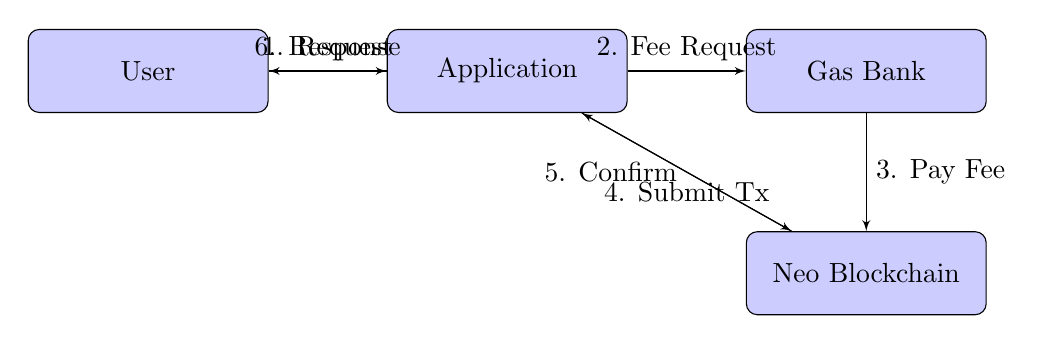
\begin{tikzpicture}[node distance=1.5cm, auto]
    % Define styles
    \tikzstyle{block} = [rectangle, draw, fill=blue!20, text width=8em, text centered, rounded corners, minimum height=3em]
    \tikzstyle{line} = [draw, -latex']
    \tikzstyle{cloud} = [draw, ellipse, fill=red!20, node distance=3cm, minimum height=2em]
    
    % Place nodes
    \node [block] (user) {User};
    \node [block, right=of user] (app) {Application};
    \node [block, right=of app] (gasbank) {Gas Bank};
    \node [block, below=of gasbank] (blockchain) {Neo Blockchain};
    
    % Draw edges
    \path [line] (user) -- node {1. Request} (app);
    \path [line] (app) -- node {2. Fee Request} (gasbank);
    \path [line] (gasbank) -- node {3. Pay Fee} (blockchain);
    \path [line] (app) -- node [below] {4. Submit Tx} (blockchain);
    \path [line] (blockchain) -- node [left] {5. Confirm} (app);
    \path [line] (app) -- node [above] {6. Response} (user);
\end{tikzpicture}
\end{tcolorbox}
\caption{Gas Bank Architecture and Transaction Flow}
\label{fig:gas-bank-architecture}
\end{figure}


The Gas Bank allows application developers to create accounts that can pay for transaction fees on behalf of their users, enabling a seamless user experience similar to traditional web applications. Users can interact with decentralized applications without needing to acquire GAS tokens first, removing a significant barrier to entry.

\begin{definition}[Gas Bank Account]
A Gas Bank Account is a managed account that holds GAS tokens and can be used to pay for transaction fees on behalf of users. Each account has the following properties:
\begin{itemize}
    \item Address: The unique identifier of the account
    \item Balance: The amount of GAS tokens available for fee payment
    \item Fee Model: The fee calculation model (fixed, percentage, dynamic, or free)
    \item Credit Limit: The maximum amount of credit that can be extended to the account
    \item Used Credit: The amount of credit currently used
    \item Status: The current status of the account (active, suspended, etc.)
\end{itemize}
\end{definition}

The Gas Bank supports multiple fee models to accommodate different application requirements. The \textbf{Fixed Fee} model applies a constant fee regardless of the transaction size or complexity, providing predictability for users and developers. The \textbf{Percentage Fee} model calculates fees as a percentage of the transaction amount, which is particularly useful for value transfer operations where the fee scales with the transaction value. For applications requiring more adaptive pricing, the \textbf{Dynamic Fee} model varies based on network conditions and transaction complexity, optimizing for both cost and confirmation time. Some applications may choose the \textbf{Free} model where no fee is charged to the user, with all costs absorbed by the application to provide a seamless user experience similar to traditional web applications.

The Gas Bank service also provides credit facilities, allowing applications to continue operating even when their Gas Bank account balance is temporarily depleted. This feature ensures uninterrupted service for users while giving application developers time to replenish their accounts.

\begin{figure}[h]
\centering
\begin{tcolorbox}[
    enhanced,
    colback=blue!5!white,
    colframe=blue!75!black,
    arc=5mm,
    boxrule=1.5pt,
    title=Gas Bank Architecture,
    fonttitle=\bfseries,
    coltitle=white,
    attach boxed title to top left={yshift=-2mm, xshift=5mm},
    boxed title style={colback=blue!75!black, rounded corners},
    shadow={2mm}{-2mm}{0mm}{black!50},
    drop fuzzy shadow
]
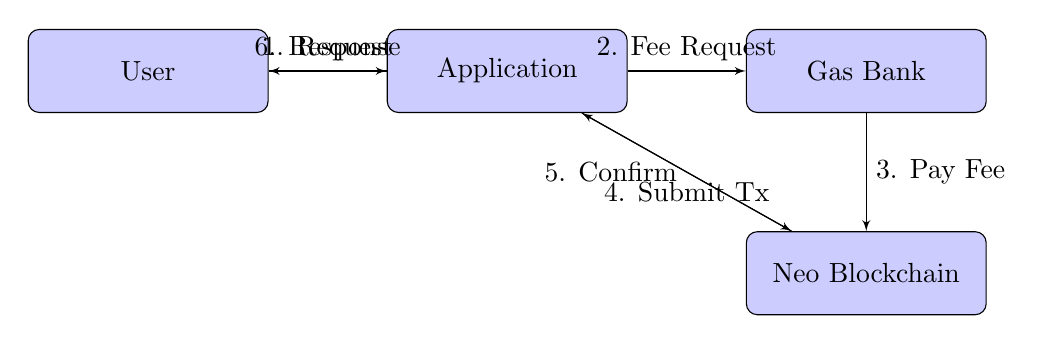
\begin{tikzpicture}[node distance=1.5cm, auto]
    % Define styles
    \tikzstyle{block} = [rectangle, draw, fill=blue!20, text width=8em, text centered, rounded corners, minimum height=3em]
    \tikzstyle{line} = [draw, -latex']
    \tikzstyle{cloud} = [draw, ellipse, fill=red!20, node distance=3cm, minimum height=2em]
    
    % Place nodes
    \node [block] (user) {User};
    \node [block, right=of user] (app) {Application};
    \node [block, right=of app] (gasbank) {Gas Bank};
    \node [block, below=of gasbank] (blockchain) {Neo Blockchain};
    
    % Draw edges
    \path [line] (user) -- node {1. Request} (app);
    \path [line] (app) -- node {2. Fee Request} (gasbank);
    \path [line] (gasbank) -- node {3. Pay Fee} (blockchain);
    \path [line] (app) -- node [below] {4. Submit Tx} (blockchain);
    \path [line] (blockchain) -- node [left] {5. Confirm} (app);
    \path [line] (app) -- node [above] {6. Response} (user);
\end{tikzpicture}
\end{tcolorbox}
\caption{Gas Bank Architecture and Transaction Flow}
\label{fig:gas-bank-architecture}
\end{figure}


\paragraph{Deposit and Withdrawal Operations}
The Gas Bank implements a comprehensive system for managing deposits and withdrawals. \textbf{User Deposits} allow individuals to deposit GAS tokens into the Gas Bank through direct blockchain transactions or application interfaces, with each deposit verified on-chain and credited to the appropriate account. For developers, \textbf{Application Deposits} provide a way to fund their Gas Bank accounts through direct deposits or automated funding mechanisms, ensuring sufficient balance for covering user transaction fees. The \textbf{Withdrawal Process} enables account owners to withdraw their GAS tokens through a secure process that includes verification of ownership, balance checks, and transaction confirmation to prevent unauthorized access. To maintain operational continuity, \textbf{Automated Refills} can be configured by applications to trigger deposits from designated funding sources when account balances fall below specified thresholds, preventing service interruptions due to insufficient funds.

A formal specification of the Gas Bank operations protocol is provided in Section \ref{subsec:gas-bank-protocol}.

\subsection{Gas Bank Protocol}
\label{subsec:gas-bank-protocol}

The Gas Bank Protocol defines how users and applications can deposit, withdraw, and use GAS tokens for transaction fee payment.

\begin{tcolorbox}[
    enhanced,
    colback=blue!5!white,
    colframe=blue!75!black,
    arc=5mm,
    boxrule=1.5pt,
    title=Gas Bank Deposit Protocol,
    fonttitle=\bfseries,
    coltitle=white,
    attach boxed title to top left={yshift=-2mm, xshift=5mm},
    boxed title style={colback=blue!75!black, rounded corners},
    shadow={2mm}{-2mm}{0mm}{black!50},
    drop fuzzy shadow
]
\begin{protocol}{Gas Bank Deposit}
\label{prot:gas-bank-deposit}
\begin{algorithmic}[1]
\Require User $U$, Amount $A$, Gas Bank $G$, Neo Blockchain $B$
\Ensure GAS tokens are securely deposited into the Gas Bank

\State \textbf{Authentication:}
\State $\text{authenticated} \gets \text{AuthenticateUser}(U)$
\If{$\neg \text{authenticated}$}
    \State \textbf{reject} with "Authentication failed"
\EndIf

\State \textbf{Account Verification:}
\State $\text{account} \gets G.\text{getAccount}(U.\text{address})$
\If{$\text{account} = \text{null}$}
    \State $\text{account} \gets G.\text{createAccount}(U.\text{address})$
\EndIf

\State \textbf{Transaction Creation:}
\State $\text{tx} \gets \text{CreateTransaction}(U.\text{address}, G.\text{address}, A, \text{"GAS"})$
\State $\text{tx}.\text{setRemark}(\text{"Gas Bank Deposit"})$

\State \textbf{Transaction Signing:}
\State $\text{signature} \gets U.\text{sign}(\text{tx})$
\State $\text{tx}.\text{addWitness}(\text{signature})$

\State \textbf{Transaction Submission:}
\State $\text{txid} \gets B.\text{submitTransaction}(\text{tx})$

\State \textbf{Transaction Monitoring:}
\State $\text{status} \gets \text{MonitorTransaction}(\text{txid})$
\If{$\text{status} \neq \text{"confirmed"}$}
    \State \textbf{reject} with "Transaction failed: " + $\text{status}$
\EndIf

\State \textbf{Balance Update:}
\State $\text{account}.\text{balance} \gets \text{account}.\text{balance} + A$
\State $G.\text{updateAccount}(\text{account})$

\State \textbf{Event Emission:}
\State $G.\text{emitEvent}(\text{"Deposit"}, \{U.\text{address}, A, \text{txid}\})$

\State \Return $\{\text{status}: \text{"success"}, \text{txid}: \text{txid}, \text{balance}: \text{account}.\text{balance}\}$
\end{algorithmic}
\end{protocol}
\end{tcolorbox}

\begin{tcolorbox}[
    enhanced,
    colback=blue!5!white,
    colframe=blue!75!black,
    arc=5mm,
    boxrule=1.5pt,
    title=Gas Bank Withdrawal Protocol,
    fonttitle=\bfseries,
    coltitle=white,
    attach boxed title to top left={yshift=-2mm, xshift=5mm},
    boxed title style={colback=blue!75!black, rounded corners},
    shadow={2mm}{-2mm}{0mm}{black!50},
    drop fuzzy shadow
]
\begin{protocol}{Gas Bank Withdrawal}
\label{prot:gas-bank-withdrawal}
\begin{algorithmic}[1]
\Require User $U$, Amount $A$, Gas Bank $G$, Neo Blockchain $B$
\Ensure GAS tokens are securely withdrawn from the Gas Bank

\State \textbf{Authentication:}
\State $\text{authenticated} \gets \text{AuthenticateUser}(U)$
\If{$\neg \text{authenticated}$}
    \State \textbf{reject} with "Authentication failed"
\EndIf

\State \textbf{Account Verification:}
\State $\text{account} \gets G.\text{getAccount}(U.\text{address})$
\If{$\text{account} = \text{null}$}
    \State \textbf{reject} with "Account not found"
\EndIf

\State \textbf{Balance Check:}
\If{$\text{account}.\text{balance} < A$}
    \State \textbf{reject} with "Insufficient balance"
\EndIf

\State \textbf{Transaction Creation:}
\State $\text{tx} \gets \text{CreateTransaction}(G.\text{address}, U.\text{address}, A, \text{"GAS"})$
\State $\text{tx}.\text{setRemark}(\text{"Gas Bank Withdrawal"})$

\State \textbf{Transaction Signing:}
\State $\text{signature} \gets G.\text{sign}(\text{tx})$
\State $\text{tx}.\text{addWitness}(\text{signature})$

\State \textbf{Transaction Submission:}
\State $\text{txid} \gets B.\text{submitTransaction}(\text{tx})$

\State \textbf{Transaction Monitoring:}
\State $\text{status} \gets \text{MonitorTransaction}(\text{txid})$
\If{$\text{status} \neq \text{"confirmed"}$}
    \State \textbf{reject} with "Transaction failed: " + $\text{status}$
\EndIf

\State \textbf{Balance Update:}
\State $\text{account}.\text{balance} \gets \text{account}.\text{balance} - A$
\State $G.\text{updateAccount}(\text{account})$

\State \textbf{Event Emission:}
\State $G.\text{emitEvent}(\text{"Withdrawal"}, \{U.\text{address}, A, \text{txid}\})$

\State \Return $\{\text{status}: \text{"success"}, \text{txid}: \text{txid}, \text{balance}: \text{account}.\text{balance}\}$
\end{algorithmic}
\end{protocol}
\end{tcolorbox}

\begin{tcolorbox}[
    enhanced,
    colback=blue!5!white,
    colframe=blue!75!black,
    arc=5mm,
    boxrule=1.5pt,
    title=Gas Bank Fee Payment Protocol,
    fonttitle=\bfseries,
    coltitle=white,
    attach boxed title to top left={yshift=-2mm, xshift=5mm},
    boxed title style={colback=blue!75!black, rounded corners},
    shadow={2mm}{-2mm}{0mm}{black!50},
    drop fuzzy shadow
]
\begin{protocol}{Gas Bank Fee Payment}
\label{prot:gas-bank-fee-payment}
\begin{algorithmic}[1]
\Require User $U$, Application $A$, Transaction $T$, Gas Bank $G$, Neo Blockchain $B$
\Ensure Transaction fees are paid by the Gas Bank on behalf of the user

\State \textbf{Application Verification:}
\State $\text{app\_account} \gets G.\text{getApplicationAccount}(A.\text{id})$
\If{$\text{app\_account} = \text{null}$}
    \State \textbf{reject} with "Application not registered"
\EndIf

\State \textbf{Fee Calculation:}
\State $\text{fee} \gets \text{CalculateFee}(T, \text{app\_account}.\text{fee\_model})$

\State \textbf{Balance Check:}
\If{$\text{app\_account}.\text{balance} < \text{fee}$}
    \If{$\text{app\_account}.\text{credit\_enabled}$}
        \If{$\text{app\_account}.\text{used\_credit} + \text{fee} > \text{app\_account}.\text{credit\_limit}$}
            \State \textbf{reject} with "Credit limit exceeded"
        \EndIf
        \State $\text{app\_account}.\text{used\_credit} \gets \text{app\_account}.\text{used\_credit} + \text{fee}$
    \Else
        \State \textbf{reject} with "Insufficient balance"
    \EndIf
\Else
    \State $\text{app\_account}.\text{balance} \gets \text{app\_account}.\text{balance} - \text{fee}$
\EndIf

\State \textbf{Transaction Modification:}
\State $T.\text{setSystemFee}(\text{fee})$
\State $T.\text{setNetworkFee}(0)$
\State $T.\text{addAttribute}(\text{"GasBank"}, G.\text{address})$

\State \textbf{Transaction Signing:}
\State $\text{signature} \gets G.\text{sign}(T)$
\State $T.\text{addWitness}(\text{signature})$

\State \textbf{Transaction Submission:}
\State $\text{txid} \gets B.\text{submitTransaction}(T)$

\State \textbf{Account Update:}
\State $G.\text{updateApplicationAccount}(\text{app\_account})$

\State \textbf{Usage Logging:}
\State $G.\text{logUsage}(A.\text{id}, U.\text{address}, \text{fee}, \text{txid})$

\State \Return $\{\text{status}: \text{"success"}, \text{txid}: \text{txid}, \text{fee}: \text{fee}\}$
\end{algorithmic}
\end{protocol}
\end{tcolorbox}


\paragraph{Fee Calculation and Payment}
When a user interacts with an application that uses the Gas Bank:

\begin{enumerate}
    \item The application requests fee payment from the Gas Bank service.
    \item The Gas Bank calculates the required fee based on the configured fee model.
    \item The Gas Bank verifies that the application's account has sufficient balance.
    \item If sufficient balance exists, the Gas Bank authorizes the transaction and reserves the fee amount.
    \item Once the transaction is confirmed on the blockchain, the Gas Bank deducts the actual fee from the reserved amount and releases any excess.
    \item The application receives confirmation of the fee payment and can update its records accordingly.
\end{enumerate}

\paragraph{Multi-Chain Support}
The Gas Bank service supports multiple blockchain networks to provide a unified fee management solution across different ecosystems. It offers \textbf{Neo N3} native support with comprehensive GAS token fee management tailored to the Neo blockchain's specific requirements. For projects operating on Ethereum or EVM-compatible chains, the service provides \textbf{Ethereum} support with ETH fee management capabilities, allowing developers to use the same service interface across different blockchain environments. The system also enables \textbf{Cross-Chain Operations} with the ability to manage fees across different blockchain networks through integrated bridges and conversion mechanisms, creating a seamless experience for applications that operate in multi-chain environments.

This multi-chain capability enables applications to provide a consistent user experience across different blockchain ecosystems while centralizing fee management in a single service.

\subsubsection{Meta Transaction Service}
\label{subsubsec:meta-tx}

Meta transactions enable users to interact with smart contracts without directly paying for transaction fees, further reducing the barriers to blockchain adoption. The Meta Transaction Service acts as a relay that receives signed transaction requests from users, verifies their validity, and submits them to the blockchain on behalf of the users.

% This file should only be \input{} in a document that loads the tikz package
% Do not compile this file directly with pdflatex

\begin{figure}[ht]
\centering
\begin{tikzpicture}[font=\scriptsize, node distance=3cm]
    % Define nodes
    \node[cloud] (user) at (0,0) {User};
    \node[box] (relay) at (4,0) {Meta-TX Relay};
    \node[box] (chain) at (8,0) {Blockchain};
    
    % Define connections
    \draw[connector] (user) -- node[above-arrow-text] {1. Sign transaction} (relay);
    \draw[connector] (relay) to[bend left=20] node[above-arrow-text] {2. Submit transaction} (chain);
    \draw[connector] (chain) to[bend left=20] node[below-arrow-text] {3. Confirm transaction} (relay);
    \draw[connector] (relay) -- node[below-arrow-text] {4. Notify user} (user);
\end{tikzpicture}
\caption{Meta-Transaction Flow}
\label{fig:meta-tx-flow}
\end{figure}


\begin{definition}[Meta Transaction]
A Meta Transaction is a transaction request that is signed by a user but submitted to the blockchain by a relayer. The relayer pays for the transaction fees, while the transaction itself is executed as if it were submitted by the original user.
\end{definition}

The Meta Transaction Service supports multiple blockchain types and signature curves, enabling interoperability between Neo N3 and other blockchain ecosystems. It provides full support for \textbf{Neo N3 with secp256r1} curve for standard Neo N3 transactions and signatures, ensuring compatibility with the Neo ecosystem. Additionally, it supports \textbf{Ethereum with secp256k1} curve for Ethereum-compatible transactions and signatures, including EIP-712 typed data signing, which enables secure structured data signing for enhanced security and user experience.

This cross-chain compatibility is particularly valuable for applications that operate across multiple blockchain ecosystems, as it allows users to interact with contracts on different chains using a single signature mechanism.

The Meta Transaction Service integrates with the Gas Bank to pay for transaction fees, creating a comprehensive solution for fee abstraction. Application developers can configure the service to use specific Gas Bank accounts for different contracts or transaction types, enabling fine-grained control over fee allocation.

\begin{figure}[ht]
    \centering
    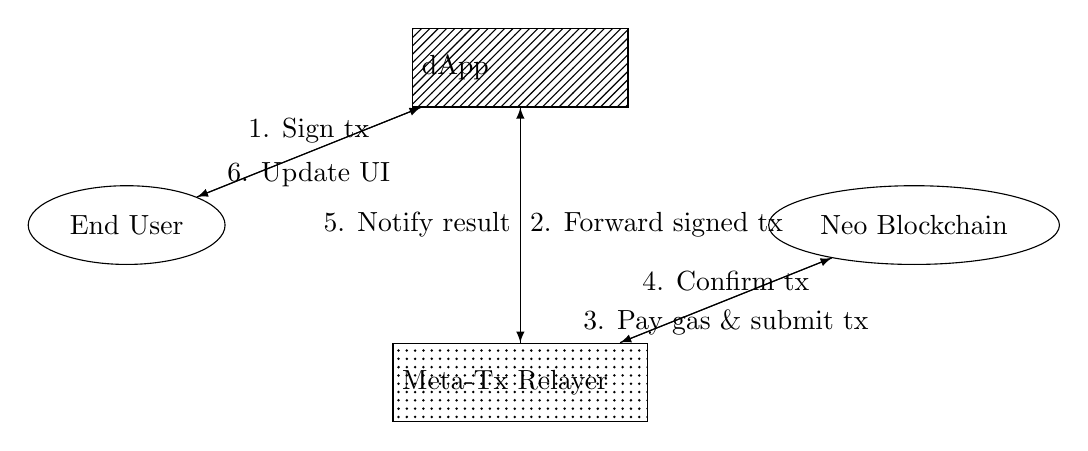
\begin{tikzpicture}
        % Define nodes
        \node[cloud, minimum width=2.5cm] (user) at (-5,2) {End User};
        \node[box=north east lines, text width=2.5cm] (dapp) at (0,4) {dApp};
        \node[box=dots, text width=3cm] (relay) at (0,0) {Meta-Tx Relayer};
        \node[cloud, minimum width=3cm] (neo) at (5,2) {Neo Blockchain};
        
        % Define connections
        \path [line] (user) -- node[above] {1. Sign tx} (dapp);
        \path [line] (dapp) -- node[right] {2. Forward signed tx} (relay);
        \path [line] (relay) -- node[below] {3. Pay gas \& submit tx} (neo);
        \path [line] (neo) -- node[above] {4. Confirm tx} (relay);
        \path [line] (relay) -- node[left] {5. Notify result} (dapp);
        \path [line] (dapp) -- node[below] {6. Update UI} (user);
    \end{tikzpicture}
    \caption{Meta-Transaction Flow}
    \label{fig:meta-transaction}
\end{figure}


\paragraph{Meta Transaction Workflow}
The complete workflow for processing a meta transaction involves several steps:

\begin{enumerate}
    \item \textbf{Transaction Creation}: The user creates a transaction request containing the target contract, method, parameters, and any other required information.
    
    \item \textbf{Signature Generation}: The user signs the transaction request using their private key. For Neo N3, this uses the secp256r1 curve, while for Ethereum-compatible transactions, secp256k1 is used with EIP-712 typed data signing.
    
    \item \textbf{Relay Submission}: The signed transaction request is submitted to the Meta Transaction Service through its API.
    
    \item \textbf{Signature Verification}: The service verifies the signature to ensure the request was genuinely signed by the claimed user.
    
    \item \textbf{Fee Estimation}: The service estimates the required transaction fee based on the current network conditions and transaction complexity.
    
    \item \textbf{Gas Bank Integration}: The service requests fee payment from the Gas Bank service, specifying the application account that should cover the cost.
    
    \item \textbf{Transaction Submission}: Upon successful fee authorization, the service constructs and submits the transaction to the blockchain network.
    
    \item \textbf{Confirmation Monitoring}: The service monitors the transaction until it is confirmed on the blockchain.
    
    \item \textbf{Result Notification}: The service notifies the application of the transaction result, including success status, transaction hash, and any return values.
\end{enumerate}

A formal specification of the Meta Transaction protocol is provided in Section \ref{subsec:meta-tx-protocol}.

\subsection{Meta Transaction Protocol}
\label{subsec:meta-tx-protocol}

The Meta Transaction Protocol defines how users can interact with smart contracts without directly paying for transaction fees.

\begin{tcolorbox}[
    enhanced,
    colback=blue!5!white,
    colframe=blue!75!black,
    arc=5mm,
    boxrule=1.5pt,
    title=Meta Tx Protocol,
    fonttitle=\bfseries,
    coltitle=white,
    attach boxed title to top left={yshift=-2mm, xshift=5mm},
    boxed title style={colback=blue!75!black, rounded corners},
    shadow={2mm}{-2mm}{0mm}{black!50},
    drop fuzzy shadow
]
\begin{tcolorbox}[
    enhanced,
    colback=blue!5!white,
    colframe=blue!75!black,
    arc=5mm,
    boxrule=1.5pt,
    title=Protocol,
    fonttitle=\bfseries,
    coltitle=white,
    attach boxed title to top left={yshift=-2mm, xshift=5mm},
    boxed title style={colback=blue!75!black, rounded corners},
    shadow={2mm}{-2mm}{0mm}{black!50},
    drop fuzzy shadow
]
\begin{protocol}{Meta Transaction Processing}
\label{prot:meta-tx-processing}
\begin{algorithmic}[1]
\Require User $U$, Transaction request $R$, Meta Transaction Service $M$, Gas Bank Service $G$, Blockchain $B$
\Ensure Transaction is executed on behalf of the user without requiring user to pay fees

\State \textbf{Transaction Creation:}
\State $\text{txData} \gets \{\text{to}: R.\text{to}, \text{data}: R.\text{data}, \text{value}: R.\text{value}, \text{nonce}: U.\text{nonce}, \text{chainId}: B.\text{chainId}\}$

\State \textbf{Signature Generation:}
\State $\text{message} \gets \text{FormatMessage}(\text{txData})$
\State $\text{signature} \gets U.\text{sign}(\text{message})$

\State \textbf{Meta Transaction Request:}
\State $\text{metaTx} \gets \{\text{txData}: \text{txData}, \text{signature}: \text{signature}, \text{from}: U.\text{address}\}$
\State $M.\text{submitTransaction}(\text{metaTx})$

\State \textbf{Signature Verification:}
\State $\text{recoveredAddress} \gets \text{RecoverSigner}(\text{message}, \text{signature})$
\If{$\text{recoveredAddress} \neq U.\text{address}$}
    \State \Return $\{\text{error}: \text{"Invalid signature"}\}$
\EndIf

\State \textbf{Nonce Verification:}
\State $\text{expectedNonce} \gets M.\text{getNonce}(U.\text{address})$
\If{$\text{txData}.\text{nonce} \neq \text{expectedNonce}$}
    \State \Return $\{\text{error}: \text{"Invalid nonce"}\}$
\EndIf

\State \textbf{Fee Estimation:}
\State $\text{gasLimit} \gets B.\text{estimateGas}(\text{txData})$
\State $\text{gasPrice} \gets B.\text{getGasPrice}()$
\State $\text{fee} \gets \text{gasLimit} \times \text{gasPrice}$

\State \textbf{Gas Bank Integration:}
\State $\text{app} \gets M.\text{getApplicationForContract}(\text{txData}.\text{to})$
\State $\text{account} \gets G.\text{getAccountForApplication}(\text{app}.\text{id})$
\State $\text{feeApproval} \gets G.\text{requestFeePayment}(\text{app}, \text{account}, \text{fee})$
\If{$\neg \text{feeApproval}.\text{approved}$}
    \State \Return $\{\text{error}: \text{"Fee payment not approved"}, \text{reason}: \text{feeApproval}.\text{reason}\}$
\EndIf

\State \textbf{Transaction Construction:}
\State $\text{rawTx} \gets B.\text{createTransaction}(\{\text{from}: M.\text{relayerAddress}, \text{to}: \text{txData}.\text{to}, \text{data}: \text{EncodeWithSender}(\text{txData}.\text{data}, U.\text{address}), \text{value}: \text{txData}.\text{value}, \text{gasLimit}: \text{gasLimit}, \text{gasPrice}: \text{gasPrice}\})$
\State $\text{signedTx} \gets M.\text{signTransaction}(\text{rawTx})$

\State \textbf{Transaction Submission:}
\State $\text{txHash} \gets B.\text{submitTransaction}(\text{signedTx})$

\State \textbf{Transaction Monitoring:}
\State $\text{confirmed} \gets \text{false}$
\While{$\neg \text{confirmed}$}
    \State $\text{receipt} \gets B.\text{getTransactionReceipt}(\text{txHash})$
    \If{$\text{receipt} \neq \text{null}$}
        \State $\text{confirmed} \gets \text{true}$
        \If{$\text{receipt}.\text{status} = \text{"success"}$}
            \State $M.\text{incrementNonce}(U.\text{address})$
            \State $G.\text{confirmFeePayment}(\text{app}, \text{account}, \text{receipt}.\text{gasUsed} \times \text{receipt}.\text{gasPrice})$
        \Else
            \State $G.\text{cancelFeePayment}(\text{app}, \text{account}, \text{feeApproval}.\text{id})$
        \EndIf
    \EndIf
    \If{$\neg \text{confirmed}$}
        \State $\text{Sleep}(1\text{ second})$
    \EndIf
\EndWhile

\State \textbf{Result Notification:}
\State $M.\text{notifyResult}(U.\text{address}, \text{txHash}, \text{receipt})$

\State \Return $\{\text{success}: \text{receipt}.\text{status} = \text{"success"}, \text{txHash}: \text{txHash}, \text{receipt}: \text{receipt}\}$
\end{algorithmic}
\end{protocol}
\end{tcolorbox}


\begin{tcolorbox}[
    enhanced,
    colback=blue!5!white,
    colframe=blue!75!black,
    arc=5mm,
    boxrule=1.5pt,
    title=Meta Tx Protocol,
    fonttitle=\bfseries,
    coltitle=white,
    attach boxed title to top left={yshift=-2mm, xshift=5mm},
    boxed title style={colback=blue!75!black, rounded corners},
    shadow={2mm}{-2mm}{0mm}{black!50},
    drop fuzzy shadow
]
\begin{tcolorbox}[
    enhanced,
    colback=blue!5!white,
    colframe=blue!75!black,
    arc=5mm,
    boxrule=1.5pt,
    title=Protocol,
    fonttitle=\bfseries,
    coltitle=white,
    attach boxed title to top left={yshift=-2mm, xshift=5mm},
    boxed title style={colback=blue!75!black, rounded corners},
    shadow={2mm}{-2mm}{0mm}{black!50},
    drop fuzzy shadow
]
\begin{protocol}{EIP-712 Signature Verification}
\label{prot:eip712-verification}
\begin{algorithmic}[1]
\Require Transaction data $D$, Signature $S$, Claimed signer $A$, Domain separator $\text{DS}$, Type hash $\text{TH}$
\Ensure Signature is valid and matches the claimed signer

\State \textbf{Type Hash Calculation:}
\State $\text{typeHash} \gets \text{TH}$

\State \textbf{Value Hash Calculation:}
\State $\text{encodedData} \gets \text{EncodeData}(D)$
\State $\text{valueHash} \gets \text{keccak256}(\text{encodedData})$

\State \textbf{Message Hash Calculation:}
\State $\text{message} \gets \text{"\textbackslash x19\textbackslash x01"} \parallel \text{DS} \parallel \text{keccak256}(\text{typeHash} \parallel \text{valueHash})$
\State $\text{messageHash} \gets \text{keccak256}(\text{message})$

\State \textbf{Signature Components:}
\State $r \gets S[0:32]$
\State $s \gets S[32:64]$
\State $v \gets S[64]$

\State \textbf{Address Recovery:}
\State $\text{recoveredAddress} \gets \text{ecrecover}(\text{messageHash}, v, r, s)$

\If{$\text{recoveredAddress} = A$}
    \State \Return $\text{true}$
\Else
    \State \Return $\text{false}$
\EndIf
\end{algorithmic}
\end{protocol}
\end{tcolorbox}



\paragraph{Signature Verification Protocol}
The Meta Transaction Service implements a robust signature verification protocol that supports multiple signature schemes. For Neo N3 transactions, the service performs \textbf{Neo N3 Verification} by verifying secp256r1 signatures against the transaction hash, ensuring the signature matches the claimed sender's public key and maintaining the security model of the Neo blockchain. When handling Ethereum-compatible transactions, the service implements \textbf{EIP-712 Verification} using the EIP-712 standard for typed data signing, which provides enhanced security by having users sign structured data rather than raw transaction bytes, making the signing process more transparent and secure for users. For applications that operate across multiple blockchain networks, the service supports \textbf{Cross-Chain Verification} by verifying signatures using the appropriate scheme for each chain, enabling seamless cross-chain interactions while maintaining the security guarantees of each underlying blockchain.

\paragraph{Replay Protection}
To prevent replay attacks, where a valid transaction is maliciously resubmitted, the Meta Transaction Service implements several comprehensive protection mechanisms. The service employs \textbf{Nonce Tracking} where each user account has an associated nonce that must be included in the transaction and incremented with each submission, ensuring transactions can only be processed once in the correct order. For time-sensitive operations, \textbf{Timestamp Validation} is implemented, where transactions include a timestamp and are rejected if they are too old or too far in the future, creating a time window for valid submissions. To prevent cross-chain replay attacks, \textbf{Chain ID Inclusion} ensures that transactions include a chain identifier, preventing the same transaction from being replayed on different blockchain networks. Additionally, the service maintains a \textbf{Transaction Hash Registry} of processed transaction hashes to provide an extra layer of protection against duplicate submissions, even in edge cases where other protection mechanisms might not catch a replay attempt.

\subsubsection{Oracle Service}
\label{subsubsec:oracle}

Blockchain smart contracts operate in a deterministic environment isolated from external data sources. This isolation ensures security and predictability but limits the types of applications that can be built using smart contracts alone. The Oracle Service bridges this gap by providing a secure and reliable way for smart contracts to access external data.

\begin{figure}[htbp]
\centering
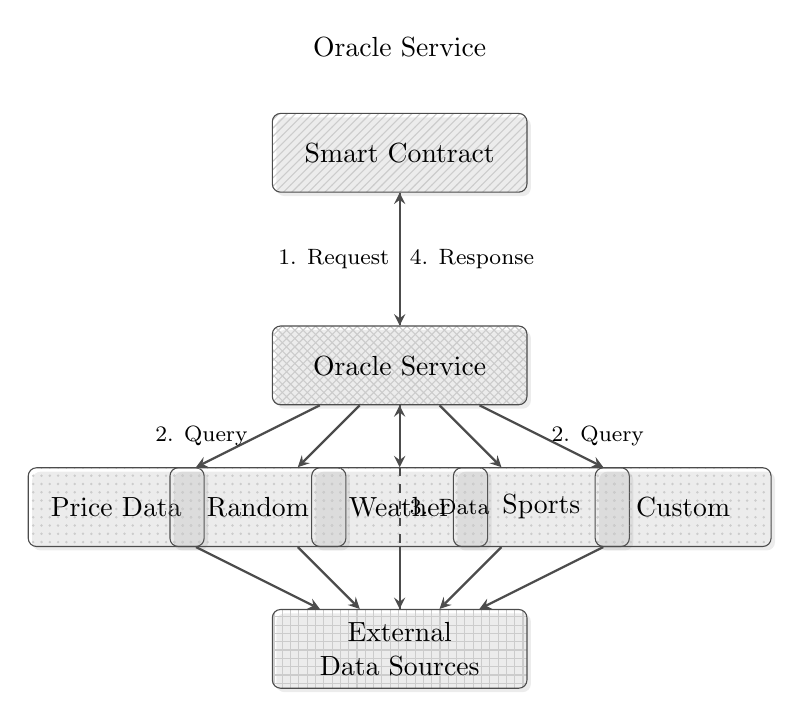
\begin{tikzpicture}[
    scale=0.9,
    box/.style={rectangle, draw=black!70, rounded corners=3pt, 
               fill=white, text width=3cm, align=center, minimum height=1cm,
               pattern=#1, pattern color=black!20,
               drop shadow={opacity=0.15, shadow xshift=0.5mm, shadow yshift=-0.5mm}},
    arrow/.style={->, >=stealth, thick, draw=black!70},
    dashed_arrow/.style={->, >=stealth, thick, dashed, draw=black!70}
]

% Oracle Components
\node[box=north east lines] (contract) at (0,3) {Smart Contract};
\node[box=crosshatch] (oracle) at (0,0) {Oracle Service};

% Data Sources
\node[box=dots, text width=2cm] (price) at (-4,-2) {Price Data};
\node[box=dots, text width=2cm] (random) at (-2,-2) {Random};
\node[box=dots, text width=2cm] (weather) at (0,-2) {Weather};
\node[box=dots, text width=2cm] (sports) at (2,-2) {Sports};
\node[box=dots, text width=2cm] (custom) at (4,-2) {Custom};

% External Systems
\node[box=grid] (external) at (0,-4) {External Data Sources};

% Arrows
\draw[arrow] (contract) -- node[left, font=\footnotesize] {1. Request} (oracle);
\draw[dashed_arrow] (oracle) -- node[right, font=\footnotesize] {4. Response} (contract);

\draw[arrow] (oracle) -- node[left, font=\footnotesize] {2. Query} (price);
\draw[arrow] (oracle) -- (random);
\draw[arrow] (oracle) -- (weather);
\draw[arrow] (oracle) -- (sports);
\draw[arrow] (oracle) -- node[right, font=\footnotesize] {2. Query} (custom);

\draw[arrow] (price) -- (external);
\draw[arrow] (random) -- (external);
\draw[arrow] (weather) -- (external);
\draw[arrow] (sports) -- (external);
\draw[arrow] (custom) -- (external);

\draw[dashed_arrow] (external) -- node[right, font=\footnotesize] {3. Data} (oracle);

% Labels
\node[text width=3cm, align=center] at (0,4.5) {Oracle Service};

\end{tikzpicture}
\caption{Oracle Service Architecture}
\label{fig:oracle-architecture}
\end{figure}


\begin{definition}[Oracle Request]
An Oracle Request is a query from a smart contract to an external data source, processed through the Oracle Service. Each request includes:
\begin{itemize}
    \item Request Type: The category of data being requested (price, random, weather, sports, custom)
    \item Data: The specific parameters of the request
    \item Callback: An optional endpoint to receive the response
    \item Requester: The identity of the entity making the request
\end{itemize}
\end{definition}

The Oracle Service supports various types of data requests to meet the diverse needs of decentralized applications. It provides \textbf{Price Data} with real-time and historical price information for cryptocurrencies, commodities, stocks, and other financial instruments, essential for DeFi applications and financial services. For gaming and lottery applications, it offers \textbf{Random Numbers} that are verifiably random, ensuring fair and unpredictable outcomes that cannot be manipulated. Applications requiring location-specific information can access \textbf{Weather Data} with current and forecasted weather conditions for specific locations, enabling weather-dependent smart contracts. For sports betting and related applications, the service delivers \textbf{Sports Results} with scores, statistics, and outcomes from sporting events through reliable data feeds. Beyond these standard offerings, the service supports \textbf{Custom Data} retrieval from specified APIs or data sources, allowing developers to access virtually any external data needed for their specific use cases.

To ensure the reliability and security of the data provided, the Oracle Service implements several key features that work together to create a robust data delivery system. The service utilizes \textbf{Multiple Data Sources}, aggregating data from multiple providers to reduce the risk of manipulation and ensure that no single source can unduly influence the results. For data integrity verification, \textbf{Cryptographic Verification} is employed with signed responses that can be verified on-chain, allowing smart contracts to independently confirm the authenticity of the data they receive. The service maintains a \textbf{Reputation System} that continuously tracks provider reliability and accuracy, adjusting their influence on aggregated results based on historical performance. When discrepancies or questions arise about provided data, the system offers \textbf{Dispute Resolution} mechanisms for challenging and resolving disputed data, ensuring that errors can be identified and corrected in a transparent manner.

The Oracle Service is designed to be extensible, allowing for the addition of new data types and sources as the ecosystem evolves. This flexibility ensures that the service can adapt to the changing needs of decentralized applications and their users.

\begin{figure}[h]
\centering
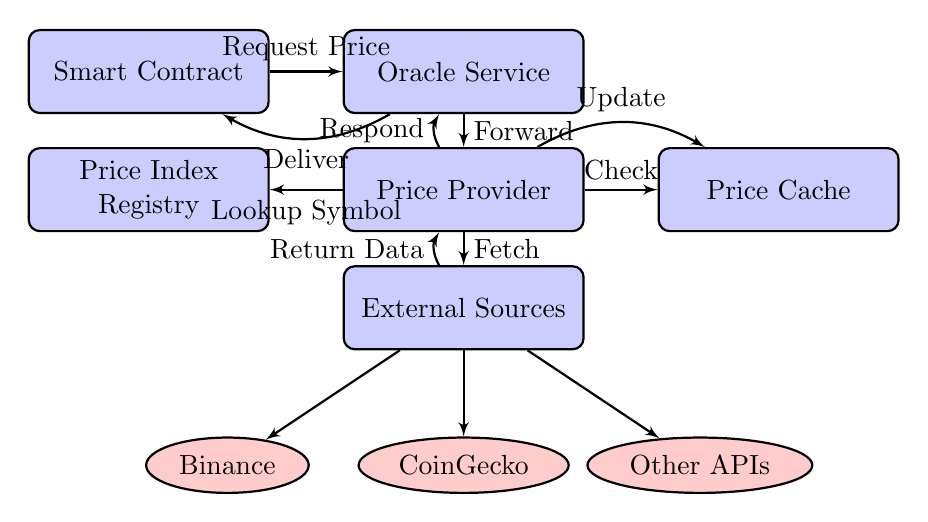
\begin{tikzpicture}[node distance=1.5cm, auto, thick]
    % Define styles
    \tikzstyle{block} = [rectangle, draw, fill=blue!20, text width=8em, text centered, rounded corners, minimum height=3em]
    \tikzstyle{line} = [draw, -latex']
    \tikzstyle{cloud} = [draw, ellipse, fill=red!20, node distance=3cm, minimum height=2em]
    
    % Place nodes
    \node [block] (contract) {Smart Contract};
    \node [block, right of=contract, node distance=4cm] (oracle) {Oracle Service};
    \node [block, below of=oracle] (price) {Price Provider};
    \node [block, left of=price, node distance=4cm] (registry) {Price Index Registry};
    \node [block, right of=price, node distance=4cm] (cache) {Price Cache};
    \node [block, below of=price] (sources) {External Sources};
    \node [cloud, below of=sources, node distance=2cm] (coinGecko) {CoinGecko};
    \node [cloud, left of=coinGecko, node distance=3cm] (binance) {Binance};
    \node [cloud, right of=coinGecko, node distance=3cm] (other) {Other APIs};
    
    % Draw edges
    \path [line] (contract) -- node {Request Price} (oracle);
    \path [line] (oracle) -- node {Forward} (price);
    \path [line] (price) -- node {Lookup Symbol} (registry);
    \path [line] (price) -- node {Check} (cache);
    \path [line] (price) -- node {Fetch} (sources);
    \path [line] (sources) -- node {} (coinGecko);
    \path [line] (sources) -- node {} (binance);
    \path [line] (sources) -- node {} (other);
    \path [line] (sources) to [bend left] node {Return Data} (price);
    \path [line] (price) to [bend left] node {Update} (cache);
    \path [line] (price) to [bend left] node {Respond} (oracle);
    \path [line] (oracle) to [bend left] node {Deliver} (contract);
    
\end{tikzpicture}
\caption{Price Data Feed System in Neo Service Layer}
\label{fig:price-data-feed}
\end{figure}


\paragraph{Price Data Feed System}
The Price Data Feed is one of the most critical components of the Oracle Service, providing reliable and timely price information for various assets. The system employs \textbf{Multi-Source Aggregation} by retrieving price data from multiple sources, including major exchanges (Binance, Coinbase, etc.), aggregation services (CoinGecko, CoinMarketCap), and specialized price feeds, ensuring comprehensive market coverage and resilience against single-source failures. To handle the complexity of asset identification across different platforms, a \textbf{Price Index Registry} serves as a sophisticated mapping system that maintains relationships between different symbol representations across various data sources, ensuring consistent identification of assets regardless of the specific notation used by different providers. Performance optimization is achieved through \textbf{Dynamic Caching} which implements an intelligent caching mechanism that balances data freshness with response time, with cache invalidation strategies tailored to different asset types based on their volatility and trading volume. To maintain data quality, \textbf{Outlier Detection} algorithms identify and filter out anomalous price data that could result from market manipulation, technical issues, or other irregularities, protecting applications from acting on incorrect information. Each price point is assigned a \textbf{Confidence Scoring} based on factors such as source reliability, data recency, and consistency across sources, allowing applications to make informed decisions based on the quality of the price data they receive.

A formal specification of the Price Data Feed protocol is provided in Section \ref{subsec:price-feed-protocol}.

\subsection{Price Data Feed Protocol}
\label{subsec:price-feed-protocol}

The Price Data Feed Protocol defines how price data is collected, aggregated, and provided to smart contracts and applications.

\begin{protocol}[Price Data Collection]
\label{prot:price-data-collection}
\begin{algorithmic}[1]
\Require Asset symbol $S$, Price Provider $P$, Price Registry $R$, Cache $C$
\Ensure Accurate and up-to-date price data is collected and stored

\State \textbf{Symbol Resolution:}
\State $\text{mappings} \gets R.\text{getSymbolMappings}(S)$
\If{$\text{mappings} = \emptyset$}
    \State \Return $\{\text{error}: \text{"Unknown symbol"}\}$
\EndIf

\State \textbf{Cache Check:}
\State $\text{cachedData} \gets C.\text{get}(S)$
\If{$\text{cachedData} \neq \text{null} \land \text{now}() - \text{cachedData}.\text{timestamp} < \text{cachedData}.\text{ttl}$}
    \State \Return $\text{cachedData}.\text{price}$
\EndIf

\State \textbf{Source Selection:}
\State $\text{sources} \gets P.\text{getSourcesForAsset}(S)$
\State $\text{prices} \gets \emptyset$

\State \textbf{Parallel Data Retrieval:}
\For{each $\text{source} \in \text{sources}$ \textbf{in parallel}}
    \State $\text{sourceSymbol} \gets \text{mappings}[\text{source}.\text{name}]$
    \State $\text{rawPrice} \gets \text{source}.\text{fetchPrice}(\text{sourceSymbol})$
    \If{$\text{rawPrice}.\text{success}$}
        \State $\text{prices} \gets \text{prices} \cup \{(\text{source}.\text{name}, \text{rawPrice}.\text{price}, \text{rawPrice}.\text{timestamp}, \text{source}.\text{weight})\}$
    \EndIf
\EndFor

\If{$|\text{prices}| < P.\text{minimumSources}$}
    \State \Return $\{\text{error}: \text{"Insufficient price sources"}, \text{available}: |\text{prices}|\}$
\EndIf

\State \textbf{Outlier Detection:}
\State $\text{validPrices} \gets \text{FilterOutliers}(\text{prices})$

\State \textbf{Price Aggregation:}
\State $\text{aggregatedPrice} \gets \text{AggregateWeightedPrice}(\text{validPrices})$
\State $\text{confidence} \gets \text{CalculateConfidence}(\text{validPrices}, \text{aggregatedPrice})$

\State \textbf{Cache Update:}
\State $\text{ttl} \gets P.\text{getTTLForAsset}(S)$
\State $C.\text{set}(S, \{\text{price}: \text{aggregatedPrice}, \text{timestamp}: \text{now}(), \text{ttl}: \text{ttl}, \text{confidence}: \text{confidence}, \text{sources}: \text{validPrices}\})$

\State \Return $\{\text{price}: \text{aggregatedPrice}, \text{timestamp}: \text{now}(), \text{confidence}: \text{confidence}\}$
\end{algorithmic}
\end{protocol}

\begin{protocol}[Oracle Price Request]
\label{prot:oracle-price-request}
\begin{algorithmic}[1]
\Require Requester $R$, Asset symbol $S$, Callback information $C$, Oracle Service $O$, Price Provider $P$
\Ensure Price data is delivered to the requester through the specified callback mechanism

\State \textbf{Request Validation:}
\State $\text{valid} \gets \text{ValidateRequest}(R, S, C)$
\If{$\neg \text{valid}$}
    \State \Return $\{\text{error}: \text{"Invalid request"}\}$
\EndIf

\State \textbf{Request Registration:}
\State $\text{requestId} \gets \text{GenerateUniqueID}()$
\State $O.\text{registerRequest}(\text{requestId}, R, S, C)$

\State \textbf{Price Collection:}
\State $\text{priceResult} \gets P.\text{collectPrice}(S)$
\If{$\text{priceResult}.\text{error} \neq \text{null}$}
    \State $O.\text{updateRequestStatus}(\text{requestId}, \text{"failed"}, \text{priceResult}.\text{error})$
    \If{$C.\text{type} = \text{"blockchain"}$}
        \State $O.\text{sendErrorCallback}(C.\text{contract}, C.\text{method}, \text{requestId}, \text{priceResult}.\text{error})$
    \ElsIf{$C.\text{type} = \text{"http"}$}
        \State $O.\text{sendHttpErrorResponse}(C.\text{url}, \text{requestId}, \text{priceResult}.\text{error})$
    \EndIf
    \State \Return $\{\text{error}: \text{priceResult}.\text{error}, \text{requestId}: \text{requestId}\}$
\EndIf

\State \textbf{Response Signing:}
\State $\text{response} \gets \{\text{requestId}: \text{requestId}, \text{symbol}: S, \text{price}: \text{priceResult}.\text{price}, \text{timestamp}: \text{priceResult}.\text{timestamp}, \text{confidence}: \text{priceResult}.\text{confidence}\}$
\State $\text{signature} \gets O.\text{signResponse}(\text{response})$
\State $\text{signedResponse} \gets \{\text{response}: \text{response}, \text{signature}: \text{signature}\}$

\State \textbf{Callback Execution:}
\If{$C.\text{type} = \text{"blockchain"}$}
    \State $\text{tx} \gets O.\text{createCallbackTransaction}(C.\text{contract}, C.\text{method}, \text{signedResponse})$
    \State $\text{txHash} \gets O.\text{submitTransaction}(\text{tx})$
    \State $O.\text{monitorTransaction}(\text{txHash})$
\ElsIf{$C.\text{type} = \text{"http"}$}
    \State $O.\text{sendHttpResponse}(C.\text{url}, \text{signedResponse})$
\EndIf

\State \textbf{Request Completion:}
\State $O.\text{updateRequestStatus}(\text{requestId}, \text{"completed"}, \text{signedResponse})$

\State \Return $\{\text{success}: \text{true}, \text{requestId}: \text{requestId}, \text{response}: \text{signedResponse}\}$
\end{algorithmic}
\end{protocol}


\paragraph{Oracle Request Processing Protocol}
The Oracle Service implements a comprehensive protocol for processing requests that ensures reliability, security, and efficiency. The process begins with \textbf{Request Validation}, where incoming requests are thoroughly validated for proper formatting, parameter completeness, and requester authorization to prevent malformed or unauthorized requests from entering the system. Once validated, \textbf{Request Classification} categorizes requests by type and priority to ensure appropriate handling and resource allocation, allowing critical requests to be processed with higher priority. The system then performs \textbf{Source Selection}, where based on the request type and parameters, appropriate data sources are selected from the available provider pool, considering factors such as reliability, specialization, and historical performance. To optimize performance, \textbf{Parallel Data Retrieval} is employed, retrieving data from multiple sources simultaneously to minimize latency and ensure redundancy in case any individual source fails. The collected data undergoes \textbf{Data Aggregation} using appropriate algorithms such as median, volume-weighted average, or other statistical methods based on the data type, producing a consensus result that mitigates outliers and anomalies. Before delivery, \textbf{Result Verification} checks the aggregated results against predefined validity criteria and historical patterns to detect potential errors or manipulation. For security, \textbf{Response Signing} cryptographically signs the final result to ensure its authenticity and integrity, allowing recipients to verify its origin. The system then handles \textbf{Response Delivery}, where the signed result is delivered to the requester through the specified callback mechanism or stored for retrieval, with support for various delivery methods including blockchain transactions, API callbacks, and message queues. For blockchain-based callbacks, \textbf{Transaction Confirmation} monitors the transaction until confirmation, ensuring that the data is successfully recorded on-chain. Finally, \textbf{Request Archiving} stores request details and results for audit, dispute resolution, and performance analysis, creating a comprehensive record of all oracle operations.

\paragraph{Blockchain Gateway Integration}
The Oracle Service integrates with blockchain networks through specialized gateways that enable seamless interaction with different blockchain ecosystems. The \textbf{Neo N3 Gateway} provides native integration with the Neo N3 blockchain, supporting direct interaction with NeoContract smart contracts through optimized interfaces that leverage Neo's unique features and capabilities. For projects operating on Ethereum or its derivatives, the \textbf{Ethereum Gateway} offers integration with Ethereum and EVM-compatible chains, supporting interaction with Solidity smart contracts through standardized interfaces that comply with Ethereum's design patterns and conventions. To address the growing need for cross-chain functionality, the service includes a \textbf{Cross-Chain Oracle} with specialized components that enable oracle data to be used across multiple blockchain networks, maintaining consistency and reliability through sophisticated synchronization and verification mechanisms that ensure data integrity across different consensus systems.

\subsubsection{Event Messaging System}
\label{subsubsec:event-messaging}

The Event Messaging System is a core component of the Neo Service Layer that enables asynchronous communication between different parts of the platform. It provides a reliable and scalable mechanism for detecting, processing, and responding to events from various sources, including the Neo N3 blockchain, external systems, and internal services.

\begin{figure}[h]
\centering
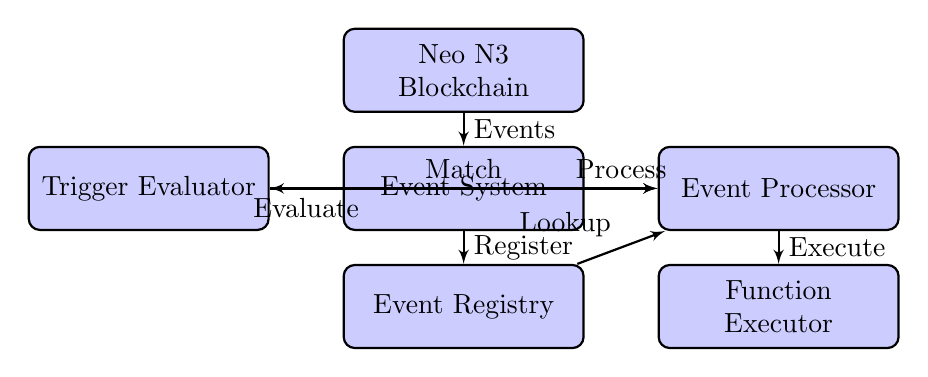
\begin{tikzpicture}[node distance=1.5cm, auto, thick]
    % Define styles
    \tikzstyle{block} = [rectangle, draw, fill=blue!20, text width=8em, text centered, rounded corners, minimum height=3em]
    \tikzstyle{line} = [draw, -latex']
    \tikzstyle{cloud} = [draw, ellipse, fill=red!20, node distance=3cm, minimum height=2em]
    
    % Place nodes
    \node [block] (blockchain) {Neo N3 Blockchain};
    \node [block, below of=blockchain] (event) {Event System};
    \node [block, below of=event] (registry) {Event Registry};
    \node [block, left of=event, node distance=4cm] (trigger) {Trigger Evaluator};
    \node [block, right of=event, node distance=4cm] (processor) {Event Processor};
    \node [block, below of=processor] (function) {Function Executor};
    
    % Draw edges
    \path [line] (blockchain) -- node {Events} (event);
    \path [line] (event) -- node {Register} (registry);
    \path [line] (event) -- node {Evaluate} (trigger);
    \path [line] (trigger) -- node {Match} (processor);
    \path [line] (event) -- node {Process} (processor);
    \path [line] (processor) -- node {Execute} (function);
    \path [line] (registry) -- node {Lookup} (processor);
    
\end{tikzpicture}
\caption{Neo Service Layer Event Messaging System}
\label{fig:event-messaging}
\end{figure}


\begin{definition}[Event]
An Event is a discrete occurrence or notification that represents a change in state or a significant action within the system. Each event has:
\begin{itemize}
    \item Type: The category of the event (blockchain, system, custom)
    \item Source: The origin of the event
    \item Payload: The data associated with the event
    \item Timestamp: When the event occurred
    \item ID: A unique identifier for the event
\end{itemize}
\end{definition}

The Event Messaging System consists of several key components that work together to provide a comprehensive event processing pipeline. \textbf{Event Sources} serve as connectors that monitor and capture events from various origins, including blockchain networks, external APIs, and internal services, providing the raw event data that enters the system. The \textbf{Event Registry} functions as a centralized repository that maintains information about event types, their schemas, and associated triggers, ensuring that events are properly categorized and matched with appropriate handlers. When events enter the system, the \textbf{Trigger Evaluator} evaluates them against registered triggers to determine which functions should be executed in response, applying complex matching rules and conditions to ensure precise function selection. Once triggers are matched, the \textbf{Event Processor} handles events by enriching them with additional context and routing them to the appropriate handlers, transforming raw events into actionable information. Finally, the \textbf{Function Executor} executes the functions triggered by events, managing their lifecycle from initialization to completion and handling their results, which may include storing data, sending notifications, or triggering additional events.

\paragraph{Event Processing Protocol}
The Event Messaging System implements a comprehensive protocol for processing events that ensures reliable and efficient event handling. The process begins with \textbf{Event Detection}, where specialized monitors observe various sources such as blockchain networks, message queues, and system components to identify relevant events as they occur. Once detected, \textbf{Event Validation} checks these events against their schema definitions to ensure they contain all required fields and conform to the expected format, preventing malformed events from entering the processing pipeline. To enhance the event's utility, \textbf{Event Enrichment} adds additional context such as related data from other systems, historical information, or derived attributes, creating a more comprehensive event representation. The enriched events undergo \textbf{Trigger Matching}, where they are compared against registered triggers using pattern matching, condition evaluation, and other criteria to determine which actions should be taken in response. When a trigger matches an event, \textbf{Function Selection} identifies the associated functions that should be executed, creating a mapping between events and their handlers. Before execution, \textbf{Execution Planning} determines the optimal execution order, parallelization strategy, and resource allocation for the selected functions, ensuring efficient processing. The system then performs \textbf{Function Invocation}, where selected functions are called with the event data and any additional context required for processing, executing the business logic associated with the event. After execution, \textbf{Result Handling} processes the function results, which may include storing data, sending notifications, or triggering additional events, creating a chain of event-driven actions. Finally, \textbf{Event Archiving} stores processed events and their handling results for auditing, analytics, and debugging purposes, creating a comprehensive record of system activity.

A formal specification of the event processing protocol is provided in Section \ref{subsec:event-protocol}.

\subsection{Event Messaging Protocol}
\label{subsec:event-messaging-protocol}

The Event Messaging Protocol defines how events are detected, processed, and routed to appropriate handlers.

\begin{tcolorbox}[
    enhanced,
    colback=blue!5!white,
    colframe=blue!75!black,
    arc=5mm,
    boxrule=1.5pt,
    title=Event Processing Protocol,
    fonttitle=\bfseries,
    coltitle=white,
    attach boxed title to top left={yshift=-2mm, xshift=5mm},
    boxed title style={colback=blue!75!black, rounded corners},
    shadow={2mm}{-2mm}{0mm}{black!50},
    drop fuzzy shadow
]
\begin{tcolorbox}[
    enhanced,
    colback=blue!5!white,
    colframe=blue!75!black,
    arc=5mm,
    boxrule=1.5pt,
    title=Protocol,
    fonttitle=\bfseries,
    coltitle=white,
    attach boxed title to top left={yshift=-2mm, xshift=5mm},
    boxed title style={colback=blue!75!black, rounded corners},
    shadow={2mm}{-2mm}{0mm}{black!50},
    drop fuzzy shadow
]
\begin{protocol}{Event Processing}
\label{prot:event-processing}
\begin{algorithmic}[1]
\Require Event source $S$, Event registry $R$, Trigger evaluator $T$, Function registry $F$
\Ensure Proper event processing and function execution

\State \textbf{Event Detection:}
\State $e \gets \text{DetectEvent}(S)$ \Comment{Detect event from source}
\State $\text{valid} \gets \text{ValidateEvent}(e, \text{schema}(e.\text{type}))$
\If{$\neg \text{valid}$}
    \State \textbf{reject} $e$
\EndIf

\State \textbf{Event Enrichment:}
\State $e' \gets \text{EnrichEvent}(e, \text{context}(e))$ \Comment{Add context information}

\State \textbf{Trigger Matching:}
\State $\text{triggers} \gets \emptyset$
\For{each $t \in R.\text{getTriggers}(e'.\text{type})$}
    \If{$\text{EvaluateTrigger}(t, e')$}
        \State $\text{triggers} \gets \text{triggers} \cup \{t\}$
    \EndIf
\EndFor

\State \textbf{Function Selection:}
\State $\text{functions} \gets \emptyset$
\For{each $t \in \text{triggers}$}
    \State $\text{functions} \gets \text{functions} \cup F.\text{getFunctions}(t)$
\EndFor

\State \textbf{Execution Planning:}
\State $\text{plan} \gets \text{CreateExecutionPlan}(\text{functions}, e')$

\State \textbf{Function Execution:}
\For{each $f \in \text{plan}.\text{getOrderedFunctions}()$}
    \State $\text{result}_f \gets \text{ExecuteFunction}(f, e', \text{context}(f))$
    \State $\text{ProcessResult}(\text{result}_f, f, e')$
\EndFor

\State \textbf{Event Archiving:}
\State $\text{ArchiveEvent}(e', \text{triggers}, \text{functions}, \{\text{result}_f\})$
\end{algorithmic}
\end{protocol}
\end{tcolorbox}



\paragraph{Blockchain Event Integration}
The Event Messaging System provides specialized integration with the Neo N3 blockchain through a comprehensive set of event types that capture different aspects of blockchain activity. The system processes \textbf{Block Events} which provide notifications for new blocks, including block height, timestamp, and transaction count, enabling applications to track blockchain progression and synchronize with the latest state. For transaction monitoring, \textbf{Transaction Events} deliver notifications for transactions, including transaction hash, sender, receiver, and amount, allowing applications to track fund movements and transaction confirmations in real-time. Smart contract interactions are captured through \textbf{Contract Events} which provide notifications for smart contract events, including contract hash, event name, and parameters, enabling applications to respond to specific contract state changes and user interactions. The system also monitors \textbf{State Changes} with notifications for modifications to the blockchain state, such as balance updates, contract deployments, and storage modifications, providing a comprehensive view of the evolving blockchain ecosystem.

\paragraph{Event Filtering and Routing}
The system provides sophisticated filtering and routing capabilities that enable precise control over event processing flows. \textbf{Content-Based Filtering} allows events to be filtered based on their content, such as specific field values or patterns, enabling applications to focus on only the most relevant events for their use case. For more dynamic routing decisions, \textbf{Context-Based Routing} directs events to different handlers based on contextual information such as user identity, application, or environment, creating adaptive processing pipelines that can respond to changing conditions. The system implements \textbf{Priority-Based Processing} where events can be assigned priorities that determine their processing order and resource allocation, ensuring that critical events are handled promptly even during high load periods. To protect system stability and ensure fair resource distribution, \textbf{Rate Limiting} mechanisms can be applied to event processing, preventing any single source or event type from overwhelming the system while maintaining responsiveness for all applications.

\subsubsection{Function Deployment and Execution}
\label{subsubsec:function-deployment}

The Neo Service Layer provides a comprehensive system for deploying, managing, and executing serverless functions. This system enables developers to create and deploy code that responds to events, processes data, and interacts with blockchain networks without managing the underlying infrastructure.

\begin{figure}[h]
\centering
\begin{tcolorbox}[
    enhanced,
    colback=blue!5!white,
    colframe=blue!75!black,
    arc=5mm,
    boxrule=1.5pt,
    title=Function Deployment Process,
    fonttitle=\bfseries,
    coltitle=white,
    attach boxed title to top left={yshift=-2mm, xshift=5mm},
    boxed title style={colback=blue!75!black, rounded corners},
    shadow={2mm}{-2mm}{0mm}{black!50},
    drop fuzzy shadow
]
\begin{tikzpicture}[node distance=1.5cm, auto]
    % Define styles
    \tikzstyle{block} = [rectangle, draw, fill=blue!20, text width=8em, text centered, rounded corners, minimum height=3em]
    \tikzstyle{line} = [draw, -latex']
    \tikzstyle{cloud} = [draw, ellipse, fill=red!20, node distance=3cm, minimum height=2em]
    
    % Place nodes
    \node [block] (developer) {Developer};
    \node [block, right=of developer] (cli) {CLI/API};
    \node [block, right=of cli] (registry) {Function Registry};
    \node [block, below=of registry] (storage) {Function Storage};
    \node [block, below=of cli] (worker) {Worker Nodes};
    
    % Draw edges
    \path [line] (developer) -- node[above-arrow-text] {1. Submit Code} (cli);
    \path [line] (cli) -- node[above-arrow-text] {2. Validate} (registry);
    \path [line] (registry) -- node[above-arrow-text] {3. Store} (storage);
    \path [line] (registry) -- node[above-arrow-text, left] {4. Notify} (worker);
    \path [line] (worker) -- node[above-arrow-text] {5. Load Function} (storage);
\end{tikzpicture}
\end{tcolorbox}
\caption{Function Deployment Process Flow}
\label{fig:function-deployment}
\end{figure}


\begin{definition}[Function]
A Function is a unit of code that performs a specific task when invoked. Each function has:
\begin{itemize}
    \item Name: A unique identifier for the function
    \item Code: The executable code that implements the function logic
    \item Runtime: The environment in which the function executes (e.g., JavaScript, TypeScript)
    \item Configuration: Settings that control the function's behavior and resource allocation
    \item Triggers: Conditions that cause the function to be executed
    \item Permissions: Access controls that determine what resources the function can use
\end{itemize}
\end{definition}

\paragraph{Function Deployment Process}
The deployment process involves several interconnected steps to ensure functions are properly registered, stored, and made available for execution. The process begins with \textbf{Function Submission}, where developers submit functions through the API Service, providing the function code, configuration, and metadata necessary for deployment. Once submitted, \textbf{Code Validation} thoroughly checks the code for syntax correctness, security vulnerabilities, and compliance with platform policies, ensuring that only secure and well-formed functions enter the system. For functions with external dependencies, \textbf{Dependency Resolution} identifies, validates, and prepares any required dependencies for inclusion in the execution environment, ensuring that functions have access to all necessary libraries and resources. The function is then formally added to the system through \textbf{Function Registration} in the Function Registry, which maintains comprehensive information about all available functions, including their interfaces, permissions, and metadata. For persistent storage, the \textbf{Storage} step securely saves the function code and configuration in the Storage System, which provides durable and versioned storage with rollback capabilities. To enable event-driven execution, \textbf{Trigger Registration} records any triggers associated with the function in the Event Registry, enabling event-based invocation when specified conditions are met. Finally, \textbf{Distribution} deploys the function to Worker Nodes, which prepare the execution environment and cache the function for efficient invocation, optimizing performance by reducing cold-start times.

A formal specification of the function deployment and execution protocol is provided in Section \ref{subsec:function-protocol}.

\subsection{Function Deployment and Execution Protocol}
\label{subsec:function-protocol}

The Function Deployment and Execution Protocol defines how functions are deployed, managed, and executed within the Neo Service Layer.

\begin{tcolorbox}[
    enhanced,
    colback=blue!5!white,
    colframe=blue!75!black,
    arc=5mm,
    boxrule=1.5pt,
    title=Function Deployment Protocol,
    fonttitle=\bfseries,
    coltitle=white,
    attach boxed title to top left={yshift=-2mm, xshift=5mm},
    boxed title style={colback=blue!75!black, rounded corners},
    shadow={2mm}{-2mm}{0mm}{black!50},
    drop fuzzy shadow
]
\begin{tcolorbox}[
    enhanced,
    colback=blue!5!white,
    colframe=blue!75!black,
    arc=5mm,
    boxrule=1.5pt,
    title=Function Protocol,
    fonttitle=\bfseries,
    coltitle=white,
    attach boxed title to top left={yshift=-2mm, xshift=5mm},
    boxed title style={colback=blue!75!black, rounded corners},
    shadow={2mm}{-2mm}{0mm}{black!50},
    drop fuzzy shadow
]
\begin{tcolorbox}[
    enhanced,
    colback=blue!5!white,
    colframe=blue!75!black,
    arc=5mm,
    boxrule=1.5pt,
    title=Protocol,
    fonttitle=\bfseries,
    coltitle=white,
    attach boxed title to top left={yshift=-2mm, xshift=5mm},
    boxed title style={colback=blue!75!black, rounded corners},
    shadow={2mm}{-2mm}{0mm}{black!50},
    drop fuzzy shadow
]
\begin{protocol}{Function Deployment}
\label{prot:function-deployment}
\begin{algorithmic}[1]
\Require Function code $C$, Configuration $\text{conf}$, Metadata $M$, Function Registry $R$, Storage System $S$
\Ensure Function is properly deployed and available for execution

\State \textbf{Function Submission:}
\State $F \gets \{\text{code}: C, \text{config}: \text{conf}, \text{metadata}: M\}$

\State \textbf{Code Validation:}
\State $\text{valid} \gets \text{ValidateCode}(F.\text{code})$
\If{$\neg \text{valid}$}
    \State \textbf{reject} $F$
\EndIf

\State \textbf{Dependency Resolution:}
\State $\text{deps} \gets \text{ResolveDependencies}(F.\text{code}, F.\text{config})$
\State $F.\text{dependencies} \gets \text{deps}$

\State \textbf{Function Registration:}
\State $\text{id} \gets \text{GenerateUniqueID}(F.\text{metadata}.\text{name})$
\State $F.\text{id} \gets \text{id}$
\State $R.\text{registerFunction}(F)$

\State \textbf{Storage:}
\State $S.\text{storeFunction}(F)$

\State \textbf{Trigger Registration:}
\For{each $t \in F.\text{config}.\text{triggers}$}
    \State $\text{EventRegistry}.\text{registerTrigger}(t, F.\text{id})$
\EndFor

\State \textbf{Distribution:}
\For{each $\text{node} \in \text{WorkerNodes}$}
    \State $\text{DistributeFunction}(F, \text{node})$
\EndFor

\State \Return $F.\text{id}$
\end{algorithmic}
\end{protocol}
\end{tcolorbox}



\begin{tcolorbox}[
    enhanced,
    colback=blue!5!white,
    colframe=blue!75!black,
    arc=5mm,
    boxrule=1.5pt,
    title=Function Execution Protocol,
    fonttitle=\bfseries,
    coltitle=white,
    attach boxed title to top left={yshift=-2mm, xshift=5mm},
    boxed title style={colback=blue!75!black, rounded corners},
    shadow={2mm}{-2mm}{0mm}{black!50},
    drop fuzzy shadow
]
\begin{tcolorbox}[
    enhanced,
    colback=blue!5!white,
    colframe=blue!75!black,
    arc=5mm,
    boxrule=1.5pt,
    title=Function Protocol,
    fonttitle=\bfseries,
    coltitle=white,
    attach boxed title to top left={yshift=-2mm, xshift=5mm},
    boxed title style={colback=blue!75!black, rounded corners},
    shadow={2mm}{-2mm}{0mm}{black!50},
    drop fuzzy shadow
]
\begin{tcolorbox}[
    enhanced,
    colback=blue!5!white,
    colframe=blue!75!black,
    arc=5mm,
    boxrule=1.5pt,
    title=Protocol,
    fonttitle=\bfseries,
    coltitle=white,
    attach boxed title to top left={yshift=-2mm, xshift=5mm},
    boxed title style={colback=blue!75!black, rounded corners},
    shadow={2mm}{-2mm}{0mm}{black!50},
    drop fuzzy shadow
]
\begin{protocol}{Function Execution}
\label{prot:function-execution}
\begin{algorithmic}[1]
\Require Function ID $\text{id}$, Input data $D$, Context $\text{ctx}$, Scheduler $\text{sched}$, Worker Nodes $W$
\Ensure Function is executed securely and results are properly handled

\State \textbf{Function Lookup:}
\State $F \gets \text{FunctionRegistry}.\text{getFunction}(\text{id})$

\State \textbf{Worker Assignment:}
\State $\text{worker} \gets \text{sched}.\text{assignWorker}(F, D, \text{ctx})$

\State \textbf{Resource Allocation:}
\State $\text{resources} \gets \text{worker}.\text{allocateResources}(F.\text{config}.\text{resources})$

\State \textbf{Sandbox Creation:}
\State $\text{sandbox} \gets \text{worker}.\text{createSandbox}(\text{resources})$

\State \textbf{Runtime Initialization:}
\State $\text{runtime} \gets \text{sandbox}.\text{initializeRuntime}(F.\text{config}.\text{runtime})$
\State $\text{runtime}.\text{setPermissions}(F.\text{config}.\text{permissions})$

\State \textbf{Function Loading:}
\State $\text{runtime}.\text{loadFunction}(F.\text{code}, F.\text{dependencies})$

\State \textbf{Execution:}
\State $\text{result} \gets \text{runtime}.\text{executeFunction}(F.\text{metadata}.\text{entrypoint}, D, \text{ctx})$

\State \textbf{Monitoring:}
\While{$\text{runtime}.\text{isExecuting}()$}
    \State $\text{metrics} \gets \text{runtime}.\text{getMetrics}()$
    \If{$\text{metrics}.\text{exceedsLimits}(F.\text{config}.\text{limits})$}
        \State $\text{runtime}.\text{terminate}()$
        \State \Return $\{\text{error}: \text{"Resource limits exceeded"}\}$
    \EndIf
\EndWhile

\State \textbf{Result Capture:}
\State $\text{output} \gets \text{runtime}.\text{getOutput}()$
\State $\text{errors} \gets \text{runtime}.\text{getErrors}()$
\State $\text{logs} \gets \text{runtime}.\text{getLogs}()$

\State \textbf{Resource Cleanup:}
\State $\text{sandbox}.\text{cleanup}()$
\State $\text{worker}.\text{releaseResources}(\text{resources})$

\State \textbf{Result Processing:}
\State $\text{ProcessFunctionResult}(\text{output}, \text{errors}, \text{logs}, F, D, \text{ctx})$

\State \Return $\{\text{output}: \text{output}, \text{errors}: \text{errors}, \text{logs}: \text{logs}\}$
\end{algorithmic}
\end{protocol}
\end{tcolorbox}




\begin{figure}[h]
\centering
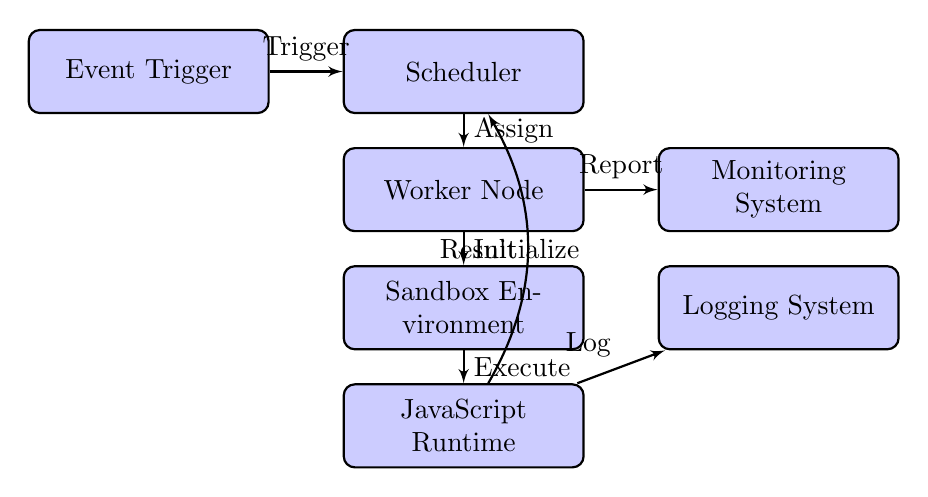
\begin{tikzpicture}[node distance=1.5cm, auto, thick]
    % Define styles
    \tikzstyle{block} = [rectangle, draw, fill=blue!20, text width=8em, text centered, rounded corners, minimum height=3em]
    \tikzstyle{line} = [draw, -latex']
    \tikzstyle{cloud} = [draw, ellipse, fill=red!20, node distance=3cm, minimum height=2em]
    
    % Place nodes
    \node [block] (event) {Event Trigger};
    \node [block, right of=event, node distance=4cm] (scheduler) {Scheduler};
    \node [block, below of=scheduler] (worker) {Worker Node};
    \node [block, below of=worker] (sandbox) {Sandbox Environment};
    \node [block, below of=sandbox] (runtime) {JavaScript Runtime};
    \node [block, right of=worker, node distance=4cm] (monitor) {Monitoring System};
    \node [block, below of=monitor] (logger) {Logging System};
    
    % Draw edges
    \path [line] (event) -- node {Trigger} (scheduler);
    \path [line] (scheduler) -- node {Assign} (worker);
    \path [line] (worker) -- node {Initialize} (sandbox);
    \path [line] (sandbox) -- node {Execute} (runtime);
    \path [line] (worker) -- node {Report} (monitor);
    \path [line] (runtime) -- node {Log} (logger);
    \path [line] (runtime) to [bend right] node {Result} (scheduler);
    
\end{tikzpicture}
\caption{Function Execution Flow in Neo Service Layer}
\label{fig:function-execution}
\end{figure}


\paragraph{Function Execution Flow}
When a function is triggered for execution, the system follows a comprehensive flow to ensure reliable and secure processing. The process begins with \textbf{Trigger Evaluation}, where an event or direct invocation initiates the function execution process, determining which function needs to be executed and with what parameters. Once triggered, \textbf{Scheduler Assignment} occurs, where the Scheduler assigns the function execution task to an appropriate Worker Node based on factors such as load, locality, and resource requirements, optimizing resource utilization across the platform. The selected Worker Node then undergoes \textbf{Worker Preparation}, allocating resources and initializing the execution environment to ensure it has sufficient capacity to handle the function. For security, \textbf{Sandbox Creation} establishes a secure sandbox environment to isolate the function execution from other functions and the host system, preventing potential security breaches or resource conflicts. Within this sandbox, \textbf{Runtime Initialization} prepares the JavaScript runtime (based on Deno Core) with appropriate permissions and API access, creating a controlled execution context with precisely defined capabilities. The system then performs \textbf{Function Loading}, where the function code and dependencies are loaded into the runtime environment, making them available for execution. The core step of \textbf{Execution} runs the function with the provided input data and context, executing the business logic defined by the developer. During execution, \textbf{Monitoring} tracks resource usage, execution time, and other metrics to ensure compliance with limits and detect anomalies, preventing runaway processes or resource exhaustion. After execution completes, \textbf{Result Capture} collects the function's output, including return values, errors, and side effects, providing comprehensive information about the execution outcome. The system then performs \textbf{Resource Cleanup}, releasing resources and cleaning up or recycling the sandbox environment to maintain system efficiency. Finally, \textbf{Result Processing} handles the execution results according to the function configuration, which may include storing data, sending notifications, or triggering additional functions, creating chains of function executions that can implement complex workflows.

\paragraph{Resource Management}
The function execution system implements sophisticated resource management to ensure efficient and fair allocation across all functions and applications. The system enforces \textbf{CPU Limits} by allocating specific CPU quotas to functions, preventing excessive usage by any single function and ensuring fair sharing of computational resources across all workloads. To prevent memory-related issues, \textbf{Memory Allocation} is carefully monitored and limited to prevent memory leaks and excessive consumption, ensuring system stability even under high load conditions. For operational safety, \textbf{Execution Timeouts} are implemented where functions have maximum execution time limits to prevent infinite loops and resource hogging, automatically terminating functions that exceed their allocated time. The platform optimizes overall throughput through \textbf{Concurrency Control}, managing the number of concurrent function executions to balance responsiveness with system stability, preventing overload while maximizing resource utilization. To adapt to changing demand patterns, \textbf{Auto-scaling} capabilities allow Worker Nodes to be dynamically scaled based on demand, automatically adding resources during peak periods and reducing them during low-demand periods to handle varying workloads efficiently while optimizing operational costs.

\subsubsection{Secret Storage and Management}
\label{subsubsec:secret-storage}

The Secret Storage and Management system provides a secure way for functions to store and access sensitive information such as API keys, credentials, and private keys. This system ensures that secrets are protected from unauthorized access while remaining available to authorized functions.

\begin{figure}[h]
\centering
\begin{tcolorbox}[
    enhanced,
    colback=blue!5!white,
    colframe=blue!75!black,
    arc=5mm,
    boxrule=1.5pt,
    title=Secret Storage Architecture,
    fonttitle=\bfseries,
    coltitle=white,
    attach boxed title to top left={yshift=-2mm, xshift=5mm},
    boxed title style={colback=blue!75!black, rounded corners},
    shadow={2mm}{-2mm}{0mm}{black!50},
    drop fuzzy shadow
]
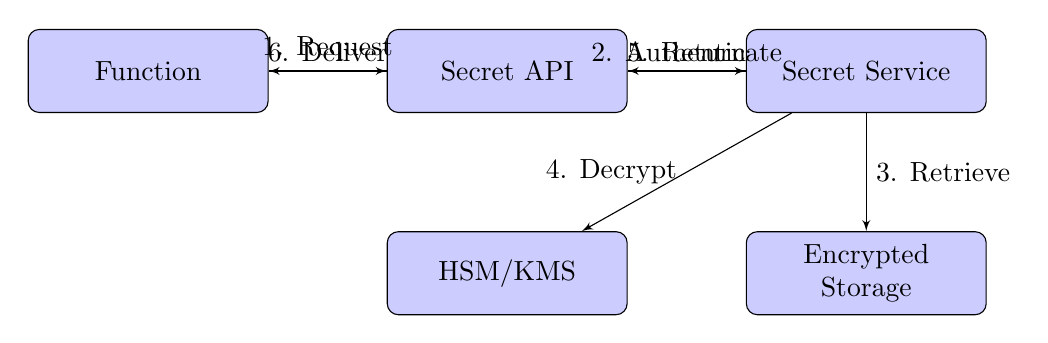
\begin{tikzpicture}[node distance=1.5cm, auto]
    % Define styles
    \tikzstyle{block} = [rectangle, draw, fill=blue!20, text width=8em, text centered, rounded corners, minimum height=3em]
    \tikzstyle{line} = [draw, -latex']
    \tikzstyle{cloud} = [draw, ellipse, fill=red!20, node distance=3cm, minimum height=2em]
    
    % Place nodes
    \node [block] (function) {Function};
    \node [block, right=of function] (api) {Secret API};
    \node [block, right=of api] (service) {Secret Service};
    \node [block, below=of service] (storage) {Encrypted Storage};
    \node [block, below=of api] (hsm) {HSM/KMS};
    
    % Draw edges
    \path [line] (function) -- node {1. Request} (api);
    \path [line] (api) -- node {2. Authenticate} (service);
    \path [line] (service) -- node {3. Retrieve} (storage);
    \path [line] (service) -- node [left] {4. Decrypt} (hsm);
    \path [line] (service) -- node [above] {5. Return} (api);
    \path [line] (api) -- node [above] {6. Deliver} (function);
\end{tikzpicture}
\end{tcolorbox}
\caption{Secret Storage Architecture and Access Flow}
\label{fig:secret-storage}
\end{figure}


\begin{definition}[Secret]
A Secret is a piece of sensitive information that requires protection from unauthorized access. Each secret has:
\begin{itemize}
    \item Key: A unique identifier for the secret
    \item Value: The sensitive data being stored
    \item Owner: The entity that controls access to the secret
    \item Permissions: Rules that determine which functions can access the secret
    \item Metadata: Additional information about the secret, such as creation time and expiration
\end{itemize}
\end{definition}

\paragraph{Secret Storage Architecture}
The Secret Storage system implements a multi-layered architecture to ensure comprehensive security throughout the secret management lifecycle. At the front end, the \textbf{API Layer} provides a standardized interface for functions to store, retrieve, and manage secrets, offering a consistent and secure access point for all secret operations. Behind this interface, the \textbf{Service Layer} implements the core logic for secret management, including access control, encryption, and lifecycle management, coordinating the various components involved in secret handling. For data protection, the \textbf{Encryption Layer} ensures that all secrets are encrypted at rest using strong cryptographic algorithms, preventing unauthorized access even if the underlying storage is compromised. The \textbf{Storage Layer} provides durable and reliable storage for encrypted secrets, ensuring that secrets remain available and intact even in the face of system failures. Throughout the system, \textbf{Access Control} mechanisms enforce permissions and policies that determine who can access which secrets, implementing the principle of least privilege to minimize potential security risks. For security monitoring and compliance, comprehensive \textbf{Audit Logging} records all access attempts and operations, creating an immutable trail of all interactions with the secret storage system that can be used for security analysis and regulatory compliance.

\paragraph{Secret Management Protocol}
The system implements a comprehensive protocol for managing secrets throughout their lifecycle, ensuring security at every stage. The process begins with \textbf{Secret Creation}, where a new secret is assigned a unique identifier, encrypted with a master key, and stored in the storage layer, establishing the foundation for secure secret management. Following creation, \textbf{Access Control Configuration} allows the owner to define precise access permissions, specifying which functions or users can access the secret, implementing the principle of least privilege. When a function requires access to a secret, \textbf{Secret Retrieval} is initiated, where the function sends a request to the Secret API with its authentication credentials, initiating the secure access process. Upon receiving a request, the system performs an \textbf{Authorization Check}, verifying that the requesting function has permission to access the requested secret, preventing unauthorized access attempts. For authorized requests, \textbf{Decryption} occurs where the service retrieves the encrypted secret from storage, decrypts it using the master key, and returns it to the function, ensuring that secrets are only exposed to authorized entities. To maintain a comprehensive audit trail, \textbf{Usage Tracking} logs all access to secrets, including the requester, timestamp, and operation, providing visibility into secret usage patterns and potential security incidents. To minimize the risk of long-term compromise, \textbf{Secret Rotation} automatically updates secrets according to configured policies, ensuring that even if a secret is compromised, the window of vulnerability is limited. In cases of suspected compromise, \textbf{Secret Revocation} provides immediate invalidation of secrets, preventing further access and mitigating potential damage from unauthorized use.

A formal specification of the secret management protocol is provided in Section \ref{subsec:secret-protocol}.

\subsection{Secret Storage and Management Protocol}
\label{subsec:secret-protocol}

The Secret Storage and Management Protocol defines how sensitive information is securely stored, accessed, and managed within the Neo Service Layer.

\begin{protocol}[Secret Storage]
\label{prot:secret-storage}
\begin{algorithmic}[1]
\Require Secret key $k$, Secret value $v$, Owner $o$, Permissions $P$, Secret Service $S$
\Ensure Secret is securely stored and accessible only to authorized entities

\State \textbf{Secret Creation:}
\State $\text{metadata} \gets \{\text{created}: \text{now}(), \text{owner}: o, \text{permissions}: P\}$
\State $\text{secret} \gets \{k, v, \text{metadata}\}$

\State \textbf{Access Control Setup:}
\State $\text{acl} \gets \text{CreateAccessControlList}(o, P)$
\State $S.\text{registerACL}(k, \text{acl})$

\State \textbf{Encryption:}
\State $\text{dataKey} \gets \text{GenerateDataKey}()$
\State $\text{encryptedValue} \gets \text{Encrypt}(v, \text{dataKey})$
\State $\text{encryptedDataKey} \gets \text{Encrypt}(\text{dataKey}, S.\text{masterKey})$

\State \textbf{Storage:}
\State $\text{record} \gets \{k, \text{encryptedValue}, \text{encryptedDataKey}, \text{metadata}\}$
\State $S.\text{storage}.\text{store}(\text{record})$

\State \Return $k$
\end{algorithmic}
\end{protocol}

\begin{protocol}[Secret Retrieval]
\label{prot:secret-retrieval}
\begin{algorithmic}[1]
\Require Secret key $k$, Requester $r$, Secret Service $S$
\Ensure Secret is only provided to authorized requesters

\State \textbf{Authentication:}
\State $\text{authenticated} \gets \text{AuthenticateRequester}(r)$
\If{$\neg \text{authenticated}$}
    \State \textbf{reject} request
\EndIf

\State \textbf{Authorization:}
\State $\text{acl} \gets S.\text{getACL}(k)$
\State $\text{authorized} \gets \text{CheckAuthorization}(r, \text{acl})$
\If{$\neg \text{authorized}$}
    \State \textbf{reject} request
\EndIf

\State \textbf{Retrieval:}
\State $\text{record} \gets S.\text{storage}.\text{retrieve}(k)$
\If{$\text{record} = \text{null}$}
    \State \Return $\{\text{error}: \text{"Secret not found"}\}$
\EndIf

\State \textbf{Decryption:}
\State $\text{dataKey} \gets \text{Decrypt}(\text{record}.\text{encryptedDataKey}, S.\text{masterKey})$
\State $v \gets \text{Decrypt}(\text{record}.\text{encryptedValue}, \text{dataKey})$

\State \textbf{Audit Logging:}
\State $\text{LogAccess}(k, r, \text{"retrieve"}, \text{now}())$

\State \Return $v$
\end{algorithmic}
\end{protocol}

\begin{protocol}[Secret Rotation]
\label{prot:secret-rotation}
\begin{algorithmic}[1]
\Require Secret key $k$, New value $v'$, Requester $r$, Secret Service $S$
\Ensure Secret is securely updated while maintaining access controls

\State \textbf{Authentication and Authorization:}
\State $\text{authenticated} \gets \text{AuthenticateRequester}(r)$
\State $\text{acl} \gets S.\text{getACL}(k)$
\State $\text{authorized} \gets \text{CheckAuthorization}(r, \text{acl}, \text{"update"})$
\If{$\neg \text{authenticated} \lor \neg \text{authorized}$}
    \State \textbf{reject} request
\EndIf

\State \textbf{Retrieval:}
\State $\text{record} \gets S.\text{storage}.\text{retrieve}(k)$
\If{$\text{record} = \text{null}$}
    \State \Return $\{\text{error}: \text{"Secret not found"}\}$
\EndIf

\State \textbf{New Encryption:}
\State $\text{dataKey} \gets \text{GenerateDataKey}()$
\State $\text{encryptedValue} \gets \text{Encrypt}(v', \text{dataKey})$
\State $\text{encryptedDataKey} \gets \text{Encrypt}(\text{dataKey}, S.\text{masterKey})$

\State \textbf{Update:}
\State $\text{record}.\text{encryptedValue} \gets \text{encryptedValue}$
\State $\text{record}.\text{encryptedDataKey} \gets \text{encryptedDataKey}$
\State $\text{record}.\text{metadata}.\text{updated} \gets \text{now}()$
\State $S.\text{storage}.\text{update}(\text{record})$

\State \textbf{Audit Logging:}
\State $\text{LogAccess}(k, r, \text{"rotate"}, \text{now}())$

\State \Return $\text{true}$
\end{algorithmic}
\end{protocol}


\paragraph{Encryption Technologies}
The Secret Storage system employs multiple encryption technologies to provide comprehensive protection for secrets throughout their lifecycle. The system implements \textbf{Envelope Encryption} where secrets are encrypted with data keys, which are themselves encrypted with a master key, providing multiple layers of protection that limit exposure of the master key and enable efficient key rotation. For the highest level of security, \textbf{Hardware Security Modules (HSMs)} can be used to store master keys, providing hardware-level protection against extraction and ensuring that cryptographic operations occur within a secure, tamper-resistant environment. To minimize the impact of potential key compromise, \textbf{Key Rotation} mechanisms regularly update encryption keys according to configurable policies, ensuring that even if a key is compromised, its utility is limited to a specific time window. The system also employs \textbf{Secure Key Derivation} techniques where keys are derived using secure algorithms that incorporate multiple factors, such as user credentials and environmental attributes, creating context-specific keys that are more resistant to brute force attacks and unauthorized access attempts.

\subsubsection{Sandbox Security}
\label{subsubsec:sandbox}

The Sandbox Security system provides a secure and isolated environment for executing functions, protecting both the platform from malicious functions and functions from each other. This system ensures that functions can only access the resources they are explicitly authorized to use.

\begin{figure}[h]
\centering
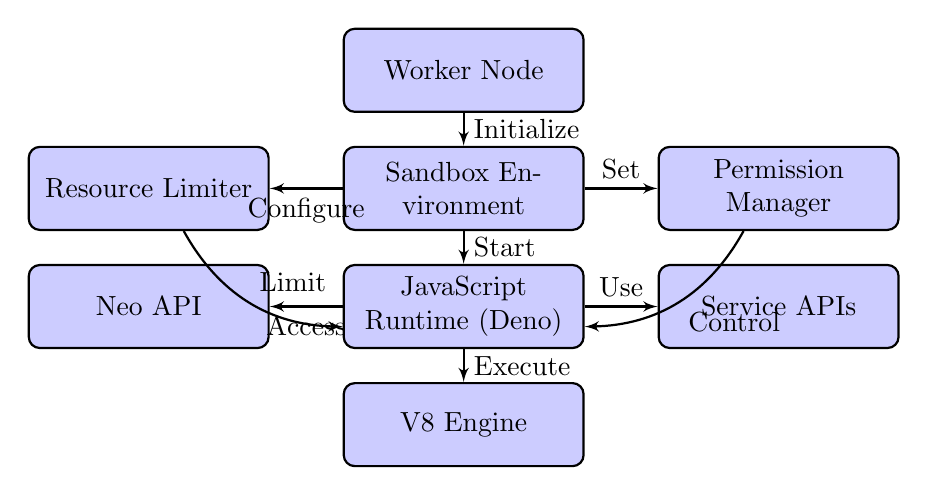
\begin{tikzpicture}[node distance=1.5cm, auto, thick]
    % Define styles
    \tikzstyle{block} = [rectangle, draw, fill=blue!20, text width=8em, text centered, rounded corners, minimum height=3em]
    \tikzstyle{line} = [draw, -latex']
    \tikzstyle{cloud} = [draw, ellipse, fill=red!20, node distance=3cm, minimum height=2em]
    
    % Place nodes
    \node [block] (worker) {Worker Node};
    \node [block, below of=worker] (sandbox) {Sandbox Environment};
    \node [block, below of=sandbox] (runtime) {JavaScript Runtime (Deno)};
    \node [block, left of=sandbox, node distance=4cm] (resource) {Resource Limiter};
    \node [block, right of=sandbox, node distance=4cm] (permission) {Permission Manager};
    \node [block, below of=runtime] (v8) {V8 Engine};
    \node [block, left of=runtime, node distance=4cm] (api) {Neo API};
    \node [block, right of=runtime, node distance=4cm] (services) {Service APIs};
    
    % Draw edges
    \path [line] (worker) -- node {Initialize} (sandbox);
    \path [line] (sandbox) -- node {Configure} (resource);
    \path [line] (sandbox) -- node {Set} (permission);
    \path [line] (sandbox) -- node {Start} (runtime);
    \path [line] (runtime) -- node {Execute} (v8);
    \path [line] (runtime) -- node {Access} (api);
    \path [line] (runtime) -- node {Use} (services);
    \path [line] (resource) to [bend right] node {Limit} (runtime);
    \path [line] (permission) to [bend left] node {Control} (runtime);
    
\end{tikzpicture}
\caption{Sandbox Architecture in Neo Service Layer}
\label{fig:sandbox}
\end{figure}


\begin{definition}[Sandbox]
A Sandbox is a controlled execution environment that restricts the capabilities of the code running within it. Each sandbox has:
\begin{itemize}
    \item Isolation Boundaries: Limits that separate the sandbox from the host system and other sandboxes
    \item Resource Limits: Constraints on CPU, memory, network, and other resources
    \item Permission Model: Rules that determine what APIs and system resources the code can access
    \item Monitoring: Mechanisms for observing and controlling the behavior of the code
\end{itemize}
\end{definition}

\paragraph{Sandbox Architecture}
The Sandbox system implements a multi-layered architecture to provide comprehensive security throughout the function execution lifecycle. At the infrastructure level, the \textbf{Worker Node} serves as the physical or virtual machine that hosts the sandbox environment, providing the foundational hardware and operating system resources. Within each worker, the \textbf{Sandbox Environment} creates an isolated container or virtual machine that provides the first level of isolation, separating function execution from the host system and other functions. For code execution, the \textbf{JavaScript Runtime} based on Deno Core executes the function code with controlled access to system resources, implementing a secure-by-default approach to permissions. To prevent resource abuse, the \textbf{Resource Limiter} continuously monitors and enforces limits on CPU, memory, and other resource usage, ensuring that functions cannot consume excessive resources or interfere with other workloads. Access to external systems is controlled by the \textbf{Permission Manager}, which governs access to APIs, network resources, and other capabilities based on the function's explicitly granted permissions, implementing the principle of least privilege. At the core of the JavaScript execution, the \textbf{V8 Engine} provides the underlying JavaScript engine with additional isolation through its security model, including memory sandboxing and context separation that prevent code from accessing memory outside its designated areas.

\paragraph{Sandbox Security Mechanisms}
The system implements multiple security mechanisms to ensure comprehensive protection throughout the function execution lifecycle. For execution isolation, \textbf{Process Isolation} ensures that functions run in separate processes to prevent interference and limit the impact of crashes, creating strong boundaries between different functions. To control resource access, \textbf{Namespace Isolation} provides each sandbox with its own namespace for files, network, and other resources, preventing access to resources outside the sandbox and creating a contained environment for execution. The system implements \textbf{Capability-Based Security} where functions must explicitly request and be granted permissions for specific capabilities, such as network access or file system operations, enforcing the principle of least privilege at a granular level. To prevent resource monopolization, \textbf{Resource Quotas} impose strict limits on CPU time, memory usage, network bandwidth, and other resources to prevent denial-of-service attacks, ensuring fair resource allocation across all functions. For operational safety, \textbf{Time Limits} enforce maximum execution time limits to prevent infinite loops and resource exhaustion, automatically terminating functions that exceed their allocated time. Network security is maintained through \textbf{Network Filtering} where network access is controlled through fine-grained rules that specify which hosts and ports can be accessed, preventing unauthorized network communication and limiting potential attack vectors.

A formal specification of the sandbox security protocol is provided in Section \ref{subsec:sandbox-protocol}.

\subsection{Sandbox Security Protocol}
\label{subsec:sandbox-protocol}

The Sandbox Security Protocol defines how function execution is isolated and secured to protect both the platform and other functions.

\begin{protocol}[Sandbox Creation and Isolation]
\label{prot:sandbox-creation}
\begin{algorithmic}[1]
\Require Function $F$, Resource limits $L$, Permissions $P$, Worker Node $W$
\Ensure Secure and isolated execution environment

\State \textbf{Resource Allocation:}
\State $\text{resources} \gets W.\text{allocateResources}(L)$

\State \textbf{Container Creation:}
\State $\text{container} \gets W.\text{createContainer}(\text{resources})$
\State $\text{container}.\text{setNamespaces}(\{\text{"pid"}, \text{"net"}, \text{"ipc"}, \text{"mnt"}, \text{"uts"}\})$

\State \textbf{Filesystem Setup:}
\State $\text{rootfs} \gets W.\text{createIsolatedFilesystem}()$
\State $\text{container}.\text{mountFilesystem}(\text{rootfs})$

\State \textbf{Network Configuration:}
\If{$P.\text{allowsNetwork}()$}
    \State $\text{network} \gets W.\text{createNetworkNamespace}(P.\text{networkRules})$
    \State $\text{container}.\text{setNetwork}(\text{network})$
\Else
    \State $\text{container}.\text{disableNetwork}()$
\EndIf

\State \textbf{Resource Limits Setup:}
\State $\text{container}.\text{setCPULimit}(L.\text{cpu})$
\State $\text{container}.\text{setMemoryLimit}(L.\text{memory})$
\State $\text{container}.\text{setDiskIOLimit}(L.\text{diskIO})$
\State $\text{container}.\text{setNetworkIOLimit}(L.\text{networkIO})$

\State \textbf{Runtime Initialization:}
\State $\text{runtime} \gets \text{container}.\text{initializeRuntime}(F.\text{config}.\text{runtime})$
\State $\text{runtime}.\text{setPermissions}(P)$

\State \textbf{Security Policies:}
\State $\text{seccomp} \gets \text{CreateSeccompProfile}(P)$
\State $\text{container}.\text{applySeccompProfile}(\text{seccomp})$
\State $\text{apparmor} \gets \text{CreateAppArmorProfile}(P)$
\State $\text{container}.\text{applyAppArmorProfile}(\text{apparmor})$

\State \textbf{Monitoring Setup:}
\State $\text{monitor} \gets W.\text{createResourceMonitor}(\text{container}, L)$
\State $\text{monitor}.\text{start}()$

\State \Return $\{\text{container}: \text{container}, \text{runtime}: \text{runtime}, \text{monitor}: \text{monitor}\}$
\end{algorithmic}
\end{protocol}

\begin{protocol}[Sandbox Execution Control]
\label{prot:sandbox-execution}
\begin{algorithmic}[1]
\Require Sandbox $S$, Function $F$, Input data $D$, Context $\text{ctx}$, Timeout $T$
\Ensure Secure execution with proper resource control

\State \textbf{Function Loading:}
\State $S.\text{runtime}.\text{loadFunction}(F.\text{code}, F.\text{dependencies})$

\State \textbf{API Access Configuration:}
\For{each $\text{api} \in F.\text{config}.\text{apis}$}
    \If{$F.\text{permissions}.\text{allowsAPI}(\text{api})$}
        \State $S.\text{runtime}.\text{enableAPI}(\text{api})$
    \EndIf
\EndFor

\State \textbf{Execution Timer:}
\State $\text{timer} \gets \text{StartTimer}(T)$

\State \textbf{Execution:}
\State $\text{executionPromise} \gets S.\text{runtime}.\text{executeAsync}(F.\text{entrypoint}, D, \text{ctx})$

\State \textbf{Monitoring Loop:}
\While{$\neg \text{executionPromise}.\text{isResolved}() \land \neg \text{timer}.\text{isExpired}()$}
    \State $\text{metrics} \gets S.\text{monitor}.\text{getMetrics}()$
    \If{$\text{metrics}.\text{exceedsLimits}(F.\text{config}.\text{limits})$}
        \State $S.\text{runtime}.\text{terminate}()$
        \State \Return $\{\text{error}: \text{"Resource limits exceeded"}, \text{metrics}: \text{metrics}\}$
    \EndIf
    \State $\text{Sleep}(10\text{ ms})$
\EndWhile

\If{$\text{timer}.\text{isExpired}()$}
    \State $S.\text{runtime}.\text{terminate}()$
    \State \Return $\{\text{error}: \text{"Execution timeout"}, \text{timeout}: T\}$
\EndIf

\State \textbf{Result Capture:}
\State $\text{result} \gets \text{executionPromise}.\text{getResult}()$

\State \textbf{Cleanup:}
\State $S.\text{runtime}.\text{cleanup}()$
\State $S.\text{monitor}.\text{stop}()$

\State \Return $\text{result}$
\end{algorithmic}
\end{protocol}


\paragraph{JavaScript Runtime Security}
The Deno Core JavaScript runtime provides additional security features that enhance the overall sandbox protection model. The runtime implements a \textbf{Secure Module System} where modules must be explicitly imported and can only access the capabilities they are granted, preventing unauthorized code execution and limiting the potential attack surface. For improved code quality and security, \textbf{TypeScript Support} provides static type checking that can catch potential security issues at compile time, reducing the risk of type-related vulnerabilities and improving code reliability. Access to potentially dangerous functionality is controlled through \textbf{Controlled API Access} where access to sensitive APIs is managed through a permission system that requires explicit grants, ensuring that functions can only use the specific capabilities they need. The system follows \textbf{Secure Defaults} principles where, by default, functions have no access to the file system, network, or environment variables, requiring explicit permission for each capability, implementing a zero-trust security model that minimizes the risk of unauthorized access.

\subsubsection{Trusted Execution Environment (TEE)}
\label{subsubsec:tee}

The Trusted Execution Environment (TEE) service provides a secure and isolated environment for executing sensitive computations off-chain. This service is particularly valuable for applications that require privacy, high computational resources, or access to sensitive data that cannot be exposed on the public blockchain.

% This file should only be \input{} in a document that loads the tikz package
% Do not compile this file directly with pdflatex

\begin{figure}[ht]
\centering
\begin{tikzpicture}[
    box/.style={rectangle, draw, rounded corners, fill=white, 
               minimum width=2.5cm, minimum height=1.2cm, text centered},
    line/.style={-latex, thick}
]
    % Nodes - Increased vertical spacing and better alignment
    \node[box, fill=blue!10] (app) at (0,8) {Application};
    \node[box, fill=green!10] (enclave) at (0,4) {Trusted Enclave};
    \node[box, fill=red!10] (blockchain) at (0,0) {Blockchain};
    
    % Components inside TEE - Increased horizontal spacing and size
    \node[box, fill=yellow!10, minimum width=2cm, minimum height=1cm] (processor) 
         at (-5,4) {Secure Processor};
    \node[box, fill=yellow!10, minimum width=2cm, minimum height=1cm] (memory) 
         at (5,4) {Encrypted Memory};
         
    % Draw a box around TEE components - Further enlarged and styled
    \draw[dashed, thick, rounded corners=5pt] (-6.5,2) rectangle (6.5,6);
    
    % Label for the TEE box
    \node[font=\small\bfseries] at (0,5.7) {Trusted Execution Environment};
    
    % Data flow connections with clear labels
    \draw[line] (app) -- node[above-arrow-text, right, pos=0.3] {Encrypted Data} (enclave);
    \draw[line] (enclave) -- node[above-arrow-text, right, pos=0.7] {Verified Results} (blockchain);
    \draw[line] (processor) -- node[above-arrow-text, pos=0.5] {Secure Operations} (memory);
    
    % Additional note - Adjusted position and styled for clarity
    \draw[->, thick] (7.5,5) -- (6.8,5);
    \draw[->, thick] (7.5,3) -- (6.8,3);
    \node[above-arrow-text, align=center, text width=3cm] at (9,4) {\textbf{Hardware Protection \& Isolation}};
\end{tikzpicture}
\caption{Trusted Execution Environment Service}
\label{fig:tee-service}
\end{figure}


\begin{definition}[Trusted Execution Environment]
A Trusted Execution Environment is a secure area within a processor that ensures the confidentiality and integrity of code and data loaded inside it. TEEs provide hardware-level isolation, protecting sensitive operations from the host operating system and other applications.
\end{definition}

The TEE service supports multiple platforms and security levels to accommodate diverse hardware environments and security requirements. The service provides support for \textbf{Intel SGX}, which offers secure enclaves within Intel processors that create isolated memory regions protected from the rest of the system, including privileged software. For AMD-based systems, \textbf{AMD SEV} (Secure Encrypted Virtualization) is supported, providing memory encryption for virtual machines to protect against physical memory attacks and hypervisor vulnerabilities. Mobile and embedded applications can leverage \textbf{ARM TrustZone}, a secure execution environment for ARM processors that creates a hardware-separated secure world for sensitive operations. For cloud deployments, the service integrates with \textbf{Cloud TEEs}, which are confidential computing offerings from major cloud providers that enable secure processing in shared cloud environments while maintaining data confidentiality.

Applications can leverage the TEE service for various use cases that require enhanced security and privacy guarantees. For sensitive data processing, \textbf{Private Computation} enables applications to process sensitive data without revealing it to the blockchain, maintaining confidentiality while still allowing verification of computation results. In scenarios involving multiple stakeholders, \textbf{Secure Multi-Party Computation} facilitates collaborative computation between mutually distrusting parties, allowing them to jointly compute results without revealing their individual inputs to each other. For blockchain applications requiring privacy, \textbf{Confidential Smart Contracts} enable the execution of contracts with private state and logic, keeping sensitive business logic and transaction details confidential while still leveraging blockchain security. Critical security operations benefit from \textbf{Secure Key Management} capabilities, providing robust protection of cryptographic keys and credentials against both software and hardware attacks, ensuring that even if the host system is compromised, the keys remain secure.

The TEE service provides attestation reports that verify the integrity and authenticity of the execution environment. These reports can be verified on-chain, allowing smart contracts to trust the results of off-chain computations.

\paragraph{TEE Execution Protocol}
The TEE service implements a comprehensive protocol for secure execution that ensures confidentiality and integrity throughout the computation lifecycle. The process begins with \textbf{Code Submission}, where the application submits the code to be executed in the TEE, along with any required input data, initiating the secure computation process. Based on the application's requirements, \textbf{Environment Selection} occurs, where the service selects an appropriate TEE environment based on the security requirements, availability, and capabilities, ensuring optimal execution conditions. The selected environment then undergoes \textbf{Enclave Initialization}, where the TEE initializes a secure enclave, loading the code and preparing the execution environment with the necessary resources and security configurations. To establish trust, \textbf{Remote Attestation} generates an attestation report that proves the authenticity and integrity of the enclave to the application, providing cryptographic evidence that the code is running in a genuine and unmodified TEE. Before execution, \textbf{Secure Input Processing} ensures that input data is securely transferred to the enclave, often using encryption to protect sensitive information during transit, preventing exposure of confidential inputs. The core computation occurs during \textbf{Protected Execution}, where the code executes within the enclave with hardware-level protection against external observation or interference, ensuring that even privileged software cannot access the computation. After execution, \textbf{Result Sealing} cryptographically protects the execution results to ensure they can only be accessed by authorized parties, maintaining confidentiality beyond the execution phase. The protected results undergo \textbf{Secure Output Delivery}, where the sealed results are securely delivered to the requesting application or stored for later retrieval, ensuring end-to-end protection of sensitive outputs. Finally, \textbf{Verification} allows the application to verify the authenticity of the results using the attestation report and cryptographic proofs, establishing a chain of trust from execution to result consumption.

\paragraph{TEE Integration with Blockchain}
The TEE service provides specialized integration with blockchain networks, creating a powerful bridge between on-chain security and off-chain confidentiality. Through \textbf{On-Chain Verification}, smart contracts can verify TEE attestation reports directly on the blockchain, enabling trust in off-chain computation results and creating a verifiable link between private computations and public consensus. For applications requiring data privacy, \textbf{Confidential State} capabilities allow TEEs to maintain confidential state that is not visible on the public blockchain but can be used in computations, enabling applications to leverage blockchain security without sacrificing data confidentiality. To enhance transaction privacy, \textbf{Private Transactions} processing allows TEEs to handle private transaction data off-chain while publishing only necessary verification information on-chain, striking a balance between privacy and verifiability. For external data integration, \textbf{Secure Oracles} functionality enables TEEs to serve as secure oracles that access external data sources while providing cryptographic guarantees of data integrity, creating a trusted channel for bringing real-world data onto the blockchain with strong security assurances.

\subsubsection{Smart Contract Integration}
\label{subsubsec:smart-contract}

The Neo Service Layer provides comprehensive support for smart contract development, deployment, and integration. This system enables developers to create powerful decentralized applications that leverage both on-chain security and off-chain capabilities.

\begin{figure}[h]
\centering
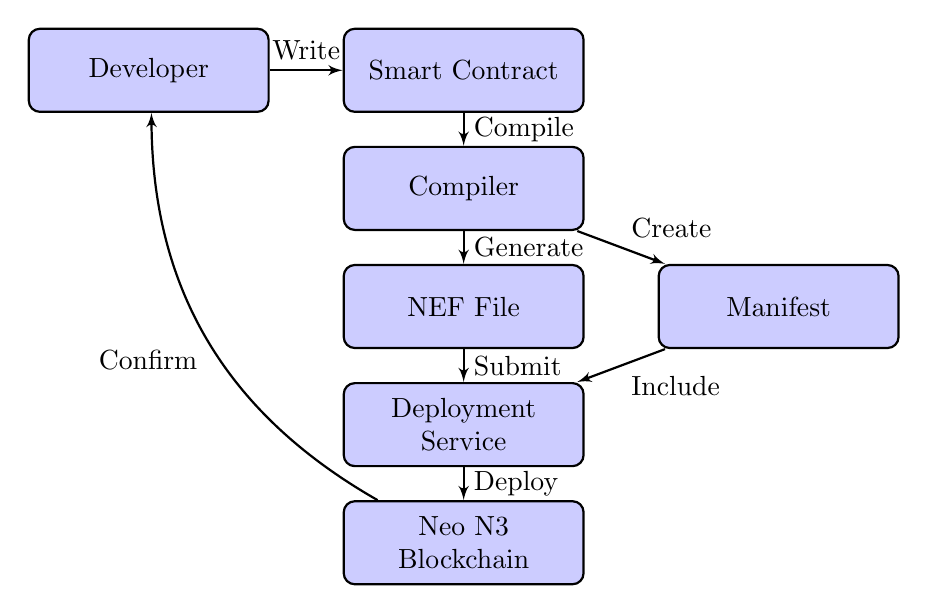
\begin{tikzpicture}[node distance=1.5cm, auto, thick]
    % Define styles
    \tikzstyle{block} = [rectangle, draw, fill=blue!20, text width=8em, text centered, rounded corners, minimum height=3em]
    \tikzstyle{line} = [draw, -latex']
    \tikzstyle{cloud} = [draw, ellipse, fill=red!20, node distance=3cm, minimum height=2em]
    
    % Place nodes
    \node [block] (developer) {Developer};
    \node [block, right of=developer, node distance=4cm] (contract) {Smart Contract};
    \node [block, below of=contract] (compiler) {Compiler};
    \node [block, below of=compiler] (nef) {NEF File};
    \node [block, right of=nef, node distance=4cm] (manifest) {Manifest};
    \node [block, below of=nef] (deploy) {Deployment Service};
    \node [block, below of=deploy] (blockchain) {Neo N3 Blockchain};
    
    % Draw edges
    \path [line] (developer) -- node {Write} (contract);
    \path [line] (contract) -- node {Compile} (compiler);
    \path [line] (compiler) -- node {Generate} (nef);
    \path [line] (compiler) -- node {Create} (manifest);
    \path [line] (nef) -- node {Submit} (deploy);
    \path [line] (manifest) -- node {Include} (deploy);
    \path [line] (deploy) -- node {Deploy} (blockchain);
    \path [line] (blockchain) to [bend left] node {Confirm} (developer);
    
\end{tikzpicture}
\caption{Smart Contract Deployment in Neo Service Layer}
\label{fig:smart-contract}
\end{figure}


\begin{definition}[Smart Contract Integration]
Smart Contract Integration refers to the seamless connection between blockchain-based smart contracts and the Neo Service Layer components. This integration enables contracts to access off-chain services while maintaining security and decentralization.
\end{definition}

\paragraph{Smart Contract Development}
The Neo Service Layer provides tools and libraries that simplify smart contract development, enabling developers to create sophisticated blockchain applications with minimal friction. Developers can leverage \textbf{Contract Templates}, which are pre-built templates for common contract patterns that integrate with Service Layer components, accelerating development by providing proven, secure implementations of frequently used functionality. To facilitate integration, \textbf{Service Layer SDKs} offer language-specific libraries that enable seamless interaction between smart contracts and Service Layer services, providing type-safe interfaces and abstractions that hide the complexity of the underlying protocols. For quality assurance, a comprehensive \textbf{Testing Framework} provides specialized tools for simulating contract interactions with Service Layer components, allowing developers to verify functionality and security before deployment to production environments. The development experience is enhanced through an \textbf{Development Environment} with integrated debugging capabilities specifically designed for contracts that use Service Layer features, enabling developers to efficiently identify and resolve issues throughout the development lifecycle.

\paragraph{Smart Contract Deployment Process}
The deployment process for smart contracts involves several interconnected steps that ensure proper integration with the Neo ecosystem. The process begins with \textbf{Contract Development}, where developers write smart contracts using Neo's supported languages (C\#, Python, Go, TypeScript) with Service Layer integration, leveraging the specialized libraries and SDKs to create contracts that can interact with off-chain services. Once the contract code is complete, \textbf{Compilation} transforms the high-level code into Neo Executable Format (NEF) files, which contain the bytecode that runs on the Neo Virtual Machine (NeoVM), optimizing the code for on-chain execution. To define the contract's capabilities and interfaces, \textbf{Manifest Creation} generates a manifest file that describes the contract's interface, permissions, and other metadata, establishing the contract's identity and access rights within the blockchain ecosystem. For contracts that leverage Service Layer functionality, \textbf{Service Registration} connects them with the relevant services to establish the necessary connections, enabling seamless interaction between on-chain and off-chain components. The actual blockchain integration occurs during \textbf{Deployment}, where the NEF file and manifest are deployed to the Neo N3 blockchain through a transaction, making the contract available for interaction on the network. After deployment, \textbf{Verification} ensures that the deployed contract matches the source code and functions as expected, confirming that no errors occurred during the compilation and deployment process. Finally, \textbf{Integration Configuration} sets up Service Layer components to interact with the deployed contract, establishing event listeners, callbacks, and other integration points that enable the contract to leverage the full capabilities of the Neo Service Layer.

A formal specification of the Smart Contract Integration protocol is provided in Section \ref{subsec:smart-contract-protocol}.

\subsection{Smart Contract Integration Protocol}
\label{subsec:smart-contract-protocol}

The Smart Contract Integration Protocol defines how smart contracts are deployed and integrated with the Neo Service Layer.

\begin{protocol}[Smart Contract Deployment]
\label{prot:smart-contract-deployment}
\begin{algorithmic}[1]
\Require Contract source code $C$, Developer $D$, Compiler $\text{comp}$, Blockchain $B$
\Ensure Contract is properly deployed and registered with Service Layer

\State \textbf{Contract Compilation:}
\State $\text{nef} \gets \text{comp}.\text{compile}(C)$
\State $\text{manifest} \gets \text{comp}.\text{generateManifest}(C)$

\State \textbf{Contract Validation:}
\State $\text{valid} \gets \text{ValidateContract}(\text{nef}, \text{manifest})$
\If{$\neg \text{valid}$}
    \State \Return $\{\text{error}: \text{"Invalid contract"}\}$
\EndIf

\State \textbf{Service Layer Integration:}
\For{each $\text{service} \in \text{manifest}.\text{services}$}
    \State $\text{ServiceRegistry}.\text{registerContractService}(\text{service}.\text{name}, \text{service}.\text{config})$
\EndFor

\State \textbf{Deployment Transaction:}
\State $\text{tx} \gets B.\text{createDeployTransaction}(\text{nef}, \text{manifest}, D.\text{address})$
\State $\text{signedTx} \gets D.\text{signTransaction}(\text{tx})$

\State \textbf{Transaction Submission:}
\State $\text{txHash} \gets B.\text{submitTransaction}(\text{signedTx})$

\State \textbf{Transaction Monitoring:}
\State $\text{confirmed} \gets \text{false}$
\While{$\neg \text{confirmed}$}
    \State $\text{receipt} \gets B.\text{getTransactionReceipt}(\text{txHash})$
    \If{$\text{receipt} \neq \text{null}$}
        \State $\text{confirmed} \gets \text{true}$
        \If{$\text{receipt}.\text{status} = \text{"success"}$}
            \State $\text{contractHash} \gets \text{receipt}.\text{contractHash}$
        \Else
            \State \Return $\{\text{error}: \text{"Deployment failed"}, \text{receipt}: \text{receipt}\}$
        \EndIf
    \EndIf
    \If{$\neg \text{confirmed}$}
        \State $\text{Sleep}(1\text{ second})$
    \EndIf
\EndWhile

\State \textbf{Service Layer Registration:}
\State $\text{ContractRegistry}.\text{registerContract}(\text{contractHash}, \text{manifest}, \text{nef})$

\State \textbf{Event Listener Setup:}
\For{each $\text{event} \in \text{manifest}.\text{events}$}
    \State $\text{EventSystem}.\text{registerEventListener}(\text{contractHash}, \text{event}.\text{name})$
\EndFor

\State \Return $\{\text{success}: \text{true}, \text{contractHash}: \text{contractHash}, \text{txHash}: \text{txHash}\}$
\end{algorithmic}
\end{protocol}

\begin{protocol}[Service Layer Contract Integration]
\label{prot:service-layer-integration}
\begin{algorithmic}[1]
\Require Contract hash $H$, Service type $T$, Integration configuration $I$, Service Layer $S$
\Ensure Contract is properly integrated with the specified Service Layer component

\State \textbf{Contract Verification:}
\State $\text{contract} \gets \text{ContractRegistry}.\text{getContract}(H)$
\If{$\text{contract} = \text{null}$}
    \State \Return $\{\text{error}: \text{"Contract not found"}\}$
\EndIf

\State \textbf{Service Verification:}
\State $\text{service} \gets S.\text{getService}(T)$
\If{$\text{service} = \text{null}$}
    \State \Return $\{\text{error}: \text{"Service not found"}\}$
\EndIf

\State \textbf{Permission Check:}
\State $\text{hasPermission} \gets \text{contract}.\text{manifest}.\text{permissions}.\text{hasPermission}(T)$
\If{$\neg \text{hasPermission}$}
    \State \Return $\{\text{error}: \text{"Contract does not have permission for this service"}\}$
\EndIf

\State \textbf{Integration Configuration:}
\State $\text{config} \gets \text{service}.\text{createIntegrationConfig}(H, I)$

\State \textbf{Integration Type-Specific Setup:}
\If{$T = \text{"GasBank"}$}
    \State $\text{account} \gets \text{service}.\text{createAccount}(H, I.\text{feeModel})$
    \State $\text{config}.\text{accountAddress} \gets \text{account}.\text{address}$
\ElsIf{$T = \text{"MetaTransaction"}$}
    \State $\text{service}.\text{registerContractForRelaying}(H, I.\text{methods})$
\ElsIf{$T = \text{"Oracle"}$}
    \State $\text{service}.\text{registerCallbackContract}(H, I.\text{callbackMethod})$
\ElsIf{$T = \text{"TEE"}$}
    \State $\text{service}.\text{registerAttestationVerifier}(H, I.\text{verifierMethod})$
\EndIf

\State \textbf{Event Listener Setup:}
\For{each $\text{event} \in I.\text{events}$}
    \State $\text{EventSystem}.\text{registerServiceEventHandler}(T, H, \text{event}.\text{name}, \text{event}.\text{handler})$
\EndFor

\State \textbf{Integration Storage:}
\State $\text{IntegrationRegistry}.\text{storeIntegration}(H, T, \text{config})$

\State \Return $\{\text{success}: \text{true}, \text{contract}: H, \text{service}: T, \text{config}: \text{config}\}$
\end{algorithmic}
\end{protocol}


\paragraph{Service Layer Integration Patterns}
Smart contracts can integrate with the Service Layer through several patterns that enable powerful combinations of on-chain and off-chain capabilities. Through \textbf{Event-Driven Integration}, contracts emit events that trigger Service Layer functions, enabling off-chain processing of on-chain actions and creating responsive systems that can react to blockchain state changes with complex off-chain logic. For accessing external data, \textbf{Oracle Integration} allows contracts to request information from the Oracle Service, enabling access to real-world information not natively available on the blockchain such as price feeds, weather data, or sports results. To improve user experience, \textbf{Gas Bank Integration} enables contracts to interact with the Gas Bank service to implement gas-free transactions for users, removing the friction of requiring users to hold cryptocurrency for transaction fees. Similarly, \textbf{Meta Transaction Integration} allows contracts to support meta transactions, enabling users to interact with blockchain applications without directly paying for transaction fees, with costs covered by application developers or subsidized through other mechanisms. For privacy-sensitive operations, \textbf{TEE Integration} allows contracts to delegate sensitive computations to the Trusted Execution Environment service, enabling private processing with on-chain verification that maintains confidentiality while leveraging blockchain security. Advanced user experiences are enabled through \textbf{Abstract Account Integration}, where contracts interact with the Abstract Account service to support sophisticated account management features such as social recovery, multi-signature control, and programmable authorization policies.

\paragraph{Smart Contract Security}
The Neo Service Layer enhances smart contract security through several mechanisms that work together to create a comprehensive security framework. For mathematical assurance of correctness, \textbf{Formal Verification} tools enable developers to formally verify contract behavior and security properties, providing mathematical proofs that contracts behave as intended under all possible conditions. To identify potential vulnerabilities early in the development process, \textbf{Security Scanning} provides automated analysis for common vulnerabilities and security issues, detecting patterns that could lead to exploits or unintended behavior before deployment. Developers are guided by \textbf{Secure Development Guidelines} that provide best practices and patterns for developing secure contracts that integrate with Service Layer components, establishing a foundation of security knowledge that helps prevent common mistakes. For thorough security assessment, \textbf{Auditing Tools} offer specialized capabilities for auditing contracts that use Service Layer features, enabling security professionals to comprehensively evaluate contract security with awareness of Service Layer integration points. After deployment, \textbf{Monitoring and Alerting} provides real-time monitoring of contract behavior with alerts for suspicious activities, enabling rapid response to potential security incidents and unusual patterns that might indicate an attack in progress.

\subsubsection{Advanced Cryptographic Services}
\label{subsubsec:advanced-crypto}

The Neo Service Layer includes advanced cryptographic services that provide cutting-edge privacy, security, and computational capabilities. These services enable applications to leverage sophisticated cryptographic techniques without requiring deep expertise in cryptography.

\begin{figure}[h]
\centering
\begin{tikzpicture}[node distance=1.5cm, auto, thick]
    % Define styles
    \tikzset{
        block/.style = [rectangle, draw, fill=blue!20, text width=8em, text centered, rounded corners, minimum height=3em],
        line/.style = [draw, -latex', thick],
        cloud/.style = [draw, ellipse, fill=red!20, minimum height=2em]
    }
    
    % Place nodes
    \node [block] (service) {Neo Service Layer};
    
    \node [block, below of=service, node distance=3cm, xshift=-6cm] (tee) {Trusted Execution Environment};
    \node [block, below of=tee, xshift=-2cm] (sgx) {Intel SGX};
    \node [block, below of=tee, xshift=2cm] (nitro) {AWS Nitro};
    
    \node [block, below of=service, node distance=3cm] (fhe) {Fully Homomorphic Encryption};
    \node [block, below of=fhe, xshift=-2cm] (tfhe) {TFHE};
    \node [block, below of=fhe, xshift=2cm] (openfhe) {OpenFHE};
    
    \node [block, below of=service, node distance=3cm, xshift=6cm] (zk) {Zero-Knowledge Computing};
    \node [block, below of=zk, xshift=-2cm] (zokrates) {ZoKrates};
    \node [block, below of=zk, xshift=2cm] (bulletproofs) {Bulletproofs};
    
    % Draw edges
    \path [line] (service) -- (tee);
    \path [line] (service) -- (fhe);
    \path [line] (service) -- (zk);
    
    \path [line] (tee) -- (sgx);
    \path [line] (tee) -- (nitro);
    
    \path [line] (fhe) -- (tfhe);
    \path [line] (fhe) -- (openfhe);
    
    \path [line] (zk) -- (zokrates);
    \path [line] (zk) -- (bulletproofs);
    
\end{tikzpicture}
\caption{Advanced Cryptographic Services in Neo Service Layer}
\label{fig:advanced-crypto}
\end{figure}


\begin{definition}[Advanced Cryptographic Service]
An Advanced Cryptographic Service is a specialized component that implements sophisticated cryptographic protocols to enable secure computation, privacy-preserving operations, or enhanced security features beyond what is available in standard blockchain environments.
\end{definition}

The Neo Service Layer provides three main categories of advanced cryptographic services that enable sophisticated privacy and security capabilities. \textbf{Trusted Execution Environment (TEE)} technology offers hardware-based secure enclaves for confidential computation, creating isolated execution environments protected by the processor itself to ensure that even privileged software cannot access sensitive data or code. For computations on sensitive data, \textbf{Fully Homomorphic Encryption (FHE)} enables computation on encrypted data without requiring decryption, allowing operations to be performed while maintaining data confidentiality throughout the entire processing lifecycle. To prove statements without revealing underlying information, \textbf{Zero-Knowledge Computing (ZK)} facilitates the generation and verification of proofs that demonstrate knowledge without exposing the underlying information, enabling privacy-preserving verification of claims, computations, and identities.

\paragraph{Fully Homomorphic Encryption Service}
The FHE service enables computation on encrypted data without requiring decryption, providing powerful privacy-preserving capabilities for sensitive applications. The service supports multiple \textbf{Encryption Schemes}, including TFHE, BFV, and CKKS, each optimized for different types of operations, allowing developers to select the most appropriate scheme for their specific use case requirements. For computational flexibility, the service provides various \textbf{Operation Types} on encrypted data, including arithmetic operations, boolean operations, and approximate operations on real numbers, enabling a wide range of privacy-preserving computations from simple calculations to complex algorithms. Secure \textbf{Key Management} is a core component of the service, providing secure generation, storage, and distribution of encryption keys, including support for threshold key generation and multi-party computation, ensuring that encryption keys remain protected throughout their lifecycle. To address the computational intensity of FHE, the service implements \textbf{Performance Optimization} techniques for enhancing FHE performance, including batching, parallelization, and hardware acceleration, making privacy-preserving computation practical for real-world applications. For blockchain applications, the service offers \textbf{Integration Patterns} for combining FHE with blockchain systems, including on-chain verification of off-chain FHE computations, enabling applications to leverage both the privacy benefits of FHE and the security guarantees of blockchain technology.

\paragraph{Zero-Knowledge Computing Service}
The ZK service enables the generation and verification of zero-knowledge proofs, providing powerful privacy-preserving capabilities for blockchain applications. The service supports multiple \textbf{Proof Systems}, including SNARKs, STARKs, and Bulletproofs, each with different trade-offs in terms of setup requirements, proof size, and verification time, allowing developers to select the most appropriate system for their specific requirements. For developer accessibility, \textbf{Circuit Compilation} tools facilitate the conversion of high-level program descriptions into arithmetic circuits suitable for zero-knowledge proofs, abstracting away the complex mathematical details and enabling developers to focus on application logic. The core functionality includes \textbf{Proof Generation} capabilities for efficiently creating proofs that demonstrate the correctness of computations without revealing inputs or intermediate values, maintaining privacy while ensuring verifiability. For blockchain integration, \textbf{On-Chain Verification} provides seamless integration with Neo N3 smart contracts for on-chain verification of zero-knowledge proofs, enabling trustless verification of private computations. The service supports various \textbf{Privacy-Preserving Applications} with pre-built patterns for common privacy-preserving use cases, such as confidential transactions, private voting, and anonymous credentials, accelerating the development of privacy-focused blockchain applications.

\paragraph{Cross-Service Integration}
The advanced cryptographic services can be combined to create powerful hybrid solutions that leverage the complementary strengths of different cryptographic approaches. The \textbf{TEE-FHE Hybrid} integration uses Trusted Execution Environments to accelerate Fully Homomorphic Encryption operations while providing additional security guarantees, addressing the performance limitations of FHE while enhancing its security properties through hardware protection. For privacy-preserving proof generation, the \textbf{TEE-ZK Hybrid} approach uses TEEs to generate zero-knowledge proofs more efficiently while ensuring the privacy of the witness data, significantly improving the performance of complex zero-knowledge proof generation while maintaining strong privacy guarantees. To verify encrypted computations, the \textbf{FHE-ZK Hybrid} combines zero-knowledge proofs to verify the correctness of FHE computations without revealing the encryption keys or the computation itself, creating a verifiable yet private computational framework. For collaborative applications, \textbf{Multi-Party Computation} integrations combine multiple cryptographic techniques to enable secure computation among mutually distrusting parties, allowing organizations to jointly compute results without revealing their sensitive inputs to each other.

A formal specification of the Advanced Cryptographic Services protocol is provided in Section \ref{subsec:advanced-crypto-protocol}.

% This file should only be \input{} in a document that loads the algorithm and algorithmic packages
% Do not compile this file directly with pdflatex

\begin{algorithm}
\caption{Advanced Cryptography Protocol}
\label{alg:advanced-crypto}
\begin{algorithmic}[1]
\Require Cryptographic operation, input data, security parameters
\Ensure Secure execution of complex cryptographic operations

\State \textbf{Initialize:} Validate operation request
\State $request \gets \{operation, inputData, securityParams\}$
\If {$!isSupportedOperation(request.operation)$}
    \State \Return Unsupported operation error
\EndIf

\State \textbf{Verify:} Check input data and parameters
\If {$!isValidInput(request.inputData, request.operation)$}
    \State \Return Invalid input data error
\EndIf
\If {$!securityParamsValid(request.securityParams, request.operation)$}
    \State \Return Invalid security parameters error
\EndIf

\State \textbf{Prepare:} Set up cryptographic context
\State $context \gets createCryptoContext(request.operation, request.securityParams)$
\State $sanitizedInput \gets sanitizeInput(request.inputData)$

\State \textbf{Execute:} Perform the cryptographic operation
\If {$request.operation == "ZKP\_GENERATE"$}
    \State $result \gets generateZeroKnowledgeProof(sanitizedInput, context)$
\ElsIf {$request.operation == "ZKP\_VERIFY"$}
    \State $result \gets verifyZeroKnowledgeProof(sanitizedInput, context)$
\ElsIf {$request.operation == "MPC\_COMPUTE"$}
    \State $result \gets secureMultiPartyComputation(sanitizedInput, context)$
\ElsIf {$request.operation == "FHE\_ENCRYPT"$}
    \State $result \gets fullyHomomorphicEncrypt(sanitizedInput, context)$
\ElsIf {$request.operation == "FHE\_COMPUTE"$}
    \State $result \gets fullyHomomorphicCompute(sanitizedInput, context)$
\ElsIf {$request.operation == "FHE\_DECRYPT"$}
    \State $result \gets fullyHomomorphicDecrypt(sanitizedInput, context)$
\EndIf

\State \textbf{Validate:} Verify result integrity
\If {$!isValidResult(result, request.operation)$}
    \State $logOperationFailure(request, "Invalid result")$
    \State \Return Operation failed, invalid result
\EndIf

\State \textbf{Secure:} Apply additional security measures
\State $securedResult \gets applySecurityWrappers(result, request.securityParams)$
\State $logOperationSuccess(request.operation, request.securityParams)$

\State \Return Success, securedResult
\end{algorithmic}
\end{algorithm} 

\paragraph{Application Domains}
The advanced cryptographic services enable a wide range of privacy-preserving and secure applications across diverse domains. In the financial sector, \textbf{Private DeFi} applications preserve user privacy while ensuring compliance with regulations, enabling financial transactions that protect sensitive information while still meeting regulatory requirements. For identity management, \textbf{Confidential Identity} systems allow selective disclosure of attributes without revealing unnecessary information, giving users control over their personal data while still providing necessary verification to service providers. In data analytics, \textbf{Secure Multi-Party Analytics} enables collaborative analysis on sensitive data without exposing the raw data to any party, allowing organizations to derive insights from combined datasets without compromising data confidentiality. For organizational decision-making, \textbf{Private Governance} systems protect voter privacy while ensuring correct tallying, enabling transparent yet private voting processes for corporate governance, DAOs, and other collective decision-making contexts. In logistics and manufacturing, \textbf{Confidential Supply Chain} tracking preserves commercial confidentiality while enabling verification of claims, allowing businesses to validate supply chain information without exposing proprietary details about suppliers, pricing, or volumes.

\subsubsection{Abstract Account Service}
\label{subsubsec:abstract-account}

The Abstract Account service provides advanced account management capabilities beyond what is possible with standard blockchain accounts. This service enables features such as multi-signature control, account recovery, and programmable authorization policies, creating a flexible foundation for sophisticated account management.

\begin{figure}[h]
\centering
\begin{tcolorbox}[
    enhanced,
    colback=blue!5!white,
    colframe=blue!75!black,
    arc=5mm,
    boxrule=1.5pt,
    title=Abstract Account Architecture,
    fonttitle=\bfseries,
    coltitle=white,
    attach boxed title to top left={yshift=-2mm, xshift=5mm},
    boxed title style={colback=blue!75!black, rounded corners},
    shadow={2mm}{-2mm}{0mm}{black!50},
    drop fuzzy shadow
]
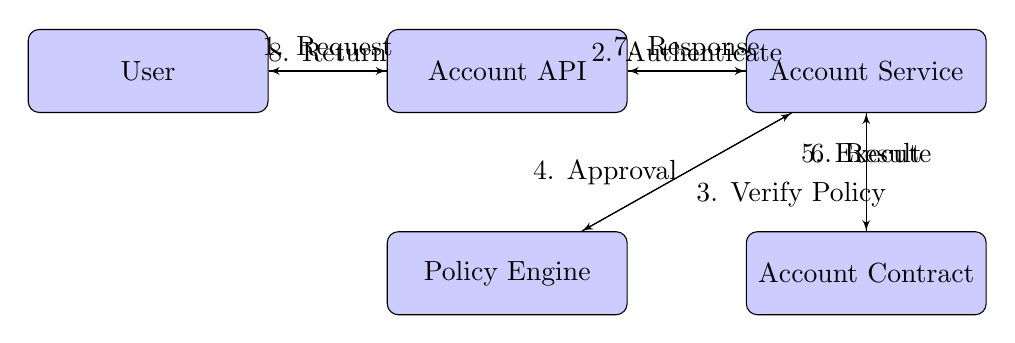
\begin{tikzpicture}[node distance=1.5cm, auto]
    % Define styles
    \tikzstyle{block} = [rectangle, draw, fill=blue!20, text width=8em, text centered, rounded corners, minimum height=3em]
    \tikzstyle{line} = [draw, -latex']
    \tikzstyle{cloud} = [draw, ellipse, fill=red!20, node distance=3cm, minimum height=2em]
    
    % Place nodes
    \node [block] (user) {User};
    \node [block, right=of user] (api) {Account API};
    \node [block, right=of api] (service) {Account Service};
    \node [block, below=of service] (contract) {Account Contract};
    \node [block, below=of api] (policy) {Policy Engine};
    
    % Draw edges
    \path [line] (user) -- node {1. Request} (api);
    \path [line] (api) -- node {2. Authenticate} (service);
    \path [line] (service) -- node {3. Verify Policy} (policy);
    \path [line] (policy) -- node [left] {4. Approval} (service);
    \path [line] (service) -- node [above] {5. Execute} (contract);
    \path [line] (contract) -- node [above] {6. Result} (service);
    \path [line] (service) -- node [above] {7. Response} (api);
    \path [line] (api) -- node [above] {8. Return} (user);
\end{tikzpicture}
\end{tcolorbox}
\caption{Abstract Account Architecture and Flow}
\label{fig:abstract-account}
\end{figure}


\begin{definition}[Abstract Account]
An Abstract Account is a smart contract-based account that implements advanced control and authorization mechanisms. Each abstract account has a unique Address that serves as its identifier in the blockchain ecosystem, an Owner who acts as the primary controller of the account, Controllers who are additional entities authorized to perform operations on the account, a Policy that defines the rules governing how operations are authorized, and a Contract that implements the underlying smart contract logic for the account.
\end{definition}

The Abstract Account service supports various account operations that enable flexible and secure account management. Users can modify account access by \textbf{Adding/Removing Controllers}, which allows adjusting the set of entities that can control the account, enabling dynamic access management as organizational needs change. Security policies can be adapted through \textbf{Updating Policies}, which allows changing the rules for operation authorization, such as modifying signature thresholds or adding time-based restrictions. For protection against key loss, \textbf{Account Recovery} mechanisms enable recovering access to an account after key loss through predefined recovery procedures like social recovery or backup key activation. Beyond standard operations, \textbf{Custom Operations} support application-specific functions defined by the account contract, allowing developers to extend account functionality for specific use cases such as scheduled transactions or conditional approvals.

This service is particularly valuable for applications requiring enhanced security, corporate governance, or complex authorization workflows. By abstracting account management into a dedicated service, applications can implement sophisticated control mechanisms without burdening users with technical complexity.

\subsection{Integration with Neo Ecosystem}
\label{subsec:nsl-integration}

The Neo Service Layer is designed to integrate seamlessly with the broader Neo ecosystem, enhancing the capabilities of existing components and enabling new synergies between different parts of the platform.

\begin{figure}[htbp]
\centering
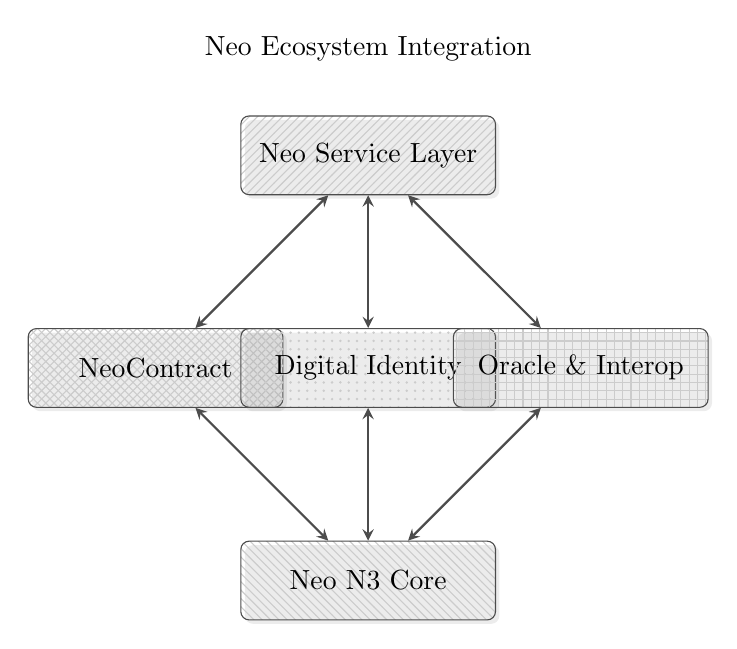
\begin{tikzpicture}[
    scale=0.9,
    box/.style={rectangle, draw=black!70, rounded corners=3pt, 
               fill=white, text width=3cm, align=center, minimum height=1cm,
               pattern=#1, pattern color=black!20,
               drop shadow={opacity=0.15, shadow xshift=0.5mm, shadow yshift=-0.5mm}},
    arrow/.style={->, >=stealth, thick, draw=black!70},
    dashed_arrow/.style={->, >=stealth, thick, dashed, draw=black!70},
    bidirectional/.style={<->, >=stealth, thick, draw=black!70}
]

% Neo Ecosystem Components
\node[box=north east lines] (nsl) at (0,3) {Neo Service Layer};
\node[box=crosshatch] (contract) at (-3,0) {NeoContract};
\node[box=dots] (identity) at (0,0) {Digital Identity};
\node[box=grid] (oracle) at (3,0) {Oracle \& Interop};
\node[box=north west lines] (neo) at (0,-3) {Neo N3 Core};

% Integration Arrows
\draw[bidirectional] (nsl) -- (contract);
\draw[bidirectional] (nsl) -- (identity);
\draw[bidirectional] (nsl) -- (oracle);

\draw[bidirectional] (contract) -- (neo);
\draw[bidirectional] (identity) -- (neo);
\draw[bidirectional] (oracle) -- (neo);

% Labels
\node[text width=5cm, align=center] at (0,4.5) {Neo Ecosystem Integration};

\end{tikzpicture}
\caption{Neo Service Layer Integration with Neo Ecosystem}
\label{fig:nsl-integration}
\end{figure}


\subsubsection{Integration with NeoContract}
\label{subsubsec:neocontract-integration}

The Neo Service Layer extends the capabilities of NeoContract by providing services that complement on-chain logic with off-chain resources. Smart contracts can interact with the Service Layer through standardized interfaces, allowing developers to combine the security and determinism of on-chain execution with the flexibility and power of off-chain services.

For example, a decentralized finance application might use NeoContract for core financial logic while leveraging the Oracle Service for price data, the TEE Service for private computations, and the Gas Bank for fee abstraction. This combination enables sophisticated applications that would be difficult or impossible to implement using on-chain logic alone.

The integration with NeoContract is facilitated through several mechanisms that create a seamless bridge between on-chain and off-chain components. \textbf{Native Contracts} provide system-level contracts that offer on-chain interfaces to Service Layer capabilities, allowing smart contracts to interact with off-chain services through standardized and secure interfaces. For event-driven architectures, \textbf{Event Monitoring} components within the Service Layer listen for and respond to events emitted by smart contracts, enabling reactive off-chain processing triggered by on-chain state changes. To handle asynchronous operations, \textbf{Callback Patterns} establish standardized approaches for asynchronous interaction between contracts and services, allowing contracts to request off-chain operations and receive results when they become available. For maintaining trust in off-chain computations, \textbf{Verification Protocols} implement cryptographic methods for verifying off-chain computations on-chain, ensuring that results from Service Layer components can be cryptographically verified within the blockchain's trust model.

\subsubsection{Integration with Digital Identity}
\label{subsubsec:identity-integration}

The Neo Service Layer leverages Neo's digital identity framework to provide secure and compliant services. Each service component can verify user identities and enforce access controls based on identity attributes, enabling applications that comply with regulatory requirements while preserving user privacy.

The integration with digital identity enables several key capabilities that enhance security while respecting user privacy. For secure access control, \textbf{Authentication} mechanisms verify user identities for service access, ensuring that only legitimate users can interact with sensitive services and functions. Once authenticated, \textbf{Authorization} systems control service permissions based on identity attributes, implementing fine-grained access control that restricts users to only the specific operations they are entitled to perform. For compliance and security monitoring, \textbf{Audit} functionality tracks service usage for compliance and security purposes, creating immutable records of who accessed what services and when, without compromising user privacy. To protect sensitive personal information, \textbf{Privacy-Preserving Verification} enables selective disclosure of identity attributes, allowing users to prove specific claims about their identity without revealing unnecessary personal information.

\subsubsection{Integration with Oracle and Interoperability Services}
\label{subsubsec:oracle-interop-integration}

The Oracle Service within the Neo Service Layer complements Neo's native oracle capabilities, providing enhanced functionality and additional data sources. Similarly, the Service Layer's interoperability features extend Neo's cross-chain capabilities, enabling more sophisticated interactions with external systems.

This integration creates a comprehensive solution for connecting Neo applications with external data and systems, enabling a diverse range of cross-domain applications. In the financial sector, \textbf{Cross-Chain DeFi} applications can operate across multiple blockchain ecosystems, allowing for liquidity pooling, asset transfers, and financial operations that span different blockchain networks. For physical asset representation, \textbf{Real-World Asset Tokenization} enables the representation of physical assets on the blockchain with real-time data updates, creating digital twins of real-world assets that maintain current information about their status and value. In the connected devices space, \textbf{IoT Integration} facilitates the connection of blockchain applications with Internet of Things devices and data, enabling secure and transparent recording of sensor data and automated contract execution based on real-world events. For enterprise adoption, \textbf{Enterprise System Integration} bridges blockchain applications with traditional enterprise systems, allowing organizations to leverage blockchain capabilities while maintaining compatibility with existing IT infrastructure and business processes.

\subsection{Security and Privacy Considerations}
\label{subsec:nsl-security}

Security and privacy are fundamental considerations in the design and implementation of the Neo Service Layer. As a bridge between on-chain and off-chain environments, the Service Layer must maintain the security guarantees of the blockchain while addressing the unique challenges of off-chain services.

\subsubsection{Security Architecture}
\label{subsubsec:security-architecture}

The Neo Service Layer implements a comprehensive security architecture based on fundamental security principles that work together to create a robust defense system. The architecture employs \textbf{Defense in Depth} by implementing multiple layers of security controls that protect against different types of threats, ensuring that the compromise of a single security control does not lead to a complete system breach. Access management follows the principle of \textbf{Least Privilege}, where services and components operate with the minimum permissions necessary to perform their functions, reducing the potential impact of compromised components. The system is designed to be \textbf{Secure by Default}, with security features enabled by default and requiring explicit action to disable, preventing security gaps from misconfiguration or oversight. For community trust, \textbf{Transparent Security} ensures that security mechanisms are thoroughly documented and open to scrutiny, allowing independent verification of security claims and facilitating community-driven security improvements. Operational security is maintained through \textbf{Continuous Monitoring} with ongoing surveillance for security events and anomalies, enabling rapid detection and response to potential security incidents.

Specific security measures implemented across the Service Layer provide comprehensive protection at multiple levels. For data integrity, \textbf{Cryptographic Verification} ensures that all service responses are cryptographically signed and can be verified on-chain, creating a verifiable chain of trust for off-chain computations and data. Communication security is maintained through \textbf{Secure Communication} where all interactions between components use encrypted channels, protecting sensitive data in transit from interception or tampering. Access to services is controlled through \textbf{Access Control} mechanisms that implement granular permissions to determine who can access which services and operations, enforcing the principle of least privilege at the service level. For accountability and compliance, \textbf{Audit Logging} provides comprehensive recording of all security-relevant events, creating an immutable trail of actions for forensic analysis and regulatory compliance. The foundation of cryptographic security is protected through \textbf{Secure Key Management} with robust protection of cryptographic keys using hardware security modules or secure enclaves, ensuring that even if other security measures are compromised, the cryptographic foundations remain secure.

\subsubsection{Privacy Features}
\label{subsubsec:privacy-features}

The Neo Service Layer includes several features designed to enhance privacy while maintaining compliance with regulatory requirements, creating a balanced approach to data protection. For sensitive data processing, \textbf{Private Computation} leverages the TEE Service to enable computation on sensitive data without exposing the data itself, allowing applications to process confidential information while maintaining its privacy. User interactions are protected through \textbf{Selective Disclosure} mechanisms that allow users to reveal only the minimum information necessary for a particular interaction, giving them fine-grained control over what personal data is shared in each context. Advanced cryptography is employed through \textbf{Zero-Knowledge Proofs}, which provide cryptographic techniques that prove statements without revealing underlying data, enabling verification of claims without exposing sensitive information. The platform follows \textbf{Data Minimization} principles where services collect and store only the data necessary for their operation, reducing privacy risks by limiting the scope of potentially sensitive information in the system. Throughout all interactions, \textbf{User Control} ensures that users maintain control over their data and how it is used, providing transparency and choice regarding data usage and sharing.

\subsubsection{Compliance Framework}
\label{subsubsec:compliance-framework}

The Neo Service Layer is designed to facilitate compliance with relevant regulations while preserving the decentralized nature of blockchain applications. The compliance framework includes several integrated components that work together to create a comprehensive approach to regulatory requirements. For user verification, \textbf{Identity Verification} integrates with Neo's digital identity system for KYC/AML compliance, enabling applications to meet regulatory requirements for user identification while maintaining privacy. Regulatory oversight is supported through \textbf{Audit Trails} that provide comprehensive logging for regulatory reporting and auditing, creating immutable records of system activities that can be used for compliance verification. To address regional variations in regulations, \textbf{Configurable Controls} offer adjustable security and compliance settings for different jurisdictions, allowing applications to adapt to specific regulatory environments without requiring code changes. The system architecture implements \textbf{Privacy by Design} principles from the ground up, ensuring that privacy considerations are built into every component rather than added as an afterthought. For operational transparency, \textbf{Transparency Reports} provide regular reporting on service operation and compliance measures, creating accountability and building trust with users, regulators, and the broader community.

\subsection{Developer Experience}
\label{subsec:nsl-developer}

The Neo Service Layer is designed to provide a seamless and productive experience for developers building applications on the Neo ecosystem. This focus on developer experience is reflected in several key aspects of the Service Layer:

\subsubsection{API Design}
\label{subsubsec:api-design}

The Service Layer exposes its functionality through well-designed, consistent APIs that follow modern best practices, providing developers with multiple options for integration. For standard web integration, \textbf{RESTful Endpoints} provide standard HTTP interfaces for service interaction, following familiar patterns that web developers can easily understand and implement. Applications with complex data requirements benefit from \textbf{GraphQL Support}, which enables flexible queries that allow clients to request exactly the data they need in a single request, reducing over-fetching and under-fetching of data. For applications requiring real-time updates, \textbf{WebSocket Connections} enable real-time updates and notifications, allowing clients to maintain persistent connections and receive immediate updates when relevant events occur. To accommodate blockchain developers, \textbf{JSON-RPC Compatibility} provides familiar interfaces that align with existing blockchain API standards, reducing the learning curve for developers already working in the blockchain space. All APIs are thoroughly documented, with interactive documentation, code examples, and SDKs available in multiple programming languages, ensuring that developers can quickly understand and implement the APIs regardless of their technology stack.

\subsubsection{SDK and Libraries}
\label{subsubsec:sdk-libraries}

The Neo Service Layer provides comprehensive SDKs and libraries that simplify integration with popular programming languages and frameworks, reducing the development effort required to build applications. For diverse development environments, \textbf{Language Support} includes SDKs for JavaScript/TypeScript, Python, Rust, Go, Java, and C\#, ensuring that developers can work with the Service Layer using their preferred programming language. To accelerate web and mobile development, \textbf{Framework Integration} offers plugins for popular web and mobile frameworks, providing seamless integration with existing application architectures and development workflows. For rapid smart contract development, \textbf{Smart Contract Templates} provide pre-built contract templates that integrate with Service Layer components, allowing developers to quickly implement common patterns and functionality. To minimize boilerplate code, \textbf{Code Generation} tools automatically generate client code from API specifications, ensuring that client implementations are always in sync with the latest API definitions. These SDKs abstract away the complexity of service interaction, allowing developers to focus on their application logic rather than infrastructure details, significantly reducing the learning curve and development time required to build Neo applications.

\subsubsection{Developer Tools}
\label{subsubsec:developer-tools}

The Neo Service Layer includes a suite of tools designed to streamline the development, testing, and deployment of applications, creating a comprehensive developer experience. For isolated testing, a \textbf{Local Development Environment} provides a self-contained environment for local testing, allowing developers to build and test applications without requiring access to production infrastructure. To simulate service interactions, \textbf{Service Simulators} offer mock implementations of services for testing, enabling developers to test their applications against simulated service responses without requiring actual service deployments. When issues arise, \textbf{Debugging Tools} provide specialized utilities for troubleshooting service interactions, helping developers quickly identify and resolve integration issues. For operational visibility, a \textbf{Monitoring Dashboard} delivers real-time insights into service performance and usage, allowing developers to monitor their applications in production and identify potential issues before they impact users. To simplify production deployment, \textbf{Deployment Automation} tools facilitate deploying applications to production environments, streamlining the transition from development to production with automated workflows and validation checks.

\subsection{Use Cases and Applications}
\label{subsec:nsl-use-cases}

The Neo Service Layer enables a wide range of applications that leverage the security and transparency of blockchain technology while overcoming its traditional limitations. This section explores some of the key use cases and applications that the Service Layer makes possible.

\subsubsection{Decentralized Finance (DeFi)}
\label{subsubsec:defi}

The Neo Service Layer enhances DeFi applications with capabilities that address common challenges in the space, creating a more accessible and powerful financial ecosystem. For improved user experience, \textbf{Gas-Free Transactions} leverage the Gas Bank and Meta Transaction services to enable fee-less user experiences, reducing friction for DeFi users and eliminating the need for users to hold native tokens solely for transaction fees. Financial applications benefit from \textbf{Real-Time Price Feeds} through the Oracle Service, which provides accurate and timely price data for financial calculations, enabling reliable pricing for trading, lending, and derivatives applications. For institutional and professional traders, \textbf{Private Trading Strategies} can be implemented using the TEE Service, which allows the execution of trading algorithms without revealing proprietary strategies, protecting valuable intellectual property while still leveraging on-chain liquidity. The platform's \textbf{Cross-Chain Liquidity} capabilities integrate with multiple blockchain ecosystems to enable access to liquidity across different platforms, creating a more efficient and unified market across blockchain boundaries. To address legal requirements, \textbf{Regulatory Compliance} features through the Abstract Account Service and identity integration facilitate compliant DeFi applications, enabling financial services that can operate within regulatory frameworks while maintaining the benefits of decentralization.

\subsubsection{Gaming and NFTs}
\label{subsubsec:gaming-nfts}

Blockchain gaming and NFT applications benefit from several Service Layer capabilities that collectively enhance the player experience and ecosystem functionality. For new users, \textbf{Seamless Onboarding} through gas abstraction removes the need for new players to acquire tokens before playing, eliminating a significant barrier to entry and allowing immediate engagement with blockchain games. Game fairness is ensured through \textbf{Verifiable Randomness} where the Oracle Service provides fair and transparent random numbers for game mechanics, creating trust in critical gameplay elements like loot drops, combat outcomes, and procedural generation. Performance constraints are addressed through \textbf{Off-Chain Computation} where the TEE Service enables complex game logic that would be too expensive to run entirely on-chain, allowing for sophisticated gameplay while maintaining blockchain integration for critical elements. The value of digital assets is enhanced through \textbf{Cross-Game Assets} where integration across different games and platforms allows NFTs to be used in multiple contexts, creating an interconnected ecosystem where player investments retain value across experiences. Player security is strengthened through \textbf{Social Recovery} mechanisms where the Abstract Account Service provides recovery options for valuable gaming accounts and NFT collections, protecting players from permanent loss due to key management issues.

\subsubsection{Enterprise Applications}
\label{subsubsec:enterprise}

Enterprise blockchain applications can leverage the Neo Service Layer to address specific business requirements, enabling secure and efficient integration with existing systems. For operational visibility, \textbf{Supply Chain Tracking} integrates with IoT devices and external systems for end-to-end visibility, creating transparent and immutable records of product journeys from manufacturing to delivery. Intellectual property protection is enhanced through \textbf{Confidential Business Logic} where the TEE Service enables execution of proprietary business rules without exposing them publicly, allowing enterprises to leverage blockchain transparency while protecting competitive advantages. Compliance requirements are addressed through \textbf{Regulatory Reporting} with automated compliance reporting through secure off-chain processing, streamlining regulatory obligations while maintaining data privacy and security. Enterprise security frameworks are extended through \textbf{Identity and Access Management} integration with enterprise identity systems for secure and compliant blockchain access, allowing organizations to maintain existing security policies while adopting blockchain technology. Technological transition is facilitated through \textbf{Legacy System Integration} by bridging between blockchain applications and traditional enterprise systems, enabling gradual adoption without requiring complete infrastructure replacement.

\subsubsection{Public Goods and Infrastructure}
\label{subsubsec:public-goods}

The Neo Service Layer can support public infrastructure and social impact applications, enabling transparent and efficient systems for societal benefit. For democratic processes, \textbf{Transparent Governance} provides secure voting and decision-making processes for public organizations, creating auditable records of governance activities while protecting voter privacy. Humanitarian efforts are enhanced through \textbf{Aid Distribution} systems that enable efficient and transparent distribution of humanitarian aid using blockchain verification, ensuring that resources reach intended recipients and reducing opportunities for fraud or diversion. Environmental initiatives benefit from \textbf{Carbon Credits} functionality that supports verification and trading of carbon offsets with real-world data integration, creating trusted markets for environmental assets based on verifiable data. Civic infrastructure is improved through \textbf{Public Records} systems that provide secure and accessible storage of public records with privacy protections, balancing transparency with individual privacy rights. Educational systems are enhanced through \textbf{Educational Credentials} verification that enables verifiable academic and professional credentials with selective disclosure, allowing individuals to prove their qualifications without revealing unnecessary personal information.

\subsection{Future Directions}
\label{subsec:nsl-future}

The Neo Service Layer is designed to evolve alongside the broader blockchain ecosystem, adapting to new technologies, use cases, and requirements. Several key directions for future development include:

\subsubsection{Advanced Cryptographic Techniques}
\label{subsubsec:advanced-crypto}

The Service Layer will incorporate emerging cryptographic technologies to enhance privacy, security, and functionality, pushing the boundaries of what's possible in blockchain applications. For secure data processing, \textbf{Fully Homomorphic Encryption (FHE)} enables computation on encrypted data without decryption, allowing sensitive data to be processed while remaining encrypted throughout the entire computation pipeline. Distributed security is enhanced through \textbf{Threshold Signatures} that enable distributed signing without reconstructing private keys, improving security by eliminating single points of failure in signature generation. Future-proofing against emerging threats is addressed through \textbf{Post-Quantum Cryptography} that provides resistance to quantum computing attacks, ensuring that blockchain applications remain secure even as quantum computing capabilities advance. Computational scalability is improved through \textbf{Recursive Zero-Knowledge Proofs} that enable scalable verification of complex computations, allowing for efficient validation of extensive calculations without requiring validators to repeat the entire computation process.

\subsubsection{Enhanced Interoperability}
\label{subsubsec:enhanced-interop}

Future versions of the Service Layer will expand interoperability capabilities, creating a more connected and integrated blockchain ecosystem. For cross-platform communication, \textbf{Cross-Chain Messaging} will provide standardized protocols for communication between different blockchain networks, enabling applications to seamlessly interact with multiple chains without requiring custom integration for each one. Asset mobility will be enhanced through \textbf{Universal Asset Bridge} functionality that enables seamless transfer of assets across multiple blockchain ecosystems, allowing users to utilize their digital assets wherever they provide the most value. Identity systems will be unified through \textbf{Decentralized Identity Federation} that creates interoperable identity verification across different systems, enabling users to maintain a single digital identity that works across the entire blockchain ecosystem. Developer experience will be improved through \textbf{API Standardization} with common interfaces for blockchain services across platforms, reducing the learning curve for developers working with multiple blockchain technologies and enabling the creation of tools that work across different platforms.

\subsubsection{Decentralized Service Provision}
\label{subsubsec:decentralized-service}

The Neo Service Layer will progressively decentralize its components, moving toward a more distributed and community-driven infrastructure. For competitive service delivery, \textbf{Service Marketplaces} will create competitive markets for service provision, allowing multiple providers to offer compatible services with different performance characteristics and pricing models. Service quality will be maintained through \textbf{Staking and Reputation} systems that provide economic incentives for reliable service operation, requiring service providers to stake assets that can be slashed for poor performance while building reputation scores based on historical reliability. Community involvement will be enhanced through \textbf{Governance Mechanisms} that enable community control over service parameters and upgrades, allowing stakeholders to participate in decision-making about the evolution of the Service Layer. Infrastructure decentralization will be achieved through \textbf{Distributed Execution} where service components run across decentralized infrastructure, reducing reliance on centralized providers and increasing resilience against failures and censorship attempts.

\subsubsection{AI Integration}
\label{subsubsec:ai-integration}

Integration with artificial intelligence technologies will create new capabilities, enabling a new generation of intelligent blockchain applications. For on-chain intelligence, \textbf{On-Chain AI Models} will enable deployment of lightweight AI models directly on the blockchain, allowing for deterministic AI-driven smart contracts and decentralized autonomous organizations with embedded intelligence. Computational security will be enhanced through \textbf{Secure AI Computation} that enables execution of AI workloads in trusted environments, allowing sensitive data to be used for AI inference without exposing the underlying information. Result integrity will be ensured through \textbf{Verifiable AI Results} with cryptographic verification of AI model outputs, creating provable records of AI decisions that can be independently verified without requiring re-execution of the models. Collaborative intelligence will be fostered through \textbf{Decentralized Training} that enables collaborative training of AI models while preserving data privacy, allowing multiple parties to contribute to model improvement without sharing their raw data.

\subsection{Formal Protocol Specifications}
\label{subsec:formal-protocols}

This section provides formal specifications for the protocols that govern the operation of the Neo Service Layer components. These specifications define the precise behavior, interactions, and security properties of each component, ensuring consistent implementation and operation across different environments.

\subsection{Event Processing Protocol}
\label{subsec:event-protocol-spec}

The Event Processing Protocol defines how events are detected, processed, and routed to appropriate handlers within the Neo Service Layer. This protocol is essential for enabling event-driven architectures that can respond to blockchain events, external triggers, and internal system events.

\subsection{Event Messaging Protocol}
\label{subsec:event-messaging-protocol}

The Event Messaging Protocol defines how events are detected, processed, and routed to appropriate handlers.

\begin{tcolorbox}[
    enhanced,
    colback=blue!5!white,
    colframe=blue!75!black,
    arc=5mm,
    boxrule=1.5pt,
    title=Event Processing Protocol,
    fonttitle=\bfseries,
    coltitle=white,
    attach boxed title to top left={yshift=-2mm, xshift=5mm},
    boxed title style={colback=blue!75!black, rounded corners},
    shadow={2mm}{-2mm}{0mm}{black!50},
    drop fuzzy shadow
]
\begin{tcolorbox}[
    enhanced,
    colback=blue!5!white,
    colframe=blue!75!black,
    arc=5mm,
    boxrule=1.5pt,
    title=Protocol,
    fonttitle=\bfseries,
    coltitle=white,
    attach boxed title to top left={yshift=-2mm, xshift=5mm},
    boxed title style={colback=blue!75!black, rounded corners},
    shadow={2mm}{-2mm}{0mm}{black!50},
    drop fuzzy shadow
]
\begin{protocol}{Event Processing}
\label{prot:event-processing}
\begin{algorithmic}[1]
\Require Event source $S$, Event registry $R$, Trigger evaluator $T$, Function registry $F$
\Ensure Proper event processing and function execution

\State \textbf{Event Detection:}
\State $e \gets \text{DetectEvent}(S)$ \Comment{Detect event from source}
\State $\text{valid} \gets \text{ValidateEvent}(e, \text{schema}(e.\text{type}))$
\If{$\neg \text{valid}$}
    \State \textbf{reject} $e$
\EndIf

\State \textbf{Event Enrichment:}
\State $e' \gets \text{EnrichEvent}(e, \text{context}(e))$ \Comment{Add context information}

\State \textbf{Trigger Matching:}
\State $\text{triggers} \gets \emptyset$
\For{each $t \in R.\text{getTriggers}(e'.\text{type})$}
    \If{$\text{EvaluateTrigger}(t, e')$}
        \State $\text{triggers} \gets \text{triggers} \cup \{t\}$
    \EndIf
\EndFor

\State \textbf{Function Selection:}
\State $\text{functions} \gets \emptyset$
\For{each $t \in \text{triggers}$}
    \State $\text{functions} \gets \text{functions} \cup F.\text{getFunctions}(t)$
\EndFor

\State \textbf{Execution Planning:}
\State $\text{plan} \gets \text{CreateExecutionPlan}(\text{functions}, e')$

\State \textbf{Function Execution:}
\For{each $f \in \text{plan}.\text{getOrderedFunctions}()$}
    \State $\text{result}_f \gets \text{ExecuteFunction}(f, e', \text{context}(f))$
    \State $\text{ProcessResult}(\text{result}_f, f, e')$
\EndFor

\State \textbf{Event Archiving:}
\State $\text{ArchiveEvent}(e', \text{triggers}, \text{functions}, \{\text{result}_f\})$
\end{algorithmic}
\end{protocol}
\end{tcolorbox}



The protocol begins with event detection, where specialized monitors observe various sources such as blockchain networks, message queues, and system components to identify relevant events as they occur. Once detected, events undergo validation against their schema definitions to ensure they contain all required fields and conform to the expected format, preventing malformed events from entering the processing pipeline.

To enhance the event's utility, the system performs event enrichment by adding additional context such as related data from other systems, historical information, or derived attributes, creating a more comprehensive event representation. The enriched events are then matched against registered triggers using pattern matching, condition evaluation, and other criteria to determine which actions should be taken in response.

When a trigger matches an event, the system identifies the associated functions that should be executed, creating a mapping between events and their handlers. Before execution, the system determines the optimal execution order, parallelization strategy, and resource allocation for the selected functions, ensuring efficient processing. The system then invokes the selected functions with the event data and any additional context required for processing, executing the business logic associated with the event.

After execution, the system processes the function results, which may include storing data, sending notifications, or triggering additional events, creating a chain of event-driven actions. Finally, the system archives processed events and their handling results for auditing, analytics, and debugging purposes, creating a comprehensive record of system activity.

\subsection{Function Deployment and Execution Protocol}
\label{subsec:function-protocol-spec}

The Function Deployment and Execution Protocol defines how functions are deployed, managed, and executed within the Neo Service Layer. This protocol ensures that functions are properly registered, stored, and made available for execution in a secure and efficient manner.

\subsection{Function Deployment and Execution Protocol}
\label{subsec:function-protocol}

The Function Deployment and Execution Protocol defines how functions are deployed, managed, and executed within the Neo Service Layer.

\begin{tcolorbox}[
    enhanced,
    colback=blue!5!white,
    colframe=blue!75!black,
    arc=5mm,
    boxrule=1.5pt,
    title=Function Deployment Protocol,
    fonttitle=\bfseries,
    coltitle=white,
    attach boxed title to top left={yshift=-2mm, xshift=5mm},
    boxed title style={colback=blue!75!black, rounded corners},
    shadow={2mm}{-2mm}{0mm}{black!50},
    drop fuzzy shadow
]
\begin{tcolorbox}[
    enhanced,
    colback=blue!5!white,
    colframe=blue!75!black,
    arc=5mm,
    boxrule=1.5pt,
    title=Function Protocol,
    fonttitle=\bfseries,
    coltitle=white,
    attach boxed title to top left={yshift=-2mm, xshift=5mm},
    boxed title style={colback=blue!75!black, rounded corners},
    shadow={2mm}{-2mm}{0mm}{black!50},
    drop fuzzy shadow
]
\begin{tcolorbox}[
    enhanced,
    colback=blue!5!white,
    colframe=blue!75!black,
    arc=5mm,
    boxrule=1.5pt,
    title=Protocol,
    fonttitle=\bfseries,
    coltitle=white,
    attach boxed title to top left={yshift=-2mm, xshift=5mm},
    boxed title style={colback=blue!75!black, rounded corners},
    shadow={2mm}{-2mm}{0mm}{black!50},
    drop fuzzy shadow
]
\begin{protocol}{Function Deployment}
\label{prot:function-deployment}
\begin{algorithmic}[1]
\Require Function code $C$, Configuration $\text{conf}$, Metadata $M$, Function Registry $R$, Storage System $S$
\Ensure Function is properly deployed and available for execution

\State \textbf{Function Submission:}
\State $F \gets \{\text{code}: C, \text{config}: \text{conf}, \text{metadata}: M\}$

\State \textbf{Code Validation:}
\State $\text{valid} \gets \text{ValidateCode}(F.\text{code})$
\If{$\neg \text{valid}$}
    \State \textbf{reject} $F$
\EndIf

\State \textbf{Dependency Resolution:}
\State $\text{deps} \gets \text{ResolveDependencies}(F.\text{code}, F.\text{config})$
\State $F.\text{dependencies} \gets \text{deps}$

\State \textbf{Function Registration:}
\State $\text{id} \gets \text{GenerateUniqueID}(F.\text{metadata}.\text{name})$
\State $F.\text{id} \gets \text{id}$
\State $R.\text{registerFunction}(F)$

\State \textbf{Storage:}
\State $S.\text{storeFunction}(F)$

\State \textbf{Trigger Registration:}
\For{each $t \in F.\text{config}.\text{triggers}$}
    \State $\text{EventRegistry}.\text{registerTrigger}(t, F.\text{id})$
\EndFor

\State \textbf{Distribution:}
\For{each $\text{node} \in \text{WorkerNodes}$}
    \State $\text{DistributeFunction}(F, \text{node})$
\EndFor

\State \Return $F.\text{id}$
\end{algorithmic}
\end{protocol}
\end{tcolorbox}



\begin{tcolorbox}[
    enhanced,
    colback=blue!5!white,
    colframe=blue!75!black,
    arc=5mm,
    boxrule=1.5pt,
    title=Function Execution Protocol,
    fonttitle=\bfseries,
    coltitle=white,
    attach boxed title to top left={yshift=-2mm, xshift=5mm},
    boxed title style={colback=blue!75!black, rounded corners},
    shadow={2mm}{-2mm}{0mm}{black!50},
    drop fuzzy shadow
]
\begin{tcolorbox}[
    enhanced,
    colback=blue!5!white,
    colframe=blue!75!black,
    arc=5mm,
    boxrule=1.5pt,
    title=Function Protocol,
    fonttitle=\bfseries,
    coltitle=white,
    attach boxed title to top left={yshift=-2mm, xshift=5mm},
    boxed title style={colback=blue!75!black, rounded corners},
    shadow={2mm}{-2mm}{0mm}{black!50},
    drop fuzzy shadow
]
\begin{tcolorbox}[
    enhanced,
    colback=blue!5!white,
    colframe=blue!75!black,
    arc=5mm,
    boxrule=1.5pt,
    title=Protocol,
    fonttitle=\bfseries,
    coltitle=white,
    attach boxed title to top left={yshift=-2mm, xshift=5mm},
    boxed title style={colback=blue!75!black, rounded corners},
    shadow={2mm}{-2mm}{0mm}{black!50},
    drop fuzzy shadow
]
\begin{protocol}{Function Execution}
\label{prot:function-execution}
\begin{algorithmic}[1]
\Require Function ID $\text{id}$, Input data $D$, Context $\text{ctx}$, Scheduler $\text{sched}$, Worker Nodes $W$
\Ensure Function is executed securely and results are properly handled

\State \textbf{Function Lookup:}
\State $F \gets \text{FunctionRegistry}.\text{getFunction}(\text{id})$

\State \textbf{Worker Assignment:}
\State $\text{worker} \gets \text{sched}.\text{assignWorker}(F, D, \text{ctx})$

\State \textbf{Resource Allocation:}
\State $\text{resources} \gets \text{worker}.\text{allocateResources}(F.\text{config}.\text{resources})$

\State \textbf{Sandbox Creation:}
\State $\text{sandbox} \gets \text{worker}.\text{createSandbox}(\text{resources})$

\State \textbf{Runtime Initialization:}
\State $\text{runtime} \gets \text{sandbox}.\text{initializeRuntime}(F.\text{config}.\text{runtime})$
\State $\text{runtime}.\text{setPermissions}(F.\text{config}.\text{permissions})$

\State \textbf{Function Loading:}
\State $\text{runtime}.\text{loadFunction}(F.\text{code}, F.\text{dependencies})$

\State \textbf{Execution:}
\State $\text{result} \gets \text{runtime}.\text{executeFunction}(F.\text{metadata}.\text{entrypoint}, D, \text{ctx})$

\State \textbf{Monitoring:}
\While{$\text{runtime}.\text{isExecuting}()$}
    \State $\text{metrics} \gets \text{runtime}.\text{getMetrics}()$
    \If{$\text{metrics}.\text{exceedsLimits}(F.\text{config}.\text{limits})$}
        \State $\text{runtime}.\text{terminate}()$
        \State \Return $\{\text{error}: \text{"Resource limits exceeded"}\}$
    \EndIf
\EndWhile

\State \textbf{Result Capture:}
\State $\text{output} \gets \text{runtime}.\text{getOutput}()$
\State $\text{errors} \gets \text{runtime}.\text{getErrors}()$
\State $\text{logs} \gets \text{runtime}.\text{getLogs}()$

\State \textbf{Resource Cleanup:}
\State $\text{sandbox}.\text{cleanup}()$
\State $\text{worker}.\text{releaseResources}(\text{resources})$

\State \textbf{Result Processing:}
\State $\text{ProcessFunctionResult}(\text{output}, \text{errors}, \text{logs}, F, D, \text{ctx})$

\State \Return $\{\text{output}: \text{output}, \text{errors}: \text{errors}, \text{logs}: \text{logs}\}$
\end{algorithmic}
\end{protocol}
\end{tcolorbox}




The deployment process begins with function submission, where developers submit functions through the API Service, providing the function code, configuration, and metadata necessary for deployment. Once submitted, the code undergoes thorough validation for syntax correctness, security vulnerabilities, and compliance with platform policies, ensuring that only secure and well-formed functions enter the system.

For functions with external dependencies, the system identifies, validates, and prepares any required dependencies for inclusion in the execution environment, ensuring that functions have access to all necessary libraries and resources. The function is then formally registered in the Function Registry, which maintains comprehensive information about all available functions, including their interfaces, permissions, and metadata.

For persistent storage, the function code and configuration are securely saved in the Storage System, which provides durable and versioned storage with rollback capabilities. To enable event-driven execution, any triggers associated with the function are recorded in the Event Registry, enabling event-based invocation when specified conditions are met. Finally, the function is deployed to Worker Nodes, which prepare the execution environment and cache the function for efficient invocation, optimizing performance by reducing cold-start times.

When a function is triggered for execution, the system follows a comprehensive flow to ensure reliable and secure processing. The process begins with trigger evaluation, where an event or direct invocation initiates the function execution process, determining which function needs to be executed and with what parameters. The Scheduler then assigns the function execution task to an appropriate Worker Node based on factors such as load, locality, and resource requirements, optimizing resource utilization across the platform.

The selected Worker Node allocates resources and initializes the execution environment to ensure it has sufficient capacity to handle the function. For security, a secure sandbox environment is established to isolate the function execution from other functions and the host system, preventing potential security breaches or resource conflicts. Within this sandbox, the JavaScript runtime (based on Deno Core) is prepared with appropriate permissions and API access, creating a controlled execution context with precisely defined capabilities.

The function code and dependencies are then loaded into the runtime environment, making them available for execution. The function is executed with the provided input data and context, executing the business logic defined by the developer. During execution, the system tracks resource usage, execution time, and other metrics to ensure compliance with limits and detect anomalies, preventing runaway processes or resource exhaustion.

After execution completes, the system collects the function's output, including return values, errors, and side effects, providing comprehensive information about the execution outcome. The system then releases resources and cleans up or recycles the sandbox environment to maintain system efficiency. Finally, the system handles the execution results according to the function configuration, which may include storing data, sending notifications, or triggering additional functions, creating chains of function executions that can implement complex workflows.

\subsection{Secret Management Protocol}
\label{subsec:secret-protocol-spec}

The Secret Management Protocol defines how sensitive information is securely stored, accessed, and managed within the Neo Service Layer. This protocol ensures that secrets are protected from unauthorized access while remaining available to authorized functions.

\subsection{Secret Storage and Management Protocol}
\label{subsec:secret-protocol}

The Secret Storage and Management Protocol defines how sensitive information is securely stored, accessed, and managed within the Neo Service Layer.

\begin{protocol}[Secret Storage]
\label{prot:secret-storage}
\begin{algorithmic}[1]
\Require Secret key $k$, Secret value $v$, Owner $o$, Permissions $P$, Secret Service $S$
\Ensure Secret is securely stored and accessible only to authorized entities

\State \textbf{Secret Creation:}
\State $\text{metadata} \gets \{\text{created}: \text{now}(), \text{owner}: o, \text{permissions}: P\}$
\State $\text{secret} \gets \{k, v, \text{metadata}\}$

\State \textbf{Access Control Setup:}
\State $\text{acl} \gets \text{CreateAccessControlList}(o, P)$
\State $S.\text{registerACL}(k, \text{acl})$

\State \textbf{Encryption:}
\State $\text{dataKey} \gets \text{GenerateDataKey}()$
\State $\text{encryptedValue} \gets \text{Encrypt}(v, \text{dataKey})$
\State $\text{encryptedDataKey} \gets \text{Encrypt}(\text{dataKey}, S.\text{masterKey})$

\State \textbf{Storage:}
\State $\text{record} \gets \{k, \text{encryptedValue}, \text{encryptedDataKey}, \text{metadata}\}$
\State $S.\text{storage}.\text{store}(\text{record})$

\State \Return $k$
\end{algorithmic}
\end{protocol}

\begin{protocol}[Secret Retrieval]
\label{prot:secret-retrieval}
\begin{algorithmic}[1]
\Require Secret key $k$, Requester $r$, Secret Service $S$
\Ensure Secret is only provided to authorized requesters

\State \textbf{Authentication:}
\State $\text{authenticated} \gets \text{AuthenticateRequester}(r)$
\If{$\neg \text{authenticated}$}
    \State \textbf{reject} request
\EndIf

\State \textbf{Authorization:}
\State $\text{acl} \gets S.\text{getACL}(k)$
\State $\text{authorized} \gets \text{CheckAuthorization}(r, \text{acl})$
\If{$\neg \text{authorized}$}
    \State \textbf{reject} request
\EndIf

\State \textbf{Retrieval:}
\State $\text{record} \gets S.\text{storage}.\text{retrieve}(k)$
\If{$\text{record} = \text{null}$}
    \State \Return $\{\text{error}: \text{"Secret not found"}\}$
\EndIf

\State \textbf{Decryption:}
\State $\text{dataKey} \gets \text{Decrypt}(\text{record}.\text{encryptedDataKey}, S.\text{masterKey})$
\State $v \gets \text{Decrypt}(\text{record}.\text{encryptedValue}, \text{dataKey})$

\State \textbf{Audit Logging:}
\State $\text{LogAccess}(k, r, \text{"retrieve"}, \text{now}())$

\State \Return $v$
\end{algorithmic}
\end{protocol}

\begin{protocol}[Secret Rotation]
\label{prot:secret-rotation}
\begin{algorithmic}[1]
\Require Secret key $k$, New value $v'$, Requester $r$, Secret Service $S$
\Ensure Secret is securely updated while maintaining access controls

\State \textbf{Authentication and Authorization:}
\State $\text{authenticated} \gets \text{AuthenticateRequester}(r)$
\State $\text{acl} \gets S.\text{getACL}(k)$
\State $\text{authorized} \gets \text{CheckAuthorization}(r, \text{acl}, \text{"update"})$
\If{$\neg \text{authenticated} \lor \neg \text{authorized}$}
    \State \textbf{reject} request
\EndIf

\State \textbf{Retrieval:}
\State $\text{record} \gets S.\text{storage}.\text{retrieve}(k)$
\If{$\text{record} = \text{null}$}
    \State \Return $\{\text{error}: \text{"Secret not found"}\}$
\EndIf

\State \textbf{New Encryption:}
\State $\text{dataKey} \gets \text{GenerateDataKey}()$
\State $\text{encryptedValue} \gets \text{Encrypt}(v', \text{dataKey})$
\State $\text{encryptedDataKey} \gets \text{Encrypt}(\text{dataKey}, S.\text{masterKey})$

\State \textbf{Update:}
\State $\text{record}.\text{encryptedValue} \gets \text{encryptedValue}$
\State $\text{record}.\text{encryptedDataKey} \gets \text{encryptedDataKey}$
\State $\text{record}.\text{metadata}.\text{updated} \gets \text{now}()$
\State $S.\text{storage}.\text{update}(\text{record})$

\State \textbf{Audit Logging:}
\State $\text{LogAccess}(k, r, \text{"rotate"}, \text{now}())$

\State \Return $\text{true}$
\end{algorithmic}
\end{protocol}


The protocol begins with secret creation, where a new secret is assigned a unique identifier, encrypted with a master key, and stored in the storage layer, establishing the foundation for secure secret management. Following creation, the owner defines precise access permissions, specifying which functions or users can access the secret, implementing the principle of least privilege.

When a function requires access to a secret, it sends a request to the Secret API with its authentication credentials, initiating the secure access process. Upon receiving a request, the system verifies that the requesting function has permission to access the requested secret, preventing unauthorized access attempts. For authorized requests, the service retrieves the encrypted secret from storage, decrypts it using the master key, and returns it to the function, ensuring that secrets are only exposed to authorized entities.

To maintain a comprehensive audit trail, the system logs all access to secrets, including the requester, timestamp, and operation, providing visibility into secret usage patterns and potential security incidents. To minimize the risk of long-term compromise, secrets are automatically updated according to configured policies, ensuring that even if a secret is compromised, the window of vulnerability is limited. In cases of suspected compromise, the system provides immediate invalidation of secrets, preventing further access and mitigating potential damage from unauthorized use.

The Secret Storage system implements a multi-layered architecture to ensure comprehensive security throughout the secret management lifecycle. The API Layer provides a standardized interface for functions to store, retrieve, and manage secrets, offering a consistent and secure access point for all secret operations. The Service Layer implements the core logic for secret management, including access control, encryption, and lifecycle management, coordinating the various components involved in secret handling.

The Encryption Layer ensures that all secrets are encrypted at rest using strong cryptographic algorithms, preventing unauthorized access even if the underlying storage is compromised. The Storage Layer provides durable and reliable storage for encrypted secrets, ensuring that secrets remain available and intact even in the face of system failures. Throughout the system, Access Control mechanisms enforce permissions and policies that determine who can access which secrets, implementing the principle of least privilege to minimize potential security risks.

\subsection{Sandbox Security Protocol}
\label{subsec:sandbox-protocol-spec}

The Sandbox Security Protocol defines how function execution is isolated and secured to protect both the platform and other functions. This protocol ensures that functions can only access the resources they are explicitly authorized to use, preventing potential security breaches and resource conflicts.

\subsection{Sandbox Security Protocol}
\label{subsec:sandbox-protocol}

The Sandbox Security Protocol defines how function execution is isolated and secured to protect both the platform and other functions.

\begin{protocol}[Sandbox Creation and Isolation]
\label{prot:sandbox-creation}
\begin{algorithmic}[1]
\Require Function $F$, Resource limits $L$, Permissions $P$, Worker Node $W$
\Ensure Secure and isolated execution environment

\State \textbf{Resource Allocation:}
\State $\text{resources} \gets W.\text{allocateResources}(L)$

\State \textbf{Container Creation:}
\State $\text{container} \gets W.\text{createContainer}(\text{resources})$
\State $\text{container}.\text{setNamespaces}(\{\text{"pid"}, \text{"net"}, \text{"ipc"}, \text{"mnt"}, \text{"uts"}\})$

\State \textbf{Filesystem Setup:}
\State $\text{rootfs} \gets W.\text{createIsolatedFilesystem}()$
\State $\text{container}.\text{mountFilesystem}(\text{rootfs})$

\State \textbf{Network Configuration:}
\If{$P.\text{allowsNetwork}()$}
    \State $\text{network} \gets W.\text{createNetworkNamespace}(P.\text{networkRules})$
    \State $\text{container}.\text{setNetwork}(\text{network})$
\Else
    \State $\text{container}.\text{disableNetwork}()$
\EndIf

\State \textbf{Resource Limits Setup:}
\State $\text{container}.\text{setCPULimit}(L.\text{cpu})$
\State $\text{container}.\text{setMemoryLimit}(L.\text{memory})$
\State $\text{container}.\text{setDiskIOLimit}(L.\text{diskIO})$
\State $\text{container}.\text{setNetworkIOLimit}(L.\text{networkIO})$

\State \textbf{Runtime Initialization:}
\State $\text{runtime} \gets \text{container}.\text{initializeRuntime}(F.\text{config}.\text{runtime})$
\State $\text{runtime}.\text{setPermissions}(P)$

\State \textbf{Security Policies:}
\State $\text{seccomp} \gets \text{CreateSeccompProfile}(P)$
\State $\text{container}.\text{applySeccompProfile}(\text{seccomp})$
\State $\text{apparmor} \gets \text{CreateAppArmorProfile}(P)$
\State $\text{container}.\text{applyAppArmorProfile}(\text{apparmor})$

\State \textbf{Monitoring Setup:}
\State $\text{monitor} \gets W.\text{createResourceMonitor}(\text{container}, L)$
\State $\text{monitor}.\text{start}()$

\State \Return $\{\text{container}: \text{container}, \text{runtime}: \text{runtime}, \text{monitor}: \text{monitor}\}$
\end{algorithmic}
\end{protocol}

\begin{protocol}[Sandbox Execution Control]
\label{prot:sandbox-execution}
\begin{algorithmic}[1]
\Require Sandbox $S$, Function $F$, Input data $D$, Context $\text{ctx}$, Timeout $T$
\Ensure Secure execution with proper resource control

\State \textbf{Function Loading:}
\State $S.\text{runtime}.\text{loadFunction}(F.\text{code}, F.\text{dependencies})$

\State \textbf{API Access Configuration:}
\For{each $\text{api} \in F.\text{config}.\text{apis}$}
    \If{$F.\text{permissions}.\text{allowsAPI}(\text{api})$}
        \State $S.\text{runtime}.\text{enableAPI}(\text{api})$
    \EndIf
\EndFor

\State \textbf{Execution Timer:}
\State $\text{timer} \gets \text{StartTimer}(T)$

\State \textbf{Execution:}
\State $\text{executionPromise} \gets S.\text{runtime}.\text{executeAsync}(F.\text{entrypoint}, D, \text{ctx})$

\State \textbf{Monitoring Loop:}
\While{$\neg \text{executionPromise}.\text{isResolved}() \land \neg \text{timer}.\text{isExpired}()$}
    \State $\text{metrics} \gets S.\text{monitor}.\text{getMetrics}()$
    \If{$\text{metrics}.\text{exceedsLimits}(F.\text{config}.\text{limits})$}
        \State $S.\text{runtime}.\text{terminate}()$
        \State \Return $\{\text{error}: \text{"Resource limits exceeded"}, \text{metrics}: \text{metrics}\}$
    \EndIf
    \State $\text{Sleep}(10\text{ ms})$
\EndWhile

\If{$\text{timer}.\text{isExpired}()$}
    \State $S.\text{runtime}.\text{terminate}()$
    \State \Return $\{\text{error}: \text{"Execution timeout"}, \text{timeout}: T\}$
\EndIf

\State \textbf{Result Capture:}
\State $\text{result} \gets \text{executionPromise}.\text{getResult}()$

\State \textbf{Cleanup:}
\State $S.\text{runtime}.\text{cleanup}()$
\State $S.\text{monitor}.\text{stop}()$

\State \Return $\text{result}$
\end{algorithmic}
\end{protocol}


The protocol begins with sandbox creation, where the system establishes an isolated environment for function execution based on the function's requirements and permissions. This environment includes process isolation, namespace isolation, and resource quotas to prevent interference between different functions and limit the impact of potential security issues.

Once the sandbox is created, the system initializes the JavaScript runtime with appropriate permissions and API access, creating a controlled execution context with precisely defined capabilities. The function code and dependencies are then loaded into the runtime environment, making them available for execution.

During execution, the system continuously monitors resource usage, execution time, and other metrics to ensure compliance with limits and detect anomalies, preventing runaway processes or resource exhaustion. If a function attempts to access resources or perform operations beyond its granted permissions, the system blocks these attempts and may terminate the function execution to prevent potential security breaches.

After execution completes, the system performs a thorough cleanup of the sandbox environment, ensuring that no sensitive data or resources remain accessible to subsequent function executions. This cleanup includes releasing allocated resources, removing temporary files, and resetting the execution environment to its initial state.

The Sandbox system implements multiple security mechanisms to ensure comprehensive protection throughout the function execution lifecycle. Process isolation ensures that functions run in separate processes to prevent interference and limit the impact of crashes, creating strong boundaries between different functions. Namespace isolation provides each sandbox with its own namespace for files, network, and other resources, preventing access to resources outside the sandbox and creating a contained environment for execution.

The system implements capability-based security where functions must explicitly request and be granted permissions for specific capabilities, such as network access or file system operations, enforcing the principle of least privilege at a granular level. Resource quotas impose strict limits on CPU time, memory usage, network bandwidth, and other resources to prevent denial-of-service attacks, ensuring fair resource allocation across all functions. Time limits enforce maximum execution time limits to prevent infinite loops and resource exhaustion, automatically terminating functions that exceed their allocated time.

\subsection{Gas Bank Operations Protocol}
\label{subsec:gas-bank-protocol-spec}

The Gas Bank Operations Protocol defines how the Gas Bank service manages deposits, withdrawals, and fee payments on behalf of users and applications. This protocol ensures secure and efficient handling of GAS tokens, enabling gas-free transactions for end users.

\subsection{Gas Bank Protocol}
\label{subsec:gas-bank-protocol}

The Gas Bank Protocol defines how users and applications can deposit, withdraw, and use GAS tokens for transaction fee payment.

\begin{tcolorbox}[
    enhanced,
    colback=blue!5!white,
    colframe=blue!75!black,
    arc=5mm,
    boxrule=1.5pt,
    title=Gas Bank Deposit Protocol,
    fonttitle=\bfseries,
    coltitle=white,
    attach boxed title to top left={yshift=-2mm, xshift=5mm},
    boxed title style={colback=blue!75!black, rounded corners},
    shadow={2mm}{-2mm}{0mm}{black!50},
    drop fuzzy shadow
]
\begin{protocol}{Gas Bank Deposit}
\label{prot:gas-bank-deposit}
\begin{algorithmic}[1]
\Require User $U$, Amount $A$, Gas Bank $G$, Neo Blockchain $B$
\Ensure GAS tokens are securely deposited into the Gas Bank

\State \textbf{Authentication:}
\State $\text{authenticated} \gets \text{AuthenticateUser}(U)$
\If{$\neg \text{authenticated}$}
    \State \textbf{reject} with "Authentication failed"
\EndIf

\State \textbf{Account Verification:}
\State $\text{account} \gets G.\text{getAccount}(U.\text{address})$
\If{$\text{account} = \text{null}$}
    \State $\text{account} \gets G.\text{createAccount}(U.\text{address})$
\EndIf

\State \textbf{Transaction Creation:}
\State $\text{tx} \gets \text{CreateTransaction}(U.\text{address}, G.\text{address}, A, \text{"GAS"})$
\State $\text{tx}.\text{setRemark}(\text{"Gas Bank Deposit"})$

\State \textbf{Transaction Signing:}
\State $\text{signature} \gets U.\text{sign}(\text{tx})$
\State $\text{tx}.\text{addWitness}(\text{signature})$

\State \textbf{Transaction Submission:}
\State $\text{txid} \gets B.\text{submitTransaction}(\text{tx})$

\State \textbf{Transaction Monitoring:}
\State $\text{status} \gets \text{MonitorTransaction}(\text{txid})$
\If{$\text{status} \neq \text{"confirmed"}$}
    \State \textbf{reject} with "Transaction failed: " + $\text{status}$
\EndIf

\State \textbf{Balance Update:}
\State $\text{account}.\text{balance} \gets \text{account}.\text{balance} + A$
\State $G.\text{updateAccount}(\text{account})$

\State \textbf{Event Emission:}
\State $G.\text{emitEvent}(\text{"Deposit"}, \{U.\text{address}, A, \text{txid}\})$

\State \Return $\{\text{status}: \text{"success"}, \text{txid}: \text{txid}, \text{balance}: \text{account}.\text{balance}\}$
\end{algorithmic}
\end{protocol}
\end{tcolorbox}

\begin{tcolorbox}[
    enhanced,
    colback=blue!5!white,
    colframe=blue!75!black,
    arc=5mm,
    boxrule=1.5pt,
    title=Gas Bank Withdrawal Protocol,
    fonttitle=\bfseries,
    coltitle=white,
    attach boxed title to top left={yshift=-2mm, xshift=5mm},
    boxed title style={colback=blue!75!black, rounded corners},
    shadow={2mm}{-2mm}{0mm}{black!50},
    drop fuzzy shadow
]
\begin{protocol}{Gas Bank Withdrawal}
\label{prot:gas-bank-withdrawal}
\begin{algorithmic}[1]
\Require User $U$, Amount $A$, Gas Bank $G$, Neo Blockchain $B$
\Ensure GAS tokens are securely withdrawn from the Gas Bank

\State \textbf{Authentication:}
\State $\text{authenticated} \gets \text{AuthenticateUser}(U)$
\If{$\neg \text{authenticated}$}
    \State \textbf{reject} with "Authentication failed"
\EndIf

\State \textbf{Account Verification:}
\State $\text{account} \gets G.\text{getAccount}(U.\text{address})$
\If{$\text{account} = \text{null}$}
    \State \textbf{reject} with "Account not found"
\EndIf

\State \textbf{Balance Check:}
\If{$\text{account}.\text{balance} < A$}
    \State \textbf{reject} with "Insufficient balance"
\EndIf

\State \textbf{Transaction Creation:}
\State $\text{tx} \gets \text{CreateTransaction}(G.\text{address}, U.\text{address}, A, \text{"GAS"})$
\State $\text{tx}.\text{setRemark}(\text{"Gas Bank Withdrawal"})$

\State \textbf{Transaction Signing:}
\State $\text{signature} \gets G.\text{sign}(\text{tx})$
\State $\text{tx}.\text{addWitness}(\text{signature})$

\State \textbf{Transaction Submission:}
\State $\text{txid} \gets B.\text{submitTransaction}(\text{tx})$

\State \textbf{Transaction Monitoring:}
\State $\text{status} \gets \text{MonitorTransaction}(\text{txid})$
\If{$\text{status} \neq \text{"confirmed"}$}
    \State \textbf{reject} with "Transaction failed: " + $\text{status}$
\EndIf

\State \textbf{Balance Update:}
\State $\text{account}.\text{balance} \gets \text{account}.\text{balance} - A$
\State $G.\text{updateAccount}(\text{account})$

\State \textbf{Event Emission:}
\State $G.\text{emitEvent}(\text{"Withdrawal"}, \{U.\text{address}, A, \text{txid}\})$

\State \Return $\{\text{status}: \text{"success"}, \text{txid}: \text{txid}, \text{balance}: \text{account}.\text{balance}\}$
\end{algorithmic}
\end{protocol}
\end{tcolorbox}

\begin{tcolorbox}[
    enhanced,
    colback=blue!5!white,
    colframe=blue!75!black,
    arc=5mm,
    boxrule=1.5pt,
    title=Gas Bank Fee Payment Protocol,
    fonttitle=\bfseries,
    coltitle=white,
    attach boxed title to top left={yshift=-2mm, xshift=5mm},
    boxed title style={colback=blue!75!black, rounded corners},
    shadow={2mm}{-2mm}{0mm}{black!50},
    drop fuzzy shadow
]
\begin{protocol}{Gas Bank Fee Payment}
\label{prot:gas-bank-fee-payment}
\begin{algorithmic}[1]
\Require User $U$, Application $A$, Transaction $T$, Gas Bank $G$, Neo Blockchain $B$
\Ensure Transaction fees are paid by the Gas Bank on behalf of the user

\State \textbf{Application Verification:}
\State $\text{app\_account} \gets G.\text{getApplicationAccount}(A.\text{id})$
\If{$\text{app\_account} = \text{null}$}
    \State \textbf{reject} with "Application not registered"
\EndIf

\State \textbf{Fee Calculation:}
\State $\text{fee} \gets \text{CalculateFee}(T, \text{app\_account}.\text{fee\_model})$

\State \textbf{Balance Check:}
\If{$\text{app\_account}.\text{balance} < \text{fee}$}
    \If{$\text{app\_account}.\text{credit\_enabled}$}
        \If{$\text{app\_account}.\text{used\_credit} + \text{fee} > \text{app\_account}.\text{credit\_limit}$}
            \State \textbf{reject} with "Credit limit exceeded"
        \EndIf
        \State $\text{app\_account}.\text{used\_credit} \gets \text{app\_account}.\text{used\_credit} + \text{fee}$
    \Else
        \State \textbf{reject} with "Insufficient balance"
    \EndIf
\Else
    \State $\text{app\_account}.\text{balance} \gets \text{app\_account}.\text{balance} - \text{fee}$
\EndIf

\State \textbf{Transaction Modification:}
\State $T.\text{setSystemFee}(\text{fee})$
\State $T.\text{setNetworkFee}(0)$
\State $T.\text{addAttribute}(\text{"GasBank"}, G.\text{address})$

\State \textbf{Transaction Signing:}
\State $\text{signature} \gets G.\text{sign}(T)$
\State $T.\text{addWitness}(\text{signature})$

\State \textbf{Transaction Submission:}
\State $\text{txid} \gets B.\text{submitTransaction}(T)$

\State \textbf{Account Update:}
\State $G.\text{updateApplicationAccount}(\text{app\_account})$

\State \textbf{Usage Logging:}
\State $G.\text{logUsage}(A.\text{id}, U.\text{address}, \text{fee}, \text{txid})$

\State \Return $\{\text{status}: \text{"success"}, \text{txid}: \text{txid}, \text{fee}: \text{fee}\}$
\end{algorithmic}
\end{protocol}
\end{tcolorbox}


The protocol begins with account creation, where a new Gas Bank account is established with specified parameters such as fee model, credit limit, and access controls. This account serves as the foundation for all subsequent operations, providing a secure and managed repository for GAS tokens.

For deposits, the protocol supports both direct blockchain transactions and API-based deposits, allowing users and applications to fund their Gas Bank accounts through multiple channels. Each deposit is verified on-chain and credited to the appropriate account, ensuring accurate balance tracking and preventing unauthorized deposits.

When a user or application initiates a transaction that requires fee payment, the Gas Bank calculates the required fee based on the configured fee model and current network conditions. The system then verifies that the account has sufficient balance to cover the fee, taking into account any available credit if the account is configured to support credit facilities.

If sufficient balance exists, the Gas Bank authorizes the transaction and reserves the fee amount to prevent double-spending. The transaction is then submitted to the blockchain network, and the Gas Bank monitors its progress until confirmation. Once the transaction is confirmed, the Gas Bank deducts the actual fee from the reserved amount and releases any excess, ensuring accurate accounting of fee payments.

For withdrawals, the protocol implements a secure process that includes verification of ownership, balance checks, and transaction confirmation to prevent unauthorized access. The withdrawal request is validated against the account's available balance, and if sufficient funds are available, the requested amount is transferred to the specified address through a blockchain transaction.

The Gas Bank also supports automated refills, where accounts can be configured to trigger deposits from designated funding sources when their balance falls below specified thresholds. This feature ensures continuous service availability by preventing account depletion, particularly important for applications that rely on the Gas Bank for their core functionality.

Throughout all operations, the Gas Bank maintains comprehensive transaction records and audit trails, providing transparency and accountability for all token movements and fee payments. These records are essential for reconciliation, reporting, and dispute resolution, ensuring that all parties have visibility into their Gas Bank activities.

\subsection{Meta Transaction Protocol}
\label{subsec:meta-tx-protocol-spec}

The Meta Transaction Protocol defines how users can interact with smart contracts without directly paying for transaction fees. This protocol enables a more seamless user experience by abstracting away the complexity of blockchain transaction fees.

\subsection{Meta Transaction Protocol}
\label{subsec:meta-tx-protocol}

The Meta Transaction Protocol defines how users can interact with smart contracts without directly paying for transaction fees.

\begin{tcolorbox}[
    enhanced,
    colback=blue!5!white,
    colframe=blue!75!black,
    arc=5mm,
    boxrule=1.5pt,
    title=Meta Tx Protocol,
    fonttitle=\bfseries,
    coltitle=white,
    attach boxed title to top left={yshift=-2mm, xshift=5mm},
    boxed title style={colback=blue!75!black, rounded corners},
    shadow={2mm}{-2mm}{0mm}{black!50},
    drop fuzzy shadow
]
\begin{tcolorbox}[
    enhanced,
    colback=blue!5!white,
    colframe=blue!75!black,
    arc=5mm,
    boxrule=1.5pt,
    title=Protocol,
    fonttitle=\bfseries,
    coltitle=white,
    attach boxed title to top left={yshift=-2mm, xshift=5mm},
    boxed title style={colback=blue!75!black, rounded corners},
    shadow={2mm}{-2mm}{0mm}{black!50},
    drop fuzzy shadow
]
\begin{protocol}{Meta Transaction Processing}
\label{prot:meta-tx-processing}
\begin{algorithmic}[1]
\Require User $U$, Transaction request $R$, Meta Transaction Service $M$, Gas Bank Service $G$, Blockchain $B$
\Ensure Transaction is executed on behalf of the user without requiring user to pay fees

\State \textbf{Transaction Creation:}
\State $\text{txData} \gets \{\text{to}: R.\text{to}, \text{data}: R.\text{data}, \text{value}: R.\text{value}, \text{nonce}: U.\text{nonce}, \text{chainId}: B.\text{chainId}\}$

\State \textbf{Signature Generation:}
\State $\text{message} \gets \text{FormatMessage}(\text{txData})$
\State $\text{signature} \gets U.\text{sign}(\text{message})$

\State \textbf{Meta Transaction Request:}
\State $\text{metaTx} \gets \{\text{txData}: \text{txData}, \text{signature}: \text{signature}, \text{from}: U.\text{address}\}$
\State $M.\text{submitTransaction}(\text{metaTx})$

\State \textbf{Signature Verification:}
\State $\text{recoveredAddress} \gets \text{RecoverSigner}(\text{message}, \text{signature})$
\If{$\text{recoveredAddress} \neq U.\text{address}$}
    \State \Return $\{\text{error}: \text{"Invalid signature"}\}$
\EndIf

\State \textbf{Nonce Verification:}
\State $\text{expectedNonce} \gets M.\text{getNonce}(U.\text{address})$
\If{$\text{txData}.\text{nonce} \neq \text{expectedNonce}$}
    \State \Return $\{\text{error}: \text{"Invalid nonce"}\}$
\EndIf

\State \textbf{Fee Estimation:}
\State $\text{gasLimit} \gets B.\text{estimateGas}(\text{txData})$
\State $\text{gasPrice} \gets B.\text{getGasPrice}()$
\State $\text{fee} \gets \text{gasLimit} \times \text{gasPrice}$

\State \textbf{Gas Bank Integration:}
\State $\text{app} \gets M.\text{getApplicationForContract}(\text{txData}.\text{to})$
\State $\text{account} \gets G.\text{getAccountForApplication}(\text{app}.\text{id})$
\State $\text{feeApproval} \gets G.\text{requestFeePayment}(\text{app}, \text{account}, \text{fee})$
\If{$\neg \text{feeApproval}.\text{approved}$}
    \State \Return $\{\text{error}: \text{"Fee payment not approved"}, \text{reason}: \text{feeApproval}.\text{reason}\}$
\EndIf

\State \textbf{Transaction Construction:}
\State $\text{rawTx} \gets B.\text{createTransaction}(\{\text{from}: M.\text{relayerAddress}, \text{to}: \text{txData}.\text{to}, \text{data}: \text{EncodeWithSender}(\text{txData}.\text{data}, U.\text{address}), \text{value}: \text{txData}.\text{value}, \text{gasLimit}: \text{gasLimit}, \text{gasPrice}: \text{gasPrice}\})$
\State $\text{signedTx} \gets M.\text{signTransaction}(\text{rawTx})$

\State \textbf{Transaction Submission:}
\State $\text{txHash} \gets B.\text{submitTransaction}(\text{signedTx})$

\State \textbf{Transaction Monitoring:}
\State $\text{confirmed} \gets \text{false}$
\While{$\neg \text{confirmed}$}
    \State $\text{receipt} \gets B.\text{getTransactionReceipt}(\text{txHash})$
    \If{$\text{receipt} \neq \text{null}$}
        \State $\text{confirmed} \gets \text{true}$
        \If{$\text{receipt}.\text{status} = \text{"success"}$}
            \State $M.\text{incrementNonce}(U.\text{address})$
            \State $G.\text{confirmFeePayment}(\text{app}, \text{account}, \text{receipt}.\text{gasUsed} \times \text{receipt}.\text{gasPrice})$
        \Else
            \State $G.\text{cancelFeePayment}(\text{app}, \text{account}, \text{feeApproval}.\text{id})$
        \EndIf
    \EndIf
    \If{$\neg \text{confirmed}$}
        \State $\text{Sleep}(1\text{ second})$
    \EndIf
\EndWhile

\State \textbf{Result Notification:}
\State $M.\text{notifyResult}(U.\text{address}, \text{txHash}, \text{receipt})$

\State \Return $\{\text{success}: \text{receipt}.\text{status} = \text{"success"}, \text{txHash}: \text{txHash}, \text{receipt}: \text{receipt}\}$
\end{algorithmic}
\end{protocol}
\end{tcolorbox}


\begin{tcolorbox}[
    enhanced,
    colback=blue!5!white,
    colframe=blue!75!black,
    arc=5mm,
    boxrule=1.5pt,
    title=Meta Tx Protocol,
    fonttitle=\bfseries,
    coltitle=white,
    attach boxed title to top left={yshift=-2mm, xshift=5mm},
    boxed title style={colback=blue!75!black, rounded corners},
    shadow={2mm}{-2mm}{0mm}{black!50},
    drop fuzzy shadow
]
\begin{tcolorbox}[
    enhanced,
    colback=blue!5!white,
    colframe=blue!75!black,
    arc=5mm,
    boxrule=1.5pt,
    title=Protocol,
    fonttitle=\bfseries,
    coltitle=white,
    attach boxed title to top left={yshift=-2mm, xshift=5mm},
    boxed title style={colback=blue!75!black, rounded corners},
    shadow={2mm}{-2mm}{0mm}{black!50},
    drop fuzzy shadow
]
\begin{protocol}{EIP-712 Signature Verification}
\label{prot:eip712-verification}
\begin{algorithmic}[1]
\Require Transaction data $D$, Signature $S$, Claimed signer $A$, Domain separator $\text{DS}$, Type hash $\text{TH}$
\Ensure Signature is valid and matches the claimed signer

\State \textbf{Type Hash Calculation:}
\State $\text{typeHash} \gets \text{TH}$

\State \textbf{Value Hash Calculation:}
\State $\text{encodedData} \gets \text{EncodeData}(D)$
\State $\text{valueHash} \gets \text{keccak256}(\text{encodedData})$

\State \textbf{Message Hash Calculation:}
\State $\text{message} \gets \text{"\textbackslash x19\textbackslash x01"} \parallel \text{DS} \parallel \text{keccak256}(\text{typeHash} \parallel \text{valueHash})$
\State $\text{messageHash} \gets \text{keccak256}(\text{message})$

\State \textbf{Signature Components:}
\State $r \gets S[0:32]$
\State $s \gets S[32:64]$
\State $v \gets S[64]$

\State \textbf{Address Recovery:}
\State $\text{recoveredAddress} \gets \text{ecrecover}(\text{messageHash}, v, r, s)$

\If{$\text{recoveredAddress} = A$}
    \State \Return $\text{true}$
\Else
    \State \Return $\text{false}$
\EndIf
\end{algorithmic}
\end{protocol}
\end{tcolorbox}



The protocol begins with transaction creation, where a user creates a transaction request containing the target contract, method, parameters, and any other required information. This request represents the operation the user wants to perform on the blockchain, but without including the transaction fee payment.

The user then signs the transaction request using their private key, creating a cryptographic proof of their intent to execute the transaction. For Neo N3, this uses the secp256r1 curve, while for Ethereum-compatible transactions, secp256k1 is used with EIP-712 typed data signing, which provides enhanced security by having users sign structured data rather than raw transaction bytes.

The signed transaction request is submitted to the Meta Transaction Service through its API, initiating the relay process. Upon receiving the request, the service verifies the signature to ensure the request was genuinely signed by the claimed user, preventing unauthorized transactions from being processed.

The service then estimates the required transaction fee based on the current network conditions and transaction complexity, ensuring that sufficient fees are allocated for timely transaction processing. The service requests fee payment from the Gas Bank service, specifying the application account that should cover the cost, effectively transferring the fee burden from the user to the application.

Upon successful fee authorization, the service constructs and submits the transaction to the blockchain network, including all necessary parameters and the appropriate fee payment. The service monitors the transaction until it is confirmed on the blockchain, ensuring that it is properly processed and included in a block.

Finally, the service notifies the application of the transaction result, including success status, transaction hash, and any return values, providing complete visibility into the transaction outcome. This notification allows the application to update its state and provide appropriate feedback to the user.

To prevent replay attacks, where a valid transaction is maliciously resubmitted, the Meta Transaction Service implements several comprehensive protection mechanisms. Each user account has an associated nonce that must be included in the transaction and incremented with each submission, ensuring transactions can only be processed once in the correct order. Transactions include a timestamp and are rejected if they are too old or too far in the future, creating a time window for valid submissions. Transactions include a chain identifier, preventing the same transaction from being replayed on different blockchain networks. Additionally, the service maintains a registry of processed transaction hashes to provide an extra layer of protection against duplicate submissions.

\subsection{Smart Contract Integration Protocol}
\label{subsec:smart-contract-protocol-spec}

The Smart Contract Integration Protocol defines how smart contracts interact with the Neo Service Layer components, enabling powerful combinations of on-chain and off-chain capabilities. This protocol ensures seamless integration between blockchain-based smart contracts and the various services provided by the Neo Service Layer.

\subsection{Smart Contract Integration Protocol}
\label{subsec:smart-contract-protocol}

The Smart Contract Integration Protocol defines how smart contracts are deployed and integrated with the Neo Service Layer.

\begin{protocol}[Smart Contract Deployment]
\label{prot:smart-contract-deployment}
\begin{algorithmic}[1]
\Require Contract source code $C$, Developer $D$, Compiler $\text{comp}$, Blockchain $B$
\Ensure Contract is properly deployed and registered with Service Layer

\State \textbf{Contract Compilation:}
\State $\text{nef} \gets \text{comp}.\text{compile}(C)$
\State $\text{manifest} \gets \text{comp}.\text{generateManifest}(C)$

\State \textbf{Contract Validation:}
\State $\text{valid} \gets \text{ValidateContract}(\text{nef}, \text{manifest})$
\If{$\neg \text{valid}$}
    \State \Return $\{\text{error}: \text{"Invalid contract"}\}$
\EndIf

\State \textbf{Service Layer Integration:}
\For{each $\text{service} \in \text{manifest}.\text{services}$}
    \State $\text{ServiceRegistry}.\text{registerContractService}(\text{service}.\text{name}, \text{service}.\text{config})$
\EndFor

\State \textbf{Deployment Transaction:}
\State $\text{tx} \gets B.\text{createDeployTransaction}(\text{nef}, \text{manifest}, D.\text{address})$
\State $\text{signedTx} \gets D.\text{signTransaction}(\text{tx})$

\State \textbf{Transaction Submission:}
\State $\text{txHash} \gets B.\text{submitTransaction}(\text{signedTx})$

\State \textbf{Transaction Monitoring:}
\State $\text{confirmed} \gets \text{false}$
\While{$\neg \text{confirmed}$}
    \State $\text{receipt} \gets B.\text{getTransactionReceipt}(\text{txHash})$
    \If{$\text{receipt} \neq \text{null}$}
        \State $\text{confirmed} \gets \text{true}$
        \If{$\text{receipt}.\text{status} = \text{"success"}$}
            \State $\text{contractHash} \gets \text{receipt}.\text{contractHash}$
        \Else
            \State \Return $\{\text{error}: \text{"Deployment failed"}, \text{receipt}: \text{receipt}\}$
        \EndIf
    \EndIf
    \If{$\neg \text{confirmed}$}
        \State $\text{Sleep}(1\text{ second})$
    \EndIf
\EndWhile

\State \textbf{Service Layer Registration:}
\State $\text{ContractRegistry}.\text{registerContract}(\text{contractHash}, \text{manifest}, \text{nef})$

\State \textbf{Event Listener Setup:}
\For{each $\text{event} \in \text{manifest}.\text{events}$}
    \State $\text{EventSystem}.\text{registerEventListener}(\text{contractHash}, \text{event}.\text{name})$
\EndFor

\State \Return $\{\text{success}: \text{true}, \text{contractHash}: \text{contractHash}, \text{txHash}: \text{txHash}\}$
\end{algorithmic}
\end{protocol}

\begin{protocol}[Service Layer Contract Integration]
\label{prot:service-layer-integration}
\begin{algorithmic}[1]
\Require Contract hash $H$, Service type $T$, Integration configuration $I$, Service Layer $S$
\Ensure Contract is properly integrated with the specified Service Layer component

\State \textbf{Contract Verification:}
\State $\text{contract} \gets \text{ContractRegistry}.\text{getContract}(H)$
\If{$\text{contract} = \text{null}$}
    \State \Return $\{\text{error}: \text{"Contract not found"}\}$
\EndIf

\State \textbf{Service Verification:}
\State $\text{service} \gets S.\text{getService}(T)$
\If{$\text{service} = \text{null}$}
    \State \Return $\{\text{error}: \text{"Service not found"}\}$
\EndIf

\State \textbf{Permission Check:}
\State $\text{hasPermission} \gets \text{contract}.\text{manifest}.\text{permissions}.\text{hasPermission}(T)$
\If{$\neg \text{hasPermission}$}
    \State \Return $\{\text{error}: \text{"Contract does not have permission for this service"}\}$
\EndIf

\State \textbf{Integration Configuration:}
\State $\text{config} \gets \text{service}.\text{createIntegrationConfig}(H, I)$

\State \textbf{Integration Type-Specific Setup:}
\If{$T = \text{"GasBank"}$}
    \State $\text{account} \gets \text{service}.\text{createAccount}(H, I.\text{feeModel})$
    \State $\text{config}.\text{accountAddress} \gets \text{account}.\text{address}$
\ElsIf{$T = \text{"MetaTransaction"}$}
    \State $\text{service}.\text{registerContractForRelaying}(H, I.\text{methods})$
\ElsIf{$T = \text{"Oracle"}$}
    \State $\text{service}.\text{registerCallbackContract}(H, I.\text{callbackMethod})$
\ElsIf{$T = \text{"TEE"}$}
    \State $\text{service}.\text{registerAttestationVerifier}(H, I.\text{verifierMethod})$
\EndIf

\State \textbf{Event Listener Setup:}
\For{each $\text{event} \in I.\text{events}$}
    \State $\text{EventSystem}.\text{registerServiceEventHandler}(T, H, \text{event}.\text{name}, \text{event}.\text{handler})$
\EndFor

\State \textbf{Integration Storage:}
\State $\text{IntegrationRegistry}.\text{storeIntegration}(H, T, \text{config})$

\State \Return $\{\text{success}: \text{true}, \text{contract}: H, \text{service}: T, \text{config}: \text{config}\}$
\end{algorithmic}
\end{protocol}


The protocol begins with contract development, where developers write smart contracts using Neo's supported languages (C\#, Python, Go, TypeScript) with Service Layer integration. Developers leverage specialized libraries and SDKs to create contracts that can interact with off-chain services, establishing the foundation for hybrid blockchain applications.

Once the contract code is complete, it is compiled into Neo Executable Format (NEF) files, which contain the bytecode that runs on the Neo Virtual Machine (NeoVM). This compilation process optimizes the code for on-chain execution and ensures compatibility with the Neo blockchain.

To define the contract's capabilities and interfaces, a manifest file is generated that describes the contract's interface, permissions, and other metadata. This manifest establishes the contract's identity and access rights within the blockchain ecosystem, determining what resources and services it can access.

For contracts that leverage Service Layer functionality, a registration process connects them with the relevant services to establish the necessary connections. This registration enables seamless interaction between on-chain and off-chain components, creating a bridge between the blockchain and the Service Layer.

The contract is then deployed to the Neo N3 blockchain through a transaction, making it available for interaction on the network. After deployment, verification ensures that the deployed contract matches the source code and functions as expected, confirming that no errors occurred during the compilation and deployment process.

Finally, Service Layer components are configured to interact with the deployed contract, establishing event listeners, callbacks, and other integration points. This configuration enables the contract to leverage the full capabilities of the Neo Service Layer, creating a powerful hybrid application that combines on-chain security with off-chain functionality.

Smart contracts can integrate with the Service Layer through several patterns that enable powerful combinations of on-chain and off-chain capabilities. Through event-driven integration, contracts emit events that trigger Service Layer functions, enabling off-chain processing of on-chain actions. Oracle integration allows contracts to request information from the Oracle Service, enabling access to real-world information not natively available on the blockchain. Gas Bank integration enables contracts to implement gas-free transactions for users, removing the friction of requiring users to hold cryptocurrency for transaction fees. Meta Transaction integration allows contracts to support meta transactions, enabling users to interact with blockchain applications without directly paying for transaction fees. TEE integration allows contracts to delegate sensitive computations to the Trusted Execution Environment service, enabling private processing with on-chain verification.

\subsection{Price Data Feed Protocol}
\label{subsec:price-feed-protocol-spec}

The Price Data Feed Protocol defines how price data is collected, aggregated, and provided to smart contracts and applications. This protocol ensures reliable and timely price information for various assets, enabling a wide range of financial applications.

\subsection{Price Data Feed Protocol}
\label{subsec:price-feed-protocol}

The Price Data Feed Protocol defines how price data is collected, aggregated, and provided to smart contracts and applications.

\begin{protocol}[Price Data Collection]
\label{prot:price-data-collection}
\begin{algorithmic}[1]
\Require Asset symbol $S$, Price Provider $P$, Price Registry $R$, Cache $C$
\Ensure Accurate and up-to-date price data is collected and stored

\State \textbf{Symbol Resolution:}
\State $\text{mappings} \gets R.\text{getSymbolMappings}(S)$
\If{$\text{mappings} = \emptyset$}
    \State \Return $\{\text{error}: \text{"Unknown symbol"}\}$
\EndIf

\State \textbf{Cache Check:}
\State $\text{cachedData} \gets C.\text{get}(S)$
\If{$\text{cachedData} \neq \text{null} \land \text{now}() - \text{cachedData}.\text{timestamp} < \text{cachedData}.\text{ttl}$}
    \State \Return $\text{cachedData}.\text{price}$
\EndIf

\State \textbf{Source Selection:}
\State $\text{sources} \gets P.\text{getSourcesForAsset}(S)$
\State $\text{prices} \gets \emptyset$

\State \textbf{Parallel Data Retrieval:}
\For{each $\text{source} \in \text{sources}$ \textbf{in parallel}}
    \State $\text{sourceSymbol} \gets \text{mappings}[\text{source}.\text{name}]$
    \State $\text{rawPrice} \gets \text{source}.\text{fetchPrice}(\text{sourceSymbol})$
    \If{$\text{rawPrice}.\text{success}$}
        \State $\text{prices} \gets \text{prices} \cup \{(\text{source}.\text{name}, \text{rawPrice}.\text{price}, \text{rawPrice}.\text{timestamp}, \text{source}.\text{weight})\}$
    \EndIf
\EndFor

\If{$|\text{prices}| < P.\text{minimumSources}$}
    \State \Return $\{\text{error}: \text{"Insufficient price sources"}, \text{available}: |\text{prices}|\}$
\EndIf

\State \textbf{Outlier Detection:}
\State $\text{validPrices} \gets \text{FilterOutliers}(\text{prices})$

\State \textbf{Price Aggregation:}
\State $\text{aggregatedPrice} \gets \text{AggregateWeightedPrice}(\text{validPrices})$
\State $\text{confidence} \gets \text{CalculateConfidence}(\text{validPrices}, \text{aggregatedPrice})$

\State \textbf{Cache Update:}
\State $\text{ttl} \gets P.\text{getTTLForAsset}(S)$
\State $C.\text{set}(S, \{\text{price}: \text{aggregatedPrice}, \text{timestamp}: \text{now}(), \text{ttl}: \text{ttl}, \text{confidence}: \text{confidence}, \text{sources}: \text{validPrices}\})$

\State \Return $\{\text{price}: \text{aggregatedPrice}, \text{timestamp}: \text{now}(), \text{confidence}: \text{confidence}\}$
\end{algorithmic}
\end{protocol}

\begin{protocol}[Oracle Price Request]
\label{prot:oracle-price-request}
\begin{algorithmic}[1]
\Require Requester $R$, Asset symbol $S$, Callback information $C$, Oracle Service $O$, Price Provider $P$
\Ensure Price data is delivered to the requester through the specified callback mechanism

\State \textbf{Request Validation:}
\State $\text{valid} \gets \text{ValidateRequest}(R, S, C)$
\If{$\neg \text{valid}$}
    \State \Return $\{\text{error}: \text{"Invalid request"}\}$
\EndIf

\State \textbf{Request Registration:}
\State $\text{requestId} \gets \text{GenerateUniqueID}()$
\State $O.\text{registerRequest}(\text{requestId}, R, S, C)$

\State \textbf{Price Collection:}
\State $\text{priceResult} \gets P.\text{collectPrice}(S)$
\If{$\text{priceResult}.\text{error} \neq \text{null}$}
    \State $O.\text{updateRequestStatus}(\text{requestId}, \text{"failed"}, \text{priceResult}.\text{error})$
    \If{$C.\text{type} = \text{"blockchain"}$}
        \State $O.\text{sendErrorCallback}(C.\text{contract}, C.\text{method}, \text{requestId}, \text{priceResult}.\text{error})$
    \ElsIf{$C.\text{type} = \text{"http"}$}
        \State $O.\text{sendHttpErrorResponse}(C.\text{url}, \text{requestId}, \text{priceResult}.\text{error})$
    \EndIf
    \State \Return $\{\text{error}: \text{priceResult}.\text{error}, \text{requestId}: \text{requestId}\}$
\EndIf

\State \textbf{Response Signing:}
\State $\text{response} \gets \{\text{requestId}: \text{requestId}, \text{symbol}: S, \text{price}: \text{priceResult}.\text{price}, \text{timestamp}: \text{priceResult}.\text{timestamp}, \text{confidence}: \text{priceResult}.\text{confidence}\}$
\State $\text{signature} \gets O.\text{signResponse}(\text{response})$
\State $\text{signedResponse} \gets \{\text{response}: \text{response}, \text{signature}: \text{signature}\}$

\State \textbf{Callback Execution:}
\If{$C.\text{type} = \text{"blockchain"}$}
    \State $\text{tx} \gets O.\text{createCallbackTransaction}(C.\text{contract}, C.\text{method}, \text{signedResponse})$
    \State $\text{txHash} \gets O.\text{submitTransaction}(\text{tx})$
    \State $O.\text{monitorTransaction}(\text{txHash})$
\ElsIf{$C.\text{type} = \text{"http"}$}
    \State $O.\text{sendHttpResponse}(C.\text{url}, \text{signedResponse})$
\EndIf

\State \textbf{Request Completion:}
\State $O.\text{updateRequestStatus}(\text{requestId}, \text{"completed"}, \text{signedResponse})$

\State \Return $\{\text{success}: \text{true}, \text{requestId}: \text{requestId}, \text{response}: \text{signedResponse}\}$
\end{algorithmic}
\end{protocol}


The protocol begins with price data collection, where the system retrieves price data from multiple sources, including major exchanges, aggregation services, and specialized price feeds. This multi-source approach ensures comprehensive market coverage and resilience against single-source failures, providing a more accurate and reliable price feed.

To handle the complexity of asset identification across different platforms, the system maintains a sophisticated mapping system that tracks relationships between different symbol representations across various data sources. This mapping ensures consistent identification of assets regardless of the specific notation used by different providers, creating a unified view of asset prices.

The collected price data undergoes validation and normalization to ensure consistency and accuracy. This process includes converting all prices to a common currency and time basis, adjusting for different decimal representations, and standardizing the data format for easier processing and comparison.

For performance optimization, the system implements an intelligent caching mechanism that balances data freshness with response time. Cache invalidation strategies are tailored to different asset types based on their volatility and trading volume, ensuring that frequently traded assets have more frequent updates while less volatile assets can use longer cache periods.

To maintain data quality, the system employs algorithms to identify and filter out anomalous price data that could result from market manipulation, technical issues, or other irregularities. This outlier detection protects applications from acting on incorrect information, enhancing the reliability of the price feed.

Each price point is assigned a confidence score based on factors such as source reliability, data recency, and consistency across sources. This scoring allows applications to make informed decisions based on the quality of the price data they receive, potentially applying different thresholds or actions based on confidence levels.

When a smart contract or application requests price data, the system retrieves the most recent validated price from its cache or collects fresh data if needed. The response includes not only the price but also metadata such as timestamp, confidence score, and source information, providing context for the price data.

For blockchain-based applications, the system can provide cryptographic proofs of the price data, enabling on-chain verification of off-chain price information. These proofs allow smart contracts to trust the price data without requiring direct access to external sources, maintaining the security and determinism of blockchain execution.

\subsection{Advanced Cryptographic Services Protocol}
\label{subsec:advanced-crypto-protocol-spec}

The Advanced Cryptographic Services Protocol defines how the TEE, FHE, and ZK services operate and interact with applications. This protocol enables sophisticated privacy, security, and computational capabilities beyond what is available in standard blockchain environments.

% This file should only be \input{} in a document that loads the algorithm and algorithmic packages
% Do not compile this file directly with pdflatex

\begin{algorithm}
\caption{Advanced Cryptography Protocol}
\label{alg:advanced-crypto}
\begin{algorithmic}[1]
\Require Cryptographic operation, input data, security parameters
\Ensure Secure execution of complex cryptographic operations

\State \textbf{Initialize:} Validate operation request
\State $request \gets \{operation, inputData, securityParams\}$
\If {$!isSupportedOperation(request.operation)$}
    \State \Return Unsupported operation error
\EndIf

\State \textbf{Verify:} Check input data and parameters
\If {$!isValidInput(request.inputData, request.operation)$}
    \State \Return Invalid input data error
\EndIf
\If {$!securityParamsValid(request.securityParams, request.operation)$}
    \State \Return Invalid security parameters error
\EndIf

\State \textbf{Prepare:} Set up cryptographic context
\State $context \gets createCryptoContext(request.operation, request.securityParams)$
\State $sanitizedInput \gets sanitizeInput(request.inputData)$

\State \textbf{Execute:} Perform the cryptographic operation
\If {$request.operation == "ZKP\_GENERATE"$}
    \State $result \gets generateZeroKnowledgeProof(sanitizedInput, context)$
\ElsIf {$request.operation == "ZKP\_VERIFY"$}
    \State $result \gets verifyZeroKnowledgeProof(sanitizedInput, context)$
\ElsIf {$request.operation == "MPC\_COMPUTE"$}
    \State $result \gets secureMultiPartyComputation(sanitizedInput, context)$
\ElsIf {$request.operation == "FHE\_ENCRYPT"$}
    \State $result \gets fullyHomomorphicEncrypt(sanitizedInput, context)$
\ElsIf {$request.operation == "FHE\_COMPUTE"$}
    \State $result \gets fullyHomomorphicCompute(sanitizedInput, context)$
\ElsIf {$request.operation == "FHE\_DECRYPT"$}
    \State $result \gets fullyHomomorphicDecrypt(sanitizedInput, context)$
\EndIf

\State \textbf{Validate:} Verify result integrity
\If {$!isValidResult(result, request.operation)$}
    \State $logOperationFailure(request, "Invalid result")$
    \State \Return Operation failed, invalid result
\EndIf

\State \textbf{Secure:} Apply additional security measures
\State $securedResult \gets applySecurityWrappers(result, request.securityParams)$
\State $logOperationSuccess(request.operation, request.securityParams)$

\State \Return Success, securedResult
\end{algorithmic}
\end{algorithm} 

The protocol begins with service selection, where applications choose the appropriate cryptographic service based on their specific requirements for privacy, security, and computation. Each service offers different trade-offs in terms of performance, privacy guarantees, and complexity, allowing applications to select the most suitable approach for their use case.

For Trusted Execution Environment (TEE) operations, the protocol defines how code and data are securely loaded into hardware-protected enclaves, executed in isolation, and produce verifiable results. This process includes remote attestation to prove the authenticity and integrity of the enclave, secure input processing to protect sensitive information during transit, and protected execution with hardware-level protection against external observation or interference.

The Fully Homomorphic Encryption (FHE) service enables computation on encrypted data without requiring decryption. The protocol defines how encryption keys are generated and managed, how data is encrypted using the appropriate scheme (TFHE, BFV, or CKKS), how operations are performed on the encrypted data, and how results are securely delivered to authorized recipients while remaining encrypted throughout the entire process.

For Zero-Knowledge Computing, the protocol specifies how zero-knowledge proofs are generated and verified. This includes circuit compilation to convert high-level program descriptions into arithmetic circuits, witness generation to create the private inputs for the proof, proof generation using the appropriate system (SNARKs, STARKs, or Bulletproofs), and verification of the proofs either off-chain or on-chain through smart contracts.

The protocol also defines how these advanced cryptographic services can be combined to create powerful hybrid solutions. TEE-FHE hybrid approaches use Trusted Execution Environments to accelerate Fully Homomorphic Encryption operations while providing additional security guarantees. TEE-ZK hybrid methods use TEEs to generate zero-knowledge proofs more efficiently while ensuring the privacy of the witness data. FHE-ZK hybrid solutions combine zero-knowledge proofs to verify the correctness of FHE computations without revealing the encryption keys or the computation itself.

Throughout all operations, the protocol ensures that cryptographic keys and sensitive data are protected using the strongest available security measures, including hardware security modules, secure enclaves, and advanced key management techniques. This comprehensive approach to security creates a foundation of trust for applications that leverage these advanced cryptographic capabilities.

\subsection{Conclusion}
\label{subsec:nsl-conclusion}

The Neo Service Layer represents a significant advancement in blockchain infrastructure, bridging the gap between on-chain security and off-chain capabilities. By providing a comprehensive suite of services specifically designed for the Neo ecosystem, the Service Layer enables developers to build more powerful, user-friendly, and versatile applications.

The modular architecture, robust security measures, and seamless integration with existing Neo components create a foundation for the next generation of blockchain applications. From decentralized finance and gaming to enterprise solutions and public infrastructure, the Neo Service Layer expands the possibilities of what can be built on the Neo blockchain.

As the blockchain ecosystem continues to evolve, the Neo Service Layer will adapt and expand, incorporating new technologies and addressing emerging challenges. This ongoing development ensures that Neo remains at the forefront of blockchain innovation, providing developers and users with the tools they need to realize the full potential of decentralized technology.

The Neo Service Layer is not just an enhancement to the Neo platform—it is a fundamental reimagining of how blockchain applications can be built and experienced. By combining the security and transparency of blockchain with the flexibility and power of off-chain services, the Neo Service Layer creates a foundation for a new generation of applications that are more accessible, capable, and impactful than ever before.

\end{document}
